\documentclass[twoside]{article}

% Packages required by doxygen
\usepackage{fixltx2e}
\usepackage{calc}
\usepackage{doxygen}
\usepackage[export]{adjustbox} % also loads graphicx
\usepackage{graphicx}
\usepackage[utf8]{inputenc}
\usepackage{makeidx}
\usepackage{multicol}
\usepackage{multirow}
\PassOptionsToPackage{warn}{textcomp}
\usepackage{textcomp}
\usepackage[nointegrals]{wasysym}
\usepackage[table]{xcolor}

% Font selection
\usepackage[T1]{fontenc}
\usepackage[scaled=.90]{helvet}
\usepackage{courier}
\usepackage{amssymb}
\usepackage{sectsty}
\renewcommand{\familydefault}{\sfdefault}
\allsectionsfont{%
  \fontseries{bc}\selectfont%
  \color{darkgray}%
}
\renewcommand{\DoxyLabelFont}{%
  \fontseries{bc}\selectfont%
  \color{darkgray}%
}
\newcommand{\+}{\discretionary{\mbox{\scriptsize$\hookleftarrow$}}{}{}}

% Page & text layout
\usepackage{geometry}
\geometry{%
  a4paper,%
  top=2.5cm,%
  bottom=2.5cm,%
  left=2.5cm,%
  right=2.5cm%
}
\tolerance=750
\hfuzz=15pt
\hbadness=750
\setlength{\emergencystretch}{15pt}
\setlength{\parindent}{0cm}
\setlength{\parskip}{3ex plus 2ex minus 2ex}
\makeatletter
\renewcommand{\paragraph}{%
  \@startsection{paragraph}{4}{0ex}{-1.0ex}{1.0ex}{%
    \normalfont\normalsize\bfseries\SS@parafont%
  }%
}
\renewcommand{\subparagraph}{%
  \@startsection{subparagraph}{5}{0ex}{-1.0ex}{1.0ex}{%
    \normalfont\normalsize\bfseries\SS@subparafont%
  }%
}
\makeatother

% Headers & footers
\usepackage{fancyhdr}
\pagestyle{fancyplain}
\fancyhead[LE]{\fancyplain{}{\bfseries\thepage}}
\fancyhead[CE]{\fancyplain{}{}}
\fancyhead[RE]{\fancyplain{}{\bfseries\leftmark}}
\fancyhead[LO]{\fancyplain{}{\bfseries\rightmark}}
\fancyhead[CO]{\fancyplain{}{}}
\fancyhead[RO]{\fancyplain{}{\bfseries\thepage}}
\fancyfoot[LE]{\fancyplain{}{}}
\fancyfoot[CE]{\fancyplain{}{}}
\fancyfoot[RE]{\fancyplain{}{\bfseries\scriptsize Generated by Doxygen }}
\fancyfoot[LO]{\fancyplain{}{\bfseries\scriptsize Generated by Doxygen }}
\fancyfoot[CO]{\fancyplain{}{}}
\fancyfoot[RO]{\fancyplain{}{}}
\renewcommand{\footrulewidth}{0.4pt}
\renewcommand{\sectionmark}[1]{%
  \markright{\thesection\ #1}%
}

% Indices & bibliography
\usepackage{natbib}
\usepackage[titles]{tocloft}
\setcounter{tocdepth}{3}
\setcounter{secnumdepth}{5}
\makeindex

% Hyperlinks (required, but should be loaded last)
\usepackage{ifpdf}
\ifpdf
  \usepackage[pdftex,pagebackref=true]{hyperref}
\else
  \usepackage[ps2pdf,pagebackref=true]{hyperref}
\fi
\hypersetup{%
  colorlinks=true,%
  linkcolor=blue,%
  citecolor=blue,%
  unicode%
}

% Custom commands
\newcommand{\clearemptydoublepage}{%
  \newpage{\pagestyle{empty}\cleardoublepage}%
}

\usepackage{caption}
\captionsetup{labelsep=space,justification=centering,font={bf},singlelinecheck=off,skip=4pt,position=top}

%===== C O N T E N T S =====

\begin{document}

% Titlepage & ToC
\hypersetup{pageanchor=false,
             bookmarksnumbered=true,
             pdfencoding=unicode
            }
\pagenumbering{alph}
\begin{titlepage}
\vspace*{7cm}
\begin{center}%
{\Large O\+G\+S\+TM boundary conditions \\[1ex]\large 4.\+0 }\\
\vspace*{1cm}
{\large Generated by Doxygen 1.8.14}\\
\end{center}
\end{titlepage}
\pagenumbering{roman}
\tableofcontents
\pagenumbering{arabic}
\hypersetup{pageanchor=true}

%--- Begin generated contents ---
\section{Modules Index}
\subsection{Modules List}
Here is a list of all modules with brief descriptions\+:\begin{DoxyCompactList}
\item\contentsline{section}{\mbox{\hyperlink{namespacebc__aux__mod}{bc\+\_\+aux\+\_\+mod}} }{\pageref{namespacebc__aux__mod}}{}
\item\contentsline{section}{\mbox{\hyperlink{namespacebc__data__mod}{bc\+\_\+data\+\_\+mod}} }{\pageref{namespacebc__data__mod}}{}
\item\contentsline{section}{\mbox{\hyperlink{namespacebc__mod}{bc\+\_\+mod}} }{\pageref{namespacebc__mod}}{}
\item\contentsline{section}{\mbox{\hyperlink{namespacenudging__mod}{nudging\+\_\+mod}} }{\pageref{namespacenudging__mod}}{}
\item\contentsline{section}{\mbox{\hyperlink{namespacerivers__mod}{rivers\+\_\+mod}} }{\pageref{namespacerivers__mod}}{}
\item\contentsline{section}{\mbox{\hyperlink{namespacesponge__mod}{sponge\+\_\+mod}} }{\pageref{namespacesponge__mod}}{}
\end{DoxyCompactList}

\section{Data Type Index}
\subsection{Class Hierarchy}
This inheritance list is sorted roughly, but not completely, alphabetically\+:\begin{DoxyCompactList}
\item \contentsline{section}{bc\+\_\+mod\+:\+:bc}{\pageref{structbc__mod_1_1bc}}{}
\begin{DoxyCompactList}
\item \contentsline{section}{nudging\+\_\+mod\+:\+:nudging}{\pageref{structnudging__mod_1_1nudging}}{}
\item \contentsline{section}{rivers\+\_\+mod\+:\+:rivers}{\pageref{structrivers__mod_1_1rivers}}{}
\item \contentsline{section}{sponge\+\_\+mod\+:\+:sponge}{\pageref{structsponge__mod_1_1sponge}}{}
\end{DoxyCompactList}
\item \contentsline{section}{bc\+\_\+data\+\_\+mod\+:\+:bc\+\_\+data}{\pageref{structbc__data__mod_1_1bc__data}}{}
\end{DoxyCompactList}

\section{Data Type Index}
\subsection{Data Types List}
Here are the data types with brief descriptions\+:\begin{DoxyCompactList}
\item\contentsline{section}{\mbox{\hyperlink{structbc__mod_1_1bc}{bc\+\_\+mod\+::bc}} }{\pageref{structbc__mod_1_1bc}}{}
\item\contentsline{section}{\mbox{\hyperlink{structbc__data__mod_1_1bc__data}{bc\+\_\+data\+\_\+mod\+::bc\+\_\+data}} }{\pageref{structbc__data__mod_1_1bc__data}}{}
\item\contentsline{section}{\mbox{\hyperlink{structnudging__mod_1_1nudging}{nudging\+\_\+mod\+::nudging}} }{\pageref{structnudging__mod_1_1nudging}}{}
\item\contentsline{section}{\mbox{\hyperlink{structrivers__mod_1_1rivers}{rivers\+\_\+mod\+::rivers}} }{\pageref{structrivers__mod_1_1rivers}}{}
\item\contentsline{section}{\mbox{\hyperlink{structsponge__mod_1_1sponge}{sponge\+\_\+mod\+::sponge}} }{\pageref{structsponge__mod_1_1sponge}}{}
\end{DoxyCompactList}

\section{Module Documentation}
\hypertarget{namespacebc__aux__mod}{}\subsection{bc\+\_\+aux\+\_\+mod Module Reference}
\label{namespacebc__aux__mod}\index{bc\+\_\+aux\+\_\+mod@{bc\+\_\+aux\+\_\+mod}}
\subsubsection*{Functions/\+Subroutines}
\begin{DoxyCompactItemize}
\item 
subroutine \mbox{\hyperlink{namespacebc__aux__mod_a777b6d03acb56d99a3cc8787363990cc}{handle\+\_\+err1}} (status, mycount, file\+Net\+C\+DF)
\item 
subroutine \mbox{\hyperlink{namespacebc__aux__mod_a921a799abc5965966b4b8b3abf38f762}{handle\+\_\+err2}} (status, file\+Net\+C\+DF, varname)
\item 
subroutine \mbox{\hyperlink{namespacebc__aux__mod_af1f153076dc7ab8e6f5843cd84dc8394}{getdimension}} (file\+Net\+C\+DF, dimname, n)
\item 
subroutine \mbox{\hyperlink{namespacebc__aux__mod_aa7b33e356dcb9e7b401b43449826fcd7}{readnc\+\_\+int\+\_\+1d}} (file\+Net\+C\+DF, varname, dim1, A\+R\+R\+AY)
\item 
subroutine \mbox{\hyperlink{namespacebc__aux__mod_a1d34b587fdb3cda345dfbe1f8520a4a3}{readnc\+\_\+double\+\_\+1d}} (file\+Net\+C\+DF, varname, dim1, A\+R\+R\+AY)
\item 
subroutine \mbox{\hyperlink{namespacebc__aux__mod_aeeaf654e97d1f0eddf0f866614744f32}{readnc\+\_\+slice\+\_\+float}} (file\+Net\+C\+DF, varname, M, shift)
\item 
integer function \mbox{\hyperlink{namespacebc__aux__mod_a04b336a053ee0b434aed95659a1c1eab}{count\+\_\+insubdomain\+\_\+2d}} (size\+G\+LO, idxt\+G\+L\+O\+B\+AL)
\item 
integer function \mbox{\hyperlink{namespacebc__aux__mod_ad07d86b4193104bf6371002e745c603e}{count\+\_\+insubdomain\+\_\+3d}} (size\+G\+LO, idxt\+G\+L\+O\+B\+AL)
\item 
subroutine \mbox{\hyperlink{namespacebc__aux__mod_a4007772a42498f64a755720d6ef86c6c}{re\+\_\+indexing\+\_\+2d}} (sizeglo, idxtglo, sizeloc, ridxt)
\item 
subroutine \mbox{\hyperlink{namespacebc__aux__mod_ab96eacd816b887e1ed257e11c342b7c6}{re\+\_\+indexing\+\_\+3d}} (sizeglo, idxtglo, sizeloc, ridxt)
\end{DoxyCompactItemize}


\subsubsection{Function/\+Subroutine Documentation}
\mbox{\Hypertarget{namespacebc__aux__mod_a04b336a053ee0b434aed95659a1c1eab}\label{namespacebc__aux__mod_a04b336a053ee0b434aed95659a1c1eab}} 
\index{bc\+\_\+aux\+\_\+mod@{bc\+\_\+aux\+\_\+mod}!count\+\_\+insubdomain\+\_\+2d@{count\+\_\+insubdomain\+\_\+2d}}
\index{count\+\_\+insubdomain\+\_\+2d@{count\+\_\+insubdomain\+\_\+2d}!bc\+\_\+aux\+\_\+mod@{bc\+\_\+aux\+\_\+mod}}
\paragraph{\texorpdfstring{count\+\_\+insubdomain\+\_\+2d()}{count\_insubdomain\_2d()}}
{\footnotesize\ttfamily integer function bc\+\_\+aux\+\_\+mod\+::count\+\_\+insubdomain\+\_\+2d (\begin{DoxyParamCaption}\item[{integer, intent(in)}]{size\+G\+LO,  }\item[{integer, dimension(sizeglo), intent(in)}]{idxt\+G\+L\+O\+B\+AL }\end{DoxyParamCaption})}

\mbox{\Hypertarget{namespacebc__aux__mod_ad07d86b4193104bf6371002e745c603e}\label{namespacebc__aux__mod_ad07d86b4193104bf6371002e745c603e}} 
\index{bc\+\_\+aux\+\_\+mod@{bc\+\_\+aux\+\_\+mod}!count\+\_\+insubdomain\+\_\+3d@{count\+\_\+insubdomain\+\_\+3d}}
\index{count\+\_\+insubdomain\+\_\+3d@{count\+\_\+insubdomain\+\_\+3d}!bc\+\_\+aux\+\_\+mod@{bc\+\_\+aux\+\_\+mod}}
\paragraph{\texorpdfstring{count\+\_\+insubdomain\+\_\+3d()}{count\_insubdomain\_3d()}}
{\footnotesize\ttfamily integer function bc\+\_\+aux\+\_\+mod\+::count\+\_\+insubdomain\+\_\+3d (\begin{DoxyParamCaption}\item[{integer, intent(in)}]{size\+G\+LO,  }\item[{integer, dimension(sizeglo), intent(in)}]{idxt\+G\+L\+O\+B\+AL }\end{DoxyParamCaption})}

\mbox{\Hypertarget{namespacebc__aux__mod_af1f153076dc7ab8e6f5843cd84dc8394}\label{namespacebc__aux__mod_af1f153076dc7ab8e6f5843cd84dc8394}} 
\index{bc\+\_\+aux\+\_\+mod@{bc\+\_\+aux\+\_\+mod}!getdimension@{getdimension}}
\index{getdimension@{getdimension}!bc\+\_\+aux\+\_\+mod@{bc\+\_\+aux\+\_\+mod}}
\paragraph{\texorpdfstring{getdimension()}{getdimension()}}
{\footnotesize\ttfamily subroutine bc\+\_\+aux\+\_\+mod\+::getdimension (\begin{DoxyParamCaption}\item[{character, dimension($\ast$), intent(in)}]{file\+Net\+C\+DF,  }\item[{character, dimension($\ast$), intent(in)}]{dimname,  }\item[{integer, intent(inout)}]{n }\end{DoxyParamCaption})}

\mbox{\Hypertarget{namespacebc__aux__mod_a777b6d03acb56d99a3cc8787363990cc}\label{namespacebc__aux__mod_a777b6d03acb56d99a3cc8787363990cc}} 
\index{bc\+\_\+aux\+\_\+mod@{bc\+\_\+aux\+\_\+mod}!handle\+\_\+err1@{handle\+\_\+err1}}
\index{handle\+\_\+err1@{handle\+\_\+err1}!bc\+\_\+aux\+\_\+mod@{bc\+\_\+aux\+\_\+mod}}
\paragraph{\texorpdfstring{handle\+\_\+err1()}{handle\_err1()}}
{\footnotesize\ttfamily subroutine bc\+\_\+aux\+\_\+mod\+::handle\+\_\+err1 (\begin{DoxyParamCaption}\item[{integer}]{status,  }\item[{integer}]{mycount,  }\item[{character, dimension($\ast$)}]{file\+Net\+C\+DF }\end{DoxyParamCaption})}

\mbox{\Hypertarget{namespacebc__aux__mod_a921a799abc5965966b4b8b3abf38f762}\label{namespacebc__aux__mod_a921a799abc5965966b4b8b3abf38f762}} 
\index{bc\+\_\+aux\+\_\+mod@{bc\+\_\+aux\+\_\+mod}!handle\+\_\+err2@{handle\+\_\+err2}}
\index{handle\+\_\+err2@{handle\+\_\+err2}!bc\+\_\+aux\+\_\+mod@{bc\+\_\+aux\+\_\+mod}}
\paragraph{\texorpdfstring{handle\+\_\+err2()}{handle\_err2()}}
{\footnotesize\ttfamily subroutine bc\+\_\+aux\+\_\+mod\+::handle\+\_\+err2 (\begin{DoxyParamCaption}\item[{integer}]{status,  }\item[{character, dimension($\ast$)}]{file\+Net\+C\+DF,  }\item[{character, dimension($\ast$)}]{varname }\end{DoxyParamCaption})}

\mbox{\Hypertarget{namespacebc__aux__mod_a4007772a42498f64a755720d6ef86c6c}\label{namespacebc__aux__mod_a4007772a42498f64a755720d6ef86c6c}} 
\index{bc\+\_\+aux\+\_\+mod@{bc\+\_\+aux\+\_\+mod}!re\+\_\+indexing\+\_\+2d@{re\+\_\+indexing\+\_\+2d}}
\index{re\+\_\+indexing\+\_\+2d@{re\+\_\+indexing\+\_\+2d}!bc\+\_\+aux\+\_\+mod@{bc\+\_\+aux\+\_\+mod}}
\paragraph{\texorpdfstring{re\+\_\+indexing\+\_\+2d()}{re\_indexing\_2d()}}
{\footnotesize\ttfamily subroutine bc\+\_\+aux\+\_\+mod\+::re\+\_\+indexing\+\_\+2d (\begin{DoxyParamCaption}\item[{integer(4), intent(in)}]{sizeglo,  }\item[{integer(4), dimension(sizeglo), intent(in)}]{idxtglo,  }\item[{integer(4), intent(in)}]{sizeloc,  }\item[{integer(4), dimension(4, sizeloc), intent(out)}]{ridxt }\end{DoxyParamCaption})}

\mbox{\Hypertarget{namespacebc__aux__mod_ab96eacd816b887e1ed257e11c342b7c6}\label{namespacebc__aux__mod_ab96eacd816b887e1ed257e11c342b7c6}} 
\index{bc\+\_\+aux\+\_\+mod@{bc\+\_\+aux\+\_\+mod}!re\+\_\+indexing\+\_\+3d@{re\+\_\+indexing\+\_\+3d}}
\index{re\+\_\+indexing\+\_\+3d@{re\+\_\+indexing\+\_\+3d}!bc\+\_\+aux\+\_\+mod@{bc\+\_\+aux\+\_\+mod}}
\paragraph{\texorpdfstring{re\+\_\+indexing\+\_\+3d()}{re\_indexing\_3d()}}
{\footnotesize\ttfamily subroutine bc\+\_\+aux\+\_\+mod\+::re\+\_\+indexing\+\_\+3d (\begin{DoxyParamCaption}\item[{integer(4), intent(in)}]{sizeglo,  }\item[{integer(4), dimension(sizeglo), intent(in)}]{idxtglo,  }\item[{integer(4), intent(in)}]{sizeloc,  }\item[{integer(4), dimension(4, sizeloc), intent(out)}]{ridxt }\end{DoxyParamCaption})}

\mbox{\Hypertarget{namespacebc__aux__mod_a1d34b587fdb3cda345dfbe1f8520a4a3}\label{namespacebc__aux__mod_a1d34b587fdb3cda345dfbe1f8520a4a3}} 
\index{bc\+\_\+aux\+\_\+mod@{bc\+\_\+aux\+\_\+mod}!readnc\+\_\+double\+\_\+1d@{readnc\+\_\+double\+\_\+1d}}
\index{readnc\+\_\+double\+\_\+1d@{readnc\+\_\+double\+\_\+1d}!bc\+\_\+aux\+\_\+mod@{bc\+\_\+aux\+\_\+mod}}
\paragraph{\texorpdfstring{readnc\+\_\+double\+\_\+1d()}{readnc\_double\_1d()}}
{\footnotesize\ttfamily subroutine bc\+\_\+aux\+\_\+mod\+::readnc\+\_\+double\+\_\+1d (\begin{DoxyParamCaption}\item[{character, dimension($\ast$), intent(in)}]{file\+Net\+C\+DF,  }\item[{character, dimension($\ast$), intent(in)}]{varname,  }\item[{integer, intent(in)}]{dim1,  }\item[{double precision, dimension(dim1), intent(inout)}]{A\+R\+R\+AY }\end{DoxyParamCaption})}

\mbox{\Hypertarget{namespacebc__aux__mod_aa7b33e356dcb9e7b401b43449826fcd7}\label{namespacebc__aux__mod_aa7b33e356dcb9e7b401b43449826fcd7}} 
\index{bc\+\_\+aux\+\_\+mod@{bc\+\_\+aux\+\_\+mod}!readnc\+\_\+int\+\_\+1d@{readnc\+\_\+int\+\_\+1d}}
\index{readnc\+\_\+int\+\_\+1d@{readnc\+\_\+int\+\_\+1d}!bc\+\_\+aux\+\_\+mod@{bc\+\_\+aux\+\_\+mod}}
\paragraph{\texorpdfstring{readnc\+\_\+int\+\_\+1d()}{readnc\_int\_1d()}}
{\footnotesize\ttfamily subroutine bc\+\_\+aux\+\_\+mod\+::readnc\+\_\+int\+\_\+1d (\begin{DoxyParamCaption}\item[{character, dimension($\ast$), intent(in)}]{file\+Net\+C\+DF,  }\item[{character, dimension($\ast$), intent(in)}]{varname,  }\item[{integer, intent(in)}]{dim1,  }\item[{integer, dimension(dim1), intent(inout)}]{A\+R\+R\+AY }\end{DoxyParamCaption})}

\mbox{\Hypertarget{namespacebc__aux__mod_aeeaf654e97d1f0eddf0f866614744f32}\label{namespacebc__aux__mod_aeeaf654e97d1f0eddf0f866614744f32}} 
\index{bc\+\_\+aux\+\_\+mod@{bc\+\_\+aux\+\_\+mod}!readnc\+\_\+slice\+\_\+float@{readnc\+\_\+slice\+\_\+float}}
\index{readnc\+\_\+slice\+\_\+float@{readnc\+\_\+slice\+\_\+float}!bc\+\_\+aux\+\_\+mod@{bc\+\_\+aux\+\_\+mod}}
\paragraph{\texorpdfstring{readnc\+\_\+slice\+\_\+float()}{readnc\_slice\_float()}}
{\footnotesize\ttfamily subroutine bc\+\_\+aux\+\_\+mod\+::readnc\+\_\+slice\+\_\+float (\begin{DoxyParamCaption}\item[{character, dimension($\ast$), intent(in)}]{file\+Net\+C\+DF,  }\item[{character, dimension($\ast$), intent(in)}]{varname,  }\item[{double precision, dimension(jpk, jpj, jpi), intent(inout)}]{M,  }\item[{integer, intent(in)}]{shift }\end{DoxyParamCaption})}


\hypertarget{namespacebc__data__mod}{}\subsection{bc\+\_\+data\+\_\+mod Module Reference}
\label{namespacebc__data__mod}\index{bc\+\_\+data\+\_\+mod@{bc\+\_\+data\+\_\+mod}}
\subsubsection*{Data Types}
\begin{DoxyCompactItemize}
\item 
interface \mbox{\hyperlink{structbc__data__mod_1_1bc__data}{bc\+\_\+data}}
\end{DoxyCompactItemize}
\subsubsection*{Functions/\+Subroutines}
\begin{DoxyCompactItemize}
\item 
type(\mbox{\hyperlink{structbc__data__mod_1_1bc__data}{bc\+\_\+data}}) function \mbox{\hyperlink{namespacebc__data__mod_a6066df330a73414534b7985dde660257}{bc\+\_\+data\+\_\+empty}} ()
\item 
type(\mbox{\hyperlink{structbc__data__mod_1_1bc__data}{bc\+\_\+data}}) function \mbox{\hyperlink{namespacebc__data__mod_a38373da4eb529dc3f79181ec9ec125dd}{bc\+\_\+data\+\_\+default}} (files\+\_\+namelist)
\item 
type(\mbox{\hyperlink{structbc__data__mod_1_1bc__data}{bc\+\_\+data}}) function \mbox{\hyperlink{namespacebc__data__mod_ae491b51c308e1f2d8077fbf42ab86b7d}{bc\+\_\+data\+\_\+year}} (files\+\_\+namelist, start\+\_\+time\+\_\+string, end\+\_\+time\+\_\+string)
\item 
character(len=24) function \mbox{\hyperlink{namespacebc__data__mod_a5d07785bb1d93602c589990b9cf45d11}{get\+\_\+file\+\_\+by\+\_\+index}} (self, idx)
\item 
integer function \mbox{\hyperlink{namespacebc__data__mod_a4680b62613a8c4a8a2b4322dae7499a1}{get\+\_\+prev\+\_\+idx}} (self)
\item 
integer function \mbox{\hyperlink{namespacebc__data__mod_a397f6b2d3644d73765de453b36af3d2a}{get\+\_\+next\+\_\+idx}} (self)
\item 
subroutine \mbox{\hyperlink{namespacebc__data__mod_a6876514f79a3238bb950413ab9e19af7}{set\+\_\+current\+\_\+interval}} (self, current\+\_\+time\+\_\+string)
\item 
double precision function \mbox{\hyperlink{namespacebc__data__mod_afffb637afa5dfeece5438e22b9466145}{get\+\_\+interpolation\+\_\+factor}} (self, current\+\_\+time\+\_\+string)
\item 
logical function \mbox{\hyperlink{namespacebc__data__mod_a5f135663819ff90c7e82aa3859ecf596}{new\+\_\+interval}} (self)
\item 
subroutine \mbox{\hyperlink{namespacebc__data__mod_a30c3d0aac53434a0095f542b67aad077}{bc\+\_\+data\+\_\+destructor}} (self)
\end{DoxyCompactItemize}


\subsubsection{Function/\+Subroutine Documentation}
\mbox{\Hypertarget{namespacebc__data__mod_a38373da4eb529dc3f79181ec9ec125dd}\label{namespacebc__data__mod_a38373da4eb529dc3f79181ec9ec125dd}} 
\index{bc\+\_\+data\+\_\+mod@{bc\+\_\+data\+\_\+mod}!bc\+\_\+data\+\_\+default@{bc\+\_\+data\+\_\+default}}
\index{bc\+\_\+data\+\_\+default@{bc\+\_\+data\+\_\+default}!bc\+\_\+data\+\_\+mod@{bc\+\_\+data\+\_\+mod}}
\paragraph{\texorpdfstring{bc\+\_\+data\+\_\+default()}{bc\_data\_default()}}
{\footnotesize\ttfamily type(\mbox{\hyperlink{structbc__data__mod_1_1bc__data}{bc\+\_\+data}}) function bc\+\_\+data\+\_\+mod\+::bc\+\_\+data\+\_\+default (\begin{DoxyParamCaption}\item[{character(len=22), intent(in)}]{files\+\_\+namelist }\end{DoxyParamCaption})\hspace{0.3cm}{\ttfamily [private]}}

\mbox{\Hypertarget{namespacebc__data__mod_a30c3d0aac53434a0095f542b67aad077}\label{namespacebc__data__mod_a30c3d0aac53434a0095f542b67aad077}} 
\index{bc\+\_\+data\+\_\+mod@{bc\+\_\+data\+\_\+mod}!bc\+\_\+data\+\_\+destructor@{bc\+\_\+data\+\_\+destructor}}
\index{bc\+\_\+data\+\_\+destructor@{bc\+\_\+data\+\_\+destructor}!bc\+\_\+data\+\_\+mod@{bc\+\_\+data\+\_\+mod}}
\paragraph{\texorpdfstring{bc\+\_\+data\+\_\+destructor()}{bc\_data\_destructor()}}
{\footnotesize\ttfamily subroutine bc\+\_\+data\+\_\+mod\+::bc\+\_\+data\+\_\+destructor (\begin{DoxyParamCaption}\item[{class(\mbox{\hyperlink{structbc__data__mod_1_1bc__data}{bc\+\_\+data}}), intent(inout)}]{self }\end{DoxyParamCaption})\hspace{0.3cm}{\ttfamily [private]}}

\mbox{\Hypertarget{namespacebc__data__mod_a6066df330a73414534b7985dde660257}\label{namespacebc__data__mod_a6066df330a73414534b7985dde660257}} 
\index{bc\+\_\+data\+\_\+mod@{bc\+\_\+data\+\_\+mod}!bc\+\_\+data\+\_\+empty@{bc\+\_\+data\+\_\+empty}}
\index{bc\+\_\+data\+\_\+empty@{bc\+\_\+data\+\_\+empty}!bc\+\_\+data\+\_\+mod@{bc\+\_\+data\+\_\+mod}}
\paragraph{\texorpdfstring{bc\+\_\+data\+\_\+empty()}{bc\_data\_empty()}}
{\footnotesize\ttfamily type(\mbox{\hyperlink{structbc__data__mod_1_1bc__data}{bc\+\_\+data}}) function bc\+\_\+data\+\_\+mod\+::bc\+\_\+data\+\_\+empty (\begin{DoxyParamCaption}{ }\end{DoxyParamCaption})\hspace{0.3cm}{\ttfamily [private]}}

\mbox{\Hypertarget{namespacebc__data__mod_ae491b51c308e1f2d8077fbf42ab86b7d}\label{namespacebc__data__mod_ae491b51c308e1f2d8077fbf42ab86b7d}} 
\index{bc\+\_\+data\+\_\+mod@{bc\+\_\+data\+\_\+mod}!bc\+\_\+data\+\_\+year@{bc\+\_\+data\+\_\+year}}
\index{bc\+\_\+data\+\_\+year@{bc\+\_\+data\+\_\+year}!bc\+\_\+data\+\_\+mod@{bc\+\_\+data\+\_\+mod}}
\paragraph{\texorpdfstring{bc\+\_\+data\+\_\+year()}{bc\_data\_year()}}
{\footnotesize\ttfamily type(\mbox{\hyperlink{structbc__data__mod_1_1bc__data}{bc\+\_\+data}}) function bc\+\_\+data\+\_\+mod\+::bc\+\_\+data\+\_\+year (\begin{DoxyParamCaption}\item[{character(len=27), intent(in)}]{files\+\_\+namelist,  }\item[{character(len=17), intent(in)}]{start\+\_\+time\+\_\+string,  }\item[{character(len=17), intent(in)}]{end\+\_\+time\+\_\+string }\end{DoxyParamCaption})\hspace{0.3cm}{\ttfamily [private]}}

\mbox{\Hypertarget{namespacebc__data__mod_a5d07785bb1d93602c589990b9cf45d11}\label{namespacebc__data__mod_a5d07785bb1d93602c589990b9cf45d11}} 
\index{bc\+\_\+data\+\_\+mod@{bc\+\_\+data\+\_\+mod}!get\+\_\+file\+\_\+by\+\_\+index@{get\+\_\+file\+\_\+by\+\_\+index}}
\index{get\+\_\+file\+\_\+by\+\_\+index@{get\+\_\+file\+\_\+by\+\_\+index}!bc\+\_\+data\+\_\+mod@{bc\+\_\+data\+\_\+mod}}
\paragraph{\texorpdfstring{get\+\_\+file\+\_\+by\+\_\+index()}{get\_file\_by\_index()}}
{\footnotesize\ttfamily character(len=24) function bc\+\_\+data\+\_\+mod\+::get\+\_\+file\+\_\+by\+\_\+index (\begin{DoxyParamCaption}\item[{class(\mbox{\hyperlink{structbc__data__mod_1_1bc__data}{bc\+\_\+data}}), intent(in)}]{self,  }\item[{integer, intent(in)}]{idx }\end{DoxyParamCaption})\hspace{0.3cm}{\ttfamily [private]}}

\mbox{\Hypertarget{namespacebc__data__mod_afffb637afa5dfeece5438e22b9466145}\label{namespacebc__data__mod_afffb637afa5dfeece5438e22b9466145}} 
\index{bc\+\_\+data\+\_\+mod@{bc\+\_\+data\+\_\+mod}!get\+\_\+interpolation\+\_\+factor@{get\+\_\+interpolation\+\_\+factor}}
\index{get\+\_\+interpolation\+\_\+factor@{get\+\_\+interpolation\+\_\+factor}!bc\+\_\+data\+\_\+mod@{bc\+\_\+data\+\_\+mod}}
\paragraph{\texorpdfstring{get\+\_\+interpolation\+\_\+factor()}{get\_interpolation\_factor()}}
{\footnotesize\ttfamily double precision function bc\+\_\+data\+\_\+mod\+::get\+\_\+interpolation\+\_\+factor (\begin{DoxyParamCaption}\item[{class(\mbox{\hyperlink{structbc__data__mod_1_1bc__data}{bc\+\_\+data}}), intent(inout)}]{self,  }\item[{character(len=17), intent(in)}]{current\+\_\+time\+\_\+string }\end{DoxyParamCaption})\hspace{0.3cm}{\ttfamily [private]}}

\mbox{\Hypertarget{namespacebc__data__mod_a397f6b2d3644d73765de453b36af3d2a}\label{namespacebc__data__mod_a397f6b2d3644d73765de453b36af3d2a}} 
\index{bc\+\_\+data\+\_\+mod@{bc\+\_\+data\+\_\+mod}!get\+\_\+next\+\_\+idx@{get\+\_\+next\+\_\+idx}}
\index{get\+\_\+next\+\_\+idx@{get\+\_\+next\+\_\+idx}!bc\+\_\+data\+\_\+mod@{bc\+\_\+data\+\_\+mod}}
\paragraph{\texorpdfstring{get\+\_\+next\+\_\+idx()}{get\_next\_idx()}}
{\footnotesize\ttfamily integer function bc\+\_\+data\+\_\+mod\+::get\+\_\+next\+\_\+idx (\begin{DoxyParamCaption}\item[{class(\mbox{\hyperlink{structbc__data__mod_1_1bc__data}{bc\+\_\+data}}), intent(in)}]{self }\end{DoxyParamCaption})\hspace{0.3cm}{\ttfamily [private]}}

\mbox{\Hypertarget{namespacebc__data__mod_a4680b62613a8c4a8a2b4322dae7499a1}\label{namespacebc__data__mod_a4680b62613a8c4a8a2b4322dae7499a1}} 
\index{bc\+\_\+data\+\_\+mod@{bc\+\_\+data\+\_\+mod}!get\+\_\+prev\+\_\+idx@{get\+\_\+prev\+\_\+idx}}
\index{get\+\_\+prev\+\_\+idx@{get\+\_\+prev\+\_\+idx}!bc\+\_\+data\+\_\+mod@{bc\+\_\+data\+\_\+mod}}
\paragraph{\texorpdfstring{get\+\_\+prev\+\_\+idx()}{get\_prev\_idx()}}
{\footnotesize\ttfamily integer function bc\+\_\+data\+\_\+mod\+::get\+\_\+prev\+\_\+idx (\begin{DoxyParamCaption}\item[{class(\mbox{\hyperlink{structbc__data__mod_1_1bc__data}{bc\+\_\+data}}), intent(in)}]{self }\end{DoxyParamCaption})\hspace{0.3cm}{\ttfamily [private]}}

\mbox{\Hypertarget{namespacebc__data__mod_a5f135663819ff90c7e82aa3859ecf596}\label{namespacebc__data__mod_a5f135663819ff90c7e82aa3859ecf596}} 
\index{bc\+\_\+data\+\_\+mod@{bc\+\_\+data\+\_\+mod}!new\+\_\+interval@{new\+\_\+interval}}
\index{new\+\_\+interval@{new\+\_\+interval}!bc\+\_\+data\+\_\+mod@{bc\+\_\+data\+\_\+mod}}
\paragraph{\texorpdfstring{new\+\_\+interval()}{new\_interval()}}
{\footnotesize\ttfamily logical function bc\+\_\+data\+\_\+mod\+::new\+\_\+interval (\begin{DoxyParamCaption}\item[{class(\mbox{\hyperlink{structbc__data__mod_1_1bc__data}{bc\+\_\+data}}), intent(in)}]{self }\end{DoxyParamCaption})\hspace{0.3cm}{\ttfamily [private]}}

\mbox{\Hypertarget{namespacebc__data__mod_a6876514f79a3238bb950413ab9e19af7}\label{namespacebc__data__mod_a6876514f79a3238bb950413ab9e19af7}} 
\index{bc\+\_\+data\+\_\+mod@{bc\+\_\+data\+\_\+mod}!set\+\_\+current\+\_\+interval@{set\+\_\+current\+\_\+interval}}
\index{set\+\_\+current\+\_\+interval@{set\+\_\+current\+\_\+interval}!bc\+\_\+data\+\_\+mod@{bc\+\_\+data\+\_\+mod}}
\paragraph{\texorpdfstring{set\+\_\+current\+\_\+interval()}{set\_current\_interval()}}
{\footnotesize\ttfamily subroutine bc\+\_\+data\+\_\+mod\+::set\+\_\+current\+\_\+interval (\begin{DoxyParamCaption}\item[{class(\mbox{\hyperlink{structbc__data__mod_1_1bc__data}{bc\+\_\+data}}), intent(inout)}]{self,  }\item[{character(len=17), intent(in)}]{current\+\_\+time\+\_\+string }\end{DoxyParamCaption})\hspace{0.3cm}{\ttfamily [private]}}


\hypertarget{namespacebc__mod}{}\subsection{bc\+\_\+mod Module Reference}
\label{namespacebc__mod}\index{bc\+\_\+mod@{bc\+\_\+mod}}
\subsubsection*{Data Types}
\begin{DoxyCompactItemize}
\item 
interface \mbox{\hyperlink{structbc__mod_1_1bc}{bc}}
\end{DoxyCompactItemize}
\subsubsection*{Functions/\+Subroutines}
\begin{DoxyCompactItemize}
\item 
type(\mbox{\hyperlink{structbc__mod_1_1bc}{bc}}) function \mbox{\hyperlink{namespacebc__mod_ae334c602c9a98a75ca25a7af333bb845}{bc\+\_\+empty}} ()
\item 
type(\mbox{\hyperlink{structbc__mod_1_1bc}{bc}}) function \mbox{\hyperlink{namespacebc__mod_a67873e29b428f5525f9cb12426dafa43}{bc\+\_\+default}} (files\+\_\+namelist)
\item 
type(\mbox{\hyperlink{structbc__mod_1_1bc}{bc}}) function \mbox{\hyperlink{namespacebc__mod_a394924f0b959c0b53a721661a6c81249}{bc\+\_\+year}} (files\+\_\+namelist, start\+\_\+time\+\_\+string, end\+\_\+time\+\_\+string)
\item 
character(len=24) function \mbox{\hyperlink{namespacebc__mod_a8a4134af9602c4532eb9698c4ab7f5a1}{get\+\_\+file\+\_\+by\+\_\+index}} (self, idx)
\item 
integer function \mbox{\hyperlink{namespacebc__mod_a5caff070a863ad08db22d85ca7e0b8b9}{get\+\_\+prev\+\_\+idx}} (self)
\item 
integer function \mbox{\hyperlink{namespacebc__mod_a783b0c98351bbb1c0f2262e54ab0ab84}{get\+\_\+next\+\_\+idx}} (self)
\item 
subroutine \mbox{\hyperlink{namespacebc__mod_a54709c03d02b3a537c61ef98ce464ac6}{set\+\_\+current\+\_\+interval}} (self, current\+\_\+time\+\_\+string, new\+\_\+data)
\item 
double precision function \mbox{\hyperlink{namespacebc__mod_a94b8128bcc59330c1612f58d95bd6b33}{get\+\_\+interpolation\+\_\+factor}} (self, current\+\_\+time\+\_\+string, new\+\_\+data)
\item 
subroutine \mbox{\hyperlink{namespacebc__mod_a3804f8b1aae5d58c9bb3f7fa88ff29c9}{load}} (self, idx)
\item 
subroutine \mbox{\hyperlink{namespacebc__mod_a248045244b644d0fca3b061f2baf93a7}{swap}} (self)
\item 
subroutine \mbox{\hyperlink{namespacebc__mod_abfb3c3416dd78fb3d2ce69a6574dfd41}{actualize}} (self, weight)
\item 
subroutine \mbox{\hyperlink{namespacebc__mod_afabd5e4d5da39a09c755200972516648}{apply}} (self, e3t, n\+\_\+tracers, trb, tra)
\item 
subroutine \mbox{\hyperlink{namespacebc__mod_ad4804bde248994bc86adf15286b68d7a}{apply\+\_\+nudging}} (self, e3t, n\+\_\+tracers, rst\+\_\+tracers, trb, tra)
\item 
subroutine \mbox{\hyperlink{namespacebc__mod_ac83f910c3a8db513c1a4952f650b279c}{apply\+\_\+phys}} (self, lat, sponge\+\_\+t, sponge\+\_\+vel)
\item 
subroutine \mbox{\hyperlink{namespacebc__mod_a27478494ca4ab470a05ec781192c89e4}{bc\+\_\+destructor}} (self)
\end{DoxyCompactItemize}


\subsubsection{Function/\+Subroutine Documentation}
\mbox{\Hypertarget{namespacebc__mod_abfb3c3416dd78fb3d2ce69a6574dfd41}\label{namespacebc__mod_abfb3c3416dd78fb3d2ce69a6574dfd41}} 
\index{bc\+\_\+mod@{bc\+\_\+mod}!actualize@{actualize}}
\index{actualize@{actualize}!bc\+\_\+mod@{bc\+\_\+mod}}
\paragraph{\texorpdfstring{actualize()}{actualize()}}
{\footnotesize\ttfamily subroutine bc\+\_\+mod\+::actualize (\begin{DoxyParamCaption}\item[{class(\mbox{\hyperlink{structbc__mod_1_1bc}{bc}}), intent(inout)}]{self,  }\item[{double precision, intent(in)}]{weight }\end{DoxyParamCaption})\hspace{0.3cm}{\ttfamily [private]}}

\mbox{\Hypertarget{namespacebc__mod_afabd5e4d5da39a09c755200972516648}\label{namespacebc__mod_afabd5e4d5da39a09c755200972516648}} 
\index{bc\+\_\+mod@{bc\+\_\+mod}!apply@{apply}}
\index{apply@{apply}!bc\+\_\+mod@{bc\+\_\+mod}}
\paragraph{\texorpdfstring{apply()}{apply()}}
{\footnotesize\ttfamily subroutine bc\+\_\+mod\+::apply (\begin{DoxyParamCaption}\item[{class(\mbox{\hyperlink{structbc__mod_1_1bc}{bc}}), intent(inout)}]{self,  }\item[{double precision, dimension(jpk, jpj, jpi), intent(in)}]{e3t,  }\item[{integer, intent(in)}]{n\+\_\+tracers,  }\item[{double precision, dimension(jpk, jpj, jpi, n\+\_\+tracers), intent(in)}]{trb,  }\item[{double precision, dimension(jpk, jpj, jpi, n\+\_\+tracers), intent(inout)}]{tra }\end{DoxyParamCaption})\hspace{0.3cm}{\ttfamily [private]}}

\mbox{\Hypertarget{namespacebc__mod_ad4804bde248994bc86adf15286b68d7a}\label{namespacebc__mod_ad4804bde248994bc86adf15286b68d7a}} 
\index{bc\+\_\+mod@{bc\+\_\+mod}!apply\+\_\+nudging@{apply\+\_\+nudging}}
\index{apply\+\_\+nudging@{apply\+\_\+nudging}!bc\+\_\+mod@{bc\+\_\+mod}}
\paragraph{\texorpdfstring{apply\+\_\+nudging()}{apply\_nudging()}}
{\footnotesize\ttfamily subroutine bc\+\_\+mod\+::apply\+\_\+nudging (\begin{DoxyParamCaption}\item[{class(\mbox{\hyperlink{structbc__mod_1_1bc}{bc}}), intent(inout)}]{self,  }\item[{double precision, dimension(jpk, jpj, jpi), intent(in)}]{e3t,  }\item[{integer, intent(in)}]{n\+\_\+tracers,  }\item[{double precision, dimension(jpk, jpj, jpi, n\+\_\+tracers), intent(in)}]{rst\+\_\+tracers,  }\item[{double precision, dimension(jpk, jpj, jpi, n\+\_\+tracers), intent(in)}]{trb,  }\item[{double precision, dimension(jpk, jpj, jpi, n\+\_\+tracers), intent(inout)}]{tra }\end{DoxyParamCaption})}

\mbox{\Hypertarget{namespacebc__mod_ac83f910c3a8db513c1a4952f650b279c}\label{namespacebc__mod_ac83f910c3a8db513c1a4952f650b279c}} 
\index{bc\+\_\+mod@{bc\+\_\+mod}!apply\+\_\+phys@{apply\+\_\+phys}}
\index{apply\+\_\+phys@{apply\+\_\+phys}!bc\+\_\+mod@{bc\+\_\+mod}}
\paragraph{\texorpdfstring{apply\+\_\+phys()}{apply\_phys()}}
{\footnotesize\ttfamily subroutine bc\+\_\+mod\+::apply\+\_\+phys (\begin{DoxyParamCaption}\item[{class(\mbox{\hyperlink{structbc__mod_1_1bc}{bc}}), intent(inout)}]{self,  }\item[{double precision, dimension(jpj, jpi), intent(in)}]{lat,  }\item[{double precision, dimension(jpj, jpi), intent(out)}]{sponge\+\_\+t,  }\item[{double precision, dimension(jpk, jpj, jpi), intent(out)}]{sponge\+\_\+vel }\end{DoxyParamCaption})}

\mbox{\Hypertarget{namespacebc__mod_a67873e29b428f5525f9cb12426dafa43}\label{namespacebc__mod_a67873e29b428f5525f9cb12426dafa43}} 
\index{bc\+\_\+mod@{bc\+\_\+mod}!bc\+\_\+default@{bc\+\_\+default}}
\index{bc\+\_\+default@{bc\+\_\+default}!bc\+\_\+mod@{bc\+\_\+mod}}
\paragraph{\texorpdfstring{bc\+\_\+default()}{bc\_default()}}
{\footnotesize\ttfamily type(\mbox{\hyperlink{structbc__mod_1_1bc}{bc}}) function bc\+\_\+mod\+::bc\+\_\+default (\begin{DoxyParamCaption}\item[{character(len=22), intent(in)}]{files\+\_\+namelist }\end{DoxyParamCaption})\hspace{0.3cm}{\ttfamily [private]}}

\mbox{\Hypertarget{namespacebc__mod_a27478494ca4ab470a05ec781192c89e4}\label{namespacebc__mod_a27478494ca4ab470a05ec781192c89e4}} 
\index{bc\+\_\+mod@{bc\+\_\+mod}!bc\+\_\+destructor@{bc\+\_\+destructor}}
\index{bc\+\_\+destructor@{bc\+\_\+destructor}!bc\+\_\+mod@{bc\+\_\+mod}}
\paragraph{\texorpdfstring{bc\+\_\+destructor()}{bc\_destructor()}}
{\footnotesize\ttfamily subroutine bc\+\_\+mod\+::bc\+\_\+destructor (\begin{DoxyParamCaption}\item[{class(\mbox{\hyperlink{structbc__mod_1_1bc}{bc}}), intent(inout)}]{self }\end{DoxyParamCaption})}

\mbox{\Hypertarget{namespacebc__mod_ae334c602c9a98a75ca25a7af333bb845}\label{namespacebc__mod_ae334c602c9a98a75ca25a7af333bb845}} 
\index{bc\+\_\+mod@{bc\+\_\+mod}!bc\+\_\+empty@{bc\+\_\+empty}}
\index{bc\+\_\+empty@{bc\+\_\+empty}!bc\+\_\+mod@{bc\+\_\+mod}}
\paragraph{\texorpdfstring{bc\+\_\+empty()}{bc\_empty()}}
{\footnotesize\ttfamily type(\mbox{\hyperlink{structbc__mod_1_1bc}{bc}}) function bc\+\_\+mod\+::bc\+\_\+empty (\begin{DoxyParamCaption}{ }\end{DoxyParamCaption})\hspace{0.3cm}{\ttfamily [private]}}

\mbox{\Hypertarget{namespacebc__mod_a394924f0b959c0b53a721661a6c81249}\label{namespacebc__mod_a394924f0b959c0b53a721661a6c81249}} 
\index{bc\+\_\+mod@{bc\+\_\+mod}!bc\+\_\+year@{bc\+\_\+year}}
\index{bc\+\_\+year@{bc\+\_\+year}!bc\+\_\+mod@{bc\+\_\+mod}}
\paragraph{\texorpdfstring{bc\+\_\+year()}{bc\_year()}}
{\footnotesize\ttfamily type(\mbox{\hyperlink{structbc__mod_1_1bc}{bc}}) function bc\+\_\+mod\+::bc\+\_\+year (\begin{DoxyParamCaption}\item[{character(len=27), intent(in)}]{files\+\_\+namelist,  }\item[{character(len=17), intent(in)}]{start\+\_\+time\+\_\+string,  }\item[{character(len=17), intent(in)}]{end\+\_\+time\+\_\+string }\end{DoxyParamCaption})\hspace{0.3cm}{\ttfamily [private]}}

\mbox{\Hypertarget{namespacebc__mod_a8a4134af9602c4532eb9698c4ab7f5a1}\label{namespacebc__mod_a8a4134af9602c4532eb9698c4ab7f5a1}} 
\index{bc\+\_\+mod@{bc\+\_\+mod}!get\+\_\+file\+\_\+by\+\_\+index@{get\+\_\+file\+\_\+by\+\_\+index}}
\index{get\+\_\+file\+\_\+by\+\_\+index@{get\+\_\+file\+\_\+by\+\_\+index}!bc\+\_\+mod@{bc\+\_\+mod}}
\paragraph{\texorpdfstring{get\+\_\+file\+\_\+by\+\_\+index()}{get\_file\_by\_index()}}
{\footnotesize\ttfamily character(len=24) function bc\+\_\+mod\+::get\+\_\+file\+\_\+by\+\_\+index (\begin{DoxyParamCaption}\item[{class(\mbox{\hyperlink{structbc__mod_1_1bc}{bc}}), intent(in)}]{self,  }\item[{integer, intent(in)}]{idx }\end{DoxyParamCaption})\hspace{0.3cm}{\ttfamily [private]}}

\mbox{\Hypertarget{namespacebc__mod_a94b8128bcc59330c1612f58d95bd6b33}\label{namespacebc__mod_a94b8128bcc59330c1612f58d95bd6b33}} 
\index{bc\+\_\+mod@{bc\+\_\+mod}!get\+\_\+interpolation\+\_\+factor@{get\+\_\+interpolation\+\_\+factor}}
\index{get\+\_\+interpolation\+\_\+factor@{get\+\_\+interpolation\+\_\+factor}!bc\+\_\+mod@{bc\+\_\+mod}}
\paragraph{\texorpdfstring{get\+\_\+interpolation\+\_\+factor()}{get\_interpolation\_factor()}}
{\footnotesize\ttfamily double precision function bc\+\_\+mod\+::get\+\_\+interpolation\+\_\+factor (\begin{DoxyParamCaption}\item[{class(\mbox{\hyperlink{structbc__mod_1_1bc}{bc}}), intent(inout)}]{self,  }\item[{character(len=17), intent(in)}]{current\+\_\+time\+\_\+string,  }\item[{logical, intent(out), optional}]{new\+\_\+data }\end{DoxyParamCaption})\hspace{0.3cm}{\ttfamily [private]}}

\mbox{\Hypertarget{namespacebc__mod_a783b0c98351bbb1c0f2262e54ab0ab84}\label{namespacebc__mod_a783b0c98351bbb1c0f2262e54ab0ab84}} 
\index{bc\+\_\+mod@{bc\+\_\+mod}!get\+\_\+next\+\_\+idx@{get\+\_\+next\+\_\+idx}}
\index{get\+\_\+next\+\_\+idx@{get\+\_\+next\+\_\+idx}!bc\+\_\+mod@{bc\+\_\+mod}}
\paragraph{\texorpdfstring{get\+\_\+next\+\_\+idx()}{get\_next\_idx()}}
{\footnotesize\ttfamily integer function bc\+\_\+mod\+::get\+\_\+next\+\_\+idx (\begin{DoxyParamCaption}\item[{class(\mbox{\hyperlink{structbc__mod_1_1bc}{bc}}), intent(in)}]{self }\end{DoxyParamCaption})\hspace{0.3cm}{\ttfamily [private]}}

\mbox{\Hypertarget{namespacebc__mod_a5caff070a863ad08db22d85ca7e0b8b9}\label{namespacebc__mod_a5caff070a863ad08db22d85ca7e0b8b9}} 
\index{bc\+\_\+mod@{bc\+\_\+mod}!get\+\_\+prev\+\_\+idx@{get\+\_\+prev\+\_\+idx}}
\index{get\+\_\+prev\+\_\+idx@{get\+\_\+prev\+\_\+idx}!bc\+\_\+mod@{bc\+\_\+mod}}
\paragraph{\texorpdfstring{get\+\_\+prev\+\_\+idx()}{get\_prev\_idx()}}
{\footnotesize\ttfamily integer function bc\+\_\+mod\+::get\+\_\+prev\+\_\+idx (\begin{DoxyParamCaption}\item[{class(\mbox{\hyperlink{structbc__mod_1_1bc}{bc}}), intent(in)}]{self }\end{DoxyParamCaption})\hspace{0.3cm}{\ttfamily [private]}}

\mbox{\Hypertarget{namespacebc__mod_a3804f8b1aae5d58c9bb3f7fa88ff29c9}\label{namespacebc__mod_a3804f8b1aae5d58c9bb3f7fa88ff29c9}} 
\index{bc\+\_\+mod@{bc\+\_\+mod}!load@{load}}
\index{load@{load}!bc\+\_\+mod@{bc\+\_\+mod}}
\paragraph{\texorpdfstring{load()}{load()}}
{\footnotesize\ttfamily subroutine bc\+\_\+mod\+::load (\begin{DoxyParamCaption}\item[{class(\mbox{\hyperlink{structbc__mod_1_1bc}{bc}}), intent(inout)}]{self,  }\item[{integer, intent(in)}]{idx }\end{DoxyParamCaption})\hspace{0.3cm}{\ttfamily [private]}}

\mbox{\Hypertarget{namespacebc__mod_a54709c03d02b3a537c61ef98ce464ac6}\label{namespacebc__mod_a54709c03d02b3a537c61ef98ce464ac6}} 
\index{bc\+\_\+mod@{bc\+\_\+mod}!set\+\_\+current\+\_\+interval@{set\+\_\+current\+\_\+interval}}
\index{set\+\_\+current\+\_\+interval@{set\+\_\+current\+\_\+interval}!bc\+\_\+mod@{bc\+\_\+mod}}
\paragraph{\texorpdfstring{set\+\_\+current\+\_\+interval()}{set\_current\_interval()}}
{\footnotesize\ttfamily subroutine bc\+\_\+mod\+::set\+\_\+current\+\_\+interval (\begin{DoxyParamCaption}\item[{class(\mbox{\hyperlink{structbc__mod_1_1bc}{bc}}), intent(inout)}]{self,  }\item[{character(len=17), intent(in)}]{current\+\_\+time\+\_\+string,  }\item[{logical, intent(out), optional}]{new\+\_\+data }\end{DoxyParamCaption})\hspace{0.3cm}{\ttfamily [private]}}

\mbox{\Hypertarget{namespacebc__mod_a248045244b644d0fca3b061f2baf93a7}\label{namespacebc__mod_a248045244b644d0fca3b061f2baf93a7}} 
\index{bc\+\_\+mod@{bc\+\_\+mod}!swap@{swap}}
\index{swap@{swap}!bc\+\_\+mod@{bc\+\_\+mod}}
\paragraph{\texorpdfstring{swap()}{swap()}}
{\footnotesize\ttfamily subroutine bc\+\_\+mod\+::swap (\begin{DoxyParamCaption}\item[{class(\mbox{\hyperlink{structbc__mod_1_1bc}{bc}}), intent(inout)}]{self }\end{DoxyParamCaption})\hspace{0.3cm}{\ttfamily [private]}}


\hypertarget{namespacenudging__mod}{}\subsection{nudging\+\_\+mod Module Reference}
\label{namespacenudging__mod}\index{nudging\+\_\+mod@{nudging\+\_\+mod}}
\subsubsection*{Data Types}
\begin{DoxyCompactItemize}
\item 
interface \mbox{\hyperlink{structnudging__mod_1_1nudging}{nudging}}
\end{DoxyCompactItemize}
\subsubsection*{Functions/\+Subroutines}
\begin{DoxyCompactItemize}
\item 
subroutine \mbox{\hyperlink{namespacenudging__mod_a396abff37a5fd2c555d5118b36e1e765}{init\+\_\+members}} (self, bc\+\_\+no\+\_\+nudging, data\+\_\+file, n\+\_\+vars, vars, vars\+\_\+idx, rst\+\_\+corr, n\+\_\+tracers)
\item 
type(\mbox{\hyperlink{structnudging__mod_1_1nudging}{nudging}}) function \mbox{\hyperlink{namespacenudging__mod_ab47a1ee2c4874bb8ed5ed05fc3d2fda1}{nudging\+\_\+default}} (bc\+\_\+no\+\_\+nudging, data\+\_\+file, n\+\_\+vars, vars, vars\+\_\+idx, rst\+\_\+corr, n\+\_\+tracers)
\item 
character(len=24) function \mbox{\hyperlink{namespacenudging__mod_a9c5140991fb8e1f77cd3c13a5f2afbeb}{get\+\_\+file\+\_\+by\+\_\+index}} (self, idx)
\item 
integer function \mbox{\hyperlink{namespacenudging__mod_a762a7889128eda49397f056becc83000}{get\+\_\+prev\+\_\+idx}} (self)
\item 
integer function \mbox{\hyperlink{namespacenudging__mod_a2a4e356c3d28fa6bcce757166a7bf377}{get\+\_\+next\+\_\+idx}} (self)
\item 
subroutine \mbox{\hyperlink{namespacenudging__mod_a2f7701af532e7c9624c52fb99fae1135}{set\+\_\+current\+\_\+interval}} (self, current\+\_\+time\+\_\+string, new\+\_\+data)
\item 
double precision function \mbox{\hyperlink{namespacenudging__mod_a9075b50dbf7142e7c28b779888383e5f}{get\+\_\+interpolation\+\_\+factor}} (self, current\+\_\+time\+\_\+string, new\+\_\+data)
\item 
subroutine \mbox{\hyperlink{namespacenudging__mod_a885c2883f43f1a6cf2aadd5765844aea}{load}} (self, idx)
\item 
subroutine \mbox{\hyperlink{namespacenudging__mod_a98e83d7bb41ed78b3aecc5191e9d4d6b}{swap}} (self)
\item 
subroutine \mbox{\hyperlink{namespacenudging__mod_a0fed21a76bcb2b1c360940bfbe8b68cf}{actualize}} (self, weight)
\item 
subroutine \mbox{\hyperlink{namespacenudging__mod_a1ebb358bce355373b850b0d16484c548}{apply}} (self, e3t, n\+\_\+tracers, trb, tra)
\item 
subroutine \mbox{\hyperlink{namespacenudging__mod_a57e5db057d271bd14f1b97070e0d9c41}{apply\+\_\+nudging}} (self, e3t, n\+\_\+tracers, rst\+\_\+tracers, trb, tra)
\item 
subroutine \mbox{\hyperlink{namespacenudging__mod_abf742a7b870eba708b8575f2e2df8159}{apply\+\_\+phys}} (self, lat, sponge\+\_\+t, sponge\+\_\+vel)
\item 
subroutine \mbox{\hyperlink{namespacenudging__mod_a207796b926c6a79ec210afdad26ac817}{nudging\+\_\+destructor}} (self)
\end{DoxyCompactItemize}


\subsubsection{Function/\+Subroutine Documentation}
\mbox{\Hypertarget{namespacenudging__mod_a0fed21a76bcb2b1c360940bfbe8b68cf}\label{namespacenudging__mod_a0fed21a76bcb2b1c360940bfbe8b68cf}} 
\index{nudging\+\_\+mod@{nudging\+\_\+mod}!actualize@{actualize}}
\index{actualize@{actualize}!nudging\+\_\+mod@{nudging\+\_\+mod}}
\paragraph{\texorpdfstring{actualize()}{actualize()}}
{\footnotesize\ttfamily subroutine nudging\+\_\+mod\+::actualize (\begin{DoxyParamCaption}\item[{class(\mbox{\hyperlink{structnudging__mod_1_1nudging}{nudging}}), intent(inout)}]{self,  }\item[{double precision, intent(in)}]{weight }\end{DoxyParamCaption})\hspace{0.3cm}{\ttfamily [private]}}

\mbox{\Hypertarget{namespacenudging__mod_a1ebb358bce355373b850b0d16484c548}\label{namespacenudging__mod_a1ebb358bce355373b850b0d16484c548}} 
\index{nudging\+\_\+mod@{nudging\+\_\+mod}!apply@{apply}}
\index{apply@{apply}!nudging\+\_\+mod@{nudging\+\_\+mod}}
\paragraph{\texorpdfstring{apply()}{apply()}}
{\footnotesize\ttfamily subroutine nudging\+\_\+mod\+::apply (\begin{DoxyParamCaption}\item[{class(\mbox{\hyperlink{structnudging__mod_1_1nudging}{nudging}}), intent(inout)}]{self,  }\item[{double precision, dimension(jpk, jpj, jpi), intent(in)}]{e3t,  }\item[{integer, intent(in)}]{n\+\_\+tracers,  }\item[{double precision, dimension(jpk, jpj, jpi, n\+\_\+tracers), intent(in)}]{trb,  }\item[{double precision, dimension(jpk, jpj, jpi, n\+\_\+tracers), intent(inout)}]{tra }\end{DoxyParamCaption})\hspace{0.3cm}{\ttfamily [private]}}

\mbox{\Hypertarget{namespacenudging__mod_a57e5db057d271bd14f1b97070e0d9c41}\label{namespacenudging__mod_a57e5db057d271bd14f1b97070e0d9c41}} 
\index{nudging\+\_\+mod@{nudging\+\_\+mod}!apply\+\_\+nudging@{apply\+\_\+nudging}}
\index{apply\+\_\+nudging@{apply\+\_\+nudging}!nudging\+\_\+mod@{nudging\+\_\+mod}}
\paragraph{\texorpdfstring{apply\+\_\+nudging()}{apply\_nudging()}}
{\footnotesize\ttfamily subroutine nudging\+\_\+mod\+::apply\+\_\+nudging (\begin{DoxyParamCaption}\item[{class(\mbox{\hyperlink{structnudging__mod_1_1nudging}{nudging}}), intent(inout)}]{self,  }\item[{double precision, dimension(jpk, jpj, jpi), intent(in)}]{e3t,  }\item[{integer, intent(in)}]{n\+\_\+tracers,  }\item[{double precision, dimension(jpk, jpj, jpi, n\+\_\+tracers), intent(in)}]{rst\+\_\+tracers,  }\item[{double precision, dimension(jpk, jpj, jpi, n\+\_\+tracers), intent(in)}]{trb,  }\item[{double precision, dimension(jpk, jpj, jpi, n\+\_\+tracers), intent(inout)}]{tra }\end{DoxyParamCaption})}

\mbox{\Hypertarget{namespacenudging__mod_abf742a7b870eba708b8575f2e2df8159}\label{namespacenudging__mod_abf742a7b870eba708b8575f2e2df8159}} 
\index{nudging\+\_\+mod@{nudging\+\_\+mod}!apply\+\_\+phys@{apply\+\_\+phys}}
\index{apply\+\_\+phys@{apply\+\_\+phys}!nudging\+\_\+mod@{nudging\+\_\+mod}}
\paragraph{\texorpdfstring{apply\+\_\+phys()}{apply\_phys()}}
{\footnotesize\ttfamily subroutine nudging\+\_\+mod\+::apply\+\_\+phys (\begin{DoxyParamCaption}\item[{class(\mbox{\hyperlink{structnudging__mod_1_1nudging}{nudging}}), intent(inout)}]{self,  }\item[{double precision, dimension(jpj, jpi), intent(in)}]{lat,  }\item[{double precision, dimension(jpj, jpi), intent(out)}]{sponge\+\_\+t,  }\item[{double precision, dimension(jpk, jpj, jpi), intent(out)}]{sponge\+\_\+vel }\end{DoxyParamCaption})}

\mbox{\Hypertarget{namespacenudging__mod_a9c5140991fb8e1f77cd3c13a5f2afbeb}\label{namespacenudging__mod_a9c5140991fb8e1f77cd3c13a5f2afbeb}} 
\index{nudging\+\_\+mod@{nudging\+\_\+mod}!get\+\_\+file\+\_\+by\+\_\+index@{get\+\_\+file\+\_\+by\+\_\+index}}
\index{get\+\_\+file\+\_\+by\+\_\+index@{get\+\_\+file\+\_\+by\+\_\+index}!nudging\+\_\+mod@{nudging\+\_\+mod}}
\paragraph{\texorpdfstring{get\+\_\+file\+\_\+by\+\_\+index()}{get\_file\_by\_index()}}
{\footnotesize\ttfamily character(len=24) function nudging\+\_\+mod\+::get\+\_\+file\+\_\+by\+\_\+index (\begin{DoxyParamCaption}\item[{class(\mbox{\hyperlink{structnudging__mod_1_1nudging}{nudging}}), intent(in)}]{self,  }\item[{integer, intent(in)}]{idx }\end{DoxyParamCaption})\hspace{0.3cm}{\ttfamily [private]}}

\mbox{\Hypertarget{namespacenudging__mod_a9075b50dbf7142e7c28b779888383e5f}\label{namespacenudging__mod_a9075b50dbf7142e7c28b779888383e5f}} 
\index{nudging\+\_\+mod@{nudging\+\_\+mod}!get\+\_\+interpolation\+\_\+factor@{get\+\_\+interpolation\+\_\+factor}}
\index{get\+\_\+interpolation\+\_\+factor@{get\+\_\+interpolation\+\_\+factor}!nudging\+\_\+mod@{nudging\+\_\+mod}}
\paragraph{\texorpdfstring{get\+\_\+interpolation\+\_\+factor()}{get\_interpolation\_factor()}}
{\footnotesize\ttfamily double precision function nudging\+\_\+mod\+::get\+\_\+interpolation\+\_\+factor (\begin{DoxyParamCaption}\item[{class(\mbox{\hyperlink{structnudging__mod_1_1nudging}{nudging}}), intent(inout)}]{self,  }\item[{character(len=17), intent(in)}]{current\+\_\+time\+\_\+string,  }\item[{logical, intent(out), optional}]{new\+\_\+data }\end{DoxyParamCaption})\hspace{0.3cm}{\ttfamily [private]}}

\mbox{\Hypertarget{namespacenudging__mod_a2a4e356c3d28fa6bcce757166a7bf377}\label{namespacenudging__mod_a2a4e356c3d28fa6bcce757166a7bf377}} 
\index{nudging\+\_\+mod@{nudging\+\_\+mod}!get\+\_\+next\+\_\+idx@{get\+\_\+next\+\_\+idx}}
\index{get\+\_\+next\+\_\+idx@{get\+\_\+next\+\_\+idx}!nudging\+\_\+mod@{nudging\+\_\+mod}}
\paragraph{\texorpdfstring{get\+\_\+next\+\_\+idx()}{get\_next\_idx()}}
{\footnotesize\ttfamily integer function nudging\+\_\+mod\+::get\+\_\+next\+\_\+idx (\begin{DoxyParamCaption}\item[{class(\mbox{\hyperlink{structnudging__mod_1_1nudging}{nudging}}), intent(in)}]{self }\end{DoxyParamCaption})\hspace{0.3cm}{\ttfamily [private]}}

\mbox{\Hypertarget{namespacenudging__mod_a762a7889128eda49397f056becc83000}\label{namespacenudging__mod_a762a7889128eda49397f056becc83000}} 
\index{nudging\+\_\+mod@{nudging\+\_\+mod}!get\+\_\+prev\+\_\+idx@{get\+\_\+prev\+\_\+idx}}
\index{get\+\_\+prev\+\_\+idx@{get\+\_\+prev\+\_\+idx}!nudging\+\_\+mod@{nudging\+\_\+mod}}
\paragraph{\texorpdfstring{get\+\_\+prev\+\_\+idx()}{get\_prev\_idx()}}
{\footnotesize\ttfamily integer function nudging\+\_\+mod\+::get\+\_\+prev\+\_\+idx (\begin{DoxyParamCaption}\item[{class(\mbox{\hyperlink{structnudging__mod_1_1nudging}{nudging}}), intent(in)}]{self }\end{DoxyParamCaption})\hspace{0.3cm}{\ttfamily [private]}}

\mbox{\Hypertarget{namespacenudging__mod_a396abff37a5fd2c555d5118b36e1e765}\label{namespacenudging__mod_a396abff37a5fd2c555d5118b36e1e765}} 
\index{nudging\+\_\+mod@{nudging\+\_\+mod}!init\+\_\+members@{init\+\_\+members}}
\index{init\+\_\+members@{init\+\_\+members}!nudging\+\_\+mod@{nudging\+\_\+mod}}
\paragraph{\texorpdfstring{init\+\_\+members()}{init\_members()}}
{\footnotesize\ttfamily subroutine nudging\+\_\+mod\+::init\+\_\+members (\begin{DoxyParamCaption}\item[{class(\mbox{\hyperlink{structnudging__mod_1_1nudging}{nudging}}), intent(inout)}]{self,  }\item[{class(\mbox{\hyperlink{structbc__mod_1_1bc}{bc}}), intent(in), target}]{bc\+\_\+no\+\_\+nudging,  }\item[{character(len=11), intent(in)}]{data\+\_\+file,  }\item[{integer, intent(in)}]{n\+\_\+vars,  }\item[{character(len=27), intent(in)}]{vars,  }\item[{integer(4), dimension(n\+\_\+vars), intent(in)}]{vars\+\_\+idx,  }\item[{double precision, dimension(n\+\_\+vars), intent(in)}]{rst\+\_\+corr,  }\item[{integer, intent(in)}]{n\+\_\+tracers }\end{DoxyParamCaption})\hspace{0.3cm}{\ttfamily [private]}}

\mbox{\Hypertarget{namespacenudging__mod_a885c2883f43f1a6cf2aadd5765844aea}\label{namespacenudging__mod_a885c2883f43f1a6cf2aadd5765844aea}} 
\index{nudging\+\_\+mod@{nudging\+\_\+mod}!load@{load}}
\index{load@{load}!nudging\+\_\+mod@{nudging\+\_\+mod}}
\paragraph{\texorpdfstring{load()}{load()}}
{\footnotesize\ttfamily subroutine nudging\+\_\+mod\+::load (\begin{DoxyParamCaption}\item[{class(\mbox{\hyperlink{structnudging__mod_1_1nudging}{nudging}}), intent(inout)}]{self,  }\item[{integer, intent(in)}]{idx }\end{DoxyParamCaption})\hspace{0.3cm}{\ttfamily [private]}}

\mbox{\Hypertarget{namespacenudging__mod_ab47a1ee2c4874bb8ed5ed05fc3d2fda1}\label{namespacenudging__mod_ab47a1ee2c4874bb8ed5ed05fc3d2fda1}} 
\index{nudging\+\_\+mod@{nudging\+\_\+mod}!nudging\+\_\+default@{nudging\+\_\+default}}
\index{nudging\+\_\+default@{nudging\+\_\+default}!nudging\+\_\+mod@{nudging\+\_\+mod}}
\paragraph{\texorpdfstring{nudging\+\_\+default()}{nudging\_default()}}
{\footnotesize\ttfamily type(\mbox{\hyperlink{structnudging__mod_1_1nudging}{nudging}}) function nudging\+\_\+mod\+::nudging\+\_\+default (\begin{DoxyParamCaption}\item[{class(\mbox{\hyperlink{structbc__mod_1_1bc}{bc}}), intent(in), target}]{bc\+\_\+no\+\_\+nudging,  }\item[{character(len=11), intent(in)}]{data\+\_\+file,  }\item[{integer, intent(in)}]{n\+\_\+vars,  }\item[{character(len=27), intent(in)}]{vars,  }\item[{integer(4), dimension(n\+\_\+vars), intent(in)}]{vars\+\_\+idx,  }\item[{double precision, dimension(n\+\_\+vars), intent(in)}]{rst\+\_\+corr,  }\item[{integer, intent(in)}]{n\+\_\+tracers }\end{DoxyParamCaption})}

\mbox{\Hypertarget{namespacenudging__mod_a207796b926c6a79ec210afdad26ac817}\label{namespacenudging__mod_a207796b926c6a79ec210afdad26ac817}} 
\index{nudging\+\_\+mod@{nudging\+\_\+mod}!nudging\+\_\+destructor@{nudging\+\_\+destructor}}
\index{nudging\+\_\+destructor@{nudging\+\_\+destructor}!nudging\+\_\+mod@{nudging\+\_\+mod}}
\paragraph{\texorpdfstring{nudging\+\_\+destructor()}{nudging\_destructor()}}
{\footnotesize\ttfamily subroutine nudging\+\_\+mod\+::nudging\+\_\+destructor (\begin{DoxyParamCaption}\item[{class(\mbox{\hyperlink{structnudging__mod_1_1nudging}{nudging}}), intent(inout)}]{self }\end{DoxyParamCaption})}

\mbox{\Hypertarget{namespacenudging__mod_a2f7701af532e7c9624c52fb99fae1135}\label{namespacenudging__mod_a2f7701af532e7c9624c52fb99fae1135}} 
\index{nudging\+\_\+mod@{nudging\+\_\+mod}!set\+\_\+current\+\_\+interval@{set\+\_\+current\+\_\+interval}}
\index{set\+\_\+current\+\_\+interval@{set\+\_\+current\+\_\+interval}!nudging\+\_\+mod@{nudging\+\_\+mod}}
\paragraph{\texorpdfstring{set\+\_\+current\+\_\+interval()}{set\_current\_interval()}}
{\footnotesize\ttfamily subroutine nudging\+\_\+mod\+::set\+\_\+current\+\_\+interval (\begin{DoxyParamCaption}\item[{class(\mbox{\hyperlink{structnudging__mod_1_1nudging}{nudging}}), intent(inout)}]{self,  }\item[{character(len=17), intent(in)}]{current\+\_\+time\+\_\+string,  }\item[{logical, intent(out), optional}]{new\+\_\+data }\end{DoxyParamCaption})\hspace{0.3cm}{\ttfamily [private]}}

\mbox{\Hypertarget{namespacenudging__mod_a98e83d7bb41ed78b3aecc5191e9d4d6b}\label{namespacenudging__mod_a98e83d7bb41ed78b3aecc5191e9d4d6b}} 
\index{nudging\+\_\+mod@{nudging\+\_\+mod}!swap@{swap}}
\index{swap@{swap}!nudging\+\_\+mod@{nudging\+\_\+mod}}
\paragraph{\texorpdfstring{swap()}{swap()}}
{\footnotesize\ttfamily subroutine nudging\+\_\+mod\+::swap (\begin{DoxyParamCaption}\item[{class(\mbox{\hyperlink{structnudging__mod_1_1nudging}{nudging}}), intent(inout)}]{self }\end{DoxyParamCaption})\hspace{0.3cm}{\ttfamily [private]}}


\hypertarget{namespacerivers__mod}{}\subsection{rivers\+\_\+mod Module Reference}
\label{namespacerivers__mod}\index{rivers\+\_\+mod@{rivers\+\_\+mod}}
\subsubsection*{Data Types}
\begin{DoxyCompactItemize}
\item 
interface \mbox{\hyperlink{structrivers__mod_1_1rivers}{rivers}}
\end{DoxyCompactItemize}
\subsubsection*{Functions/\+Subroutines}
\begin{DoxyCompactItemize}
\item 
subroutine \mbox{\hyperlink{namespacerivers__mod_a1b5ad1b541c200f76f6853d0643cff8c}{set\+\_\+global\+\_\+size}} (self)
\item 
subroutine \mbox{\hyperlink{namespacerivers__mod_a343eb9cf977ea49b57ba6749c2af6d24}{set\+\_\+global\+\_\+idxt}} (self)
\item 
subroutine \mbox{\hyperlink{namespacerivers__mod_a0069946854e918ce95bc352a042e4adc}{set\+\_\+size}} (self)
\item 
subroutine \mbox{\hyperlink{namespacerivers__mod_ade2f261a72fc01d0b54f21c4e93bc86b}{reindex}} (self)
\item 
subroutine \mbox{\hyperlink{namespacerivers__mod_a59adda30a3e127948ece594ab4fd18a0}{init\+\_\+members}} (self, bc\+\_\+name, n\+\_\+vars, vars, var\+\_\+names\+\_\+idx)
\item 
type(\mbox{\hyperlink{structrivers__mod_1_1rivers}{rivers}}) function \mbox{\hyperlink{namespacerivers__mod_a3f4dae3b19d0f77f9f17a8059c9a9bd7}{rivers\+\_\+default}} (files\+\_\+namelist, bc\+\_\+name, n\+\_\+vars, vars, var\+\_\+names\+\_\+idx)
\item 
type(\mbox{\hyperlink{structrivers__mod_1_1rivers}{rivers}}) function \mbox{\hyperlink{namespacerivers__mod_a16f08543441d9aaf0ebf805e9f68c265}{rivers\+\_\+year}} (files\+\_\+namelist, bc\+\_\+name, n\+\_\+vars, vars, var\+\_\+names\+\_\+idx, start\+\_\+time\+\_\+string, end\+\_\+time\+\_\+string)
\item 
integer(4) function \mbox{\hyperlink{namespacerivers__mod_a057ffe419cdf846afa3ce68cbdf8568d}{get\+\_\+global\+\_\+size}} (self)
\item 
subroutine \mbox{\hyperlink{namespacerivers__mod_ad86f8407065f8e1beffbd06052d05eea}{load}} (self, idx)
\item 
subroutine \mbox{\hyperlink{namespacerivers__mod_a340271fac5c88e55d12cbfd63f064b23}{swap}} (self)
\item 
subroutine \mbox{\hyperlink{namespacerivers__mod_a75772a76ea5f75ae4e5b10ff9d01b606}{actualize}} (self, weight)
\item 
subroutine \mbox{\hyperlink{namespacerivers__mod_a020814a802ff4a0fe8f51652fd0e6479}{apply}} (self, e3t, n\+\_\+tracers, trb, tra)
\item 
subroutine \mbox{\hyperlink{namespacerivers__mod_afea9ef8cef5df5fafc3e107c2f3b0244}{apply\+\_\+nudging}} (self, e3t, n\+\_\+tracers, rst\+\_\+tracers, trb, tra)
\item 
subroutine \mbox{\hyperlink{namespacerivers__mod_ae617fb601ff0091298f2bfff4dfbae40}{apply\+\_\+phys}} (self, lat, sponge\+\_\+t, sponge\+\_\+vel)
\item 
subroutine \mbox{\hyperlink{namespacerivers__mod_ac07ba32b687341d15b82c27c197cd062}{rivers\+\_\+destructor}} (self)
\end{DoxyCompactItemize}


\subsubsection{Function/\+Subroutine Documentation}
\mbox{\Hypertarget{namespacerivers__mod_a75772a76ea5f75ae4e5b10ff9d01b606}\label{namespacerivers__mod_a75772a76ea5f75ae4e5b10ff9d01b606}} 
\index{rivers\+\_\+mod@{rivers\+\_\+mod}!actualize@{actualize}}
\index{actualize@{actualize}!rivers\+\_\+mod@{rivers\+\_\+mod}}
\paragraph{\texorpdfstring{actualize()}{actualize()}}
{\footnotesize\ttfamily subroutine rivers\+\_\+mod\+::actualize (\begin{DoxyParamCaption}\item[{class(\mbox{\hyperlink{structrivers__mod_1_1rivers}{rivers}}), intent(inout)}]{self,  }\item[{double precision, intent(in)}]{weight }\end{DoxyParamCaption})\hspace{0.3cm}{\ttfamily [private]}}

\mbox{\Hypertarget{namespacerivers__mod_a020814a802ff4a0fe8f51652fd0e6479}\label{namespacerivers__mod_a020814a802ff4a0fe8f51652fd0e6479}} 
\index{rivers\+\_\+mod@{rivers\+\_\+mod}!apply@{apply}}
\index{apply@{apply}!rivers\+\_\+mod@{rivers\+\_\+mod}}
\paragraph{\texorpdfstring{apply()}{apply()}}
{\footnotesize\ttfamily subroutine rivers\+\_\+mod\+::apply (\begin{DoxyParamCaption}\item[{class(\mbox{\hyperlink{structrivers__mod_1_1rivers}{rivers}}), intent(inout)}]{self,  }\item[{double precision, dimension(jpk, jpj, jpi), intent(in)}]{e3t,  }\item[{integer, intent(in)}]{n\+\_\+tracers,  }\item[{double precision, dimension(jpk, jpj, jpi, n\+\_\+tracers), intent(in)}]{trb,  }\item[{double precision, dimension(jpk, jpj, jpi, n\+\_\+tracers), intent(inout)}]{tra }\end{DoxyParamCaption})\hspace{0.3cm}{\ttfamily [private]}}

\mbox{\Hypertarget{namespacerivers__mod_afea9ef8cef5df5fafc3e107c2f3b0244}\label{namespacerivers__mod_afea9ef8cef5df5fafc3e107c2f3b0244}} 
\index{rivers\+\_\+mod@{rivers\+\_\+mod}!apply\+\_\+nudging@{apply\+\_\+nudging}}
\index{apply\+\_\+nudging@{apply\+\_\+nudging}!rivers\+\_\+mod@{rivers\+\_\+mod}}
\paragraph{\texorpdfstring{apply\+\_\+nudging()}{apply\_nudging()}}
{\footnotesize\ttfamily subroutine rivers\+\_\+mod\+::apply\+\_\+nudging (\begin{DoxyParamCaption}\item[{class(\mbox{\hyperlink{structrivers__mod_1_1rivers}{rivers}}), intent(inout)}]{self,  }\item[{double precision, dimension(jpk, jpj, jpi), intent(in)}]{e3t,  }\item[{integer, intent(in)}]{n\+\_\+tracers,  }\item[{double precision, dimension(jpk, jpj, jpi, n\+\_\+tracers), intent(in)}]{rst\+\_\+tracers,  }\item[{double precision, dimension(jpk, jpj, jpi, n\+\_\+tracers), intent(in)}]{trb,  }\item[{double precision, dimension(jpk, jpj, jpi, n\+\_\+tracers), intent(inout)}]{tra }\end{DoxyParamCaption})}

\mbox{\Hypertarget{namespacerivers__mod_ae617fb601ff0091298f2bfff4dfbae40}\label{namespacerivers__mod_ae617fb601ff0091298f2bfff4dfbae40}} 
\index{rivers\+\_\+mod@{rivers\+\_\+mod}!apply\+\_\+phys@{apply\+\_\+phys}}
\index{apply\+\_\+phys@{apply\+\_\+phys}!rivers\+\_\+mod@{rivers\+\_\+mod}}
\paragraph{\texorpdfstring{apply\+\_\+phys()}{apply\_phys()}}
{\footnotesize\ttfamily subroutine rivers\+\_\+mod\+::apply\+\_\+phys (\begin{DoxyParamCaption}\item[{class(\mbox{\hyperlink{structrivers__mod_1_1rivers}{rivers}}), intent(inout)}]{self,  }\item[{double precision, dimension(jpj, jpi), intent(in)}]{lat,  }\item[{double precision, dimension(jpj, jpi), intent(out)}]{sponge\+\_\+t,  }\item[{double precision, dimension(jpk, jpj, jpi), intent(out)}]{sponge\+\_\+vel }\end{DoxyParamCaption})}

\mbox{\Hypertarget{namespacerivers__mod_a057ffe419cdf846afa3ce68cbdf8568d}\label{namespacerivers__mod_a057ffe419cdf846afa3ce68cbdf8568d}} 
\index{rivers\+\_\+mod@{rivers\+\_\+mod}!get\+\_\+global\+\_\+size@{get\+\_\+global\+\_\+size}}
\index{get\+\_\+global\+\_\+size@{get\+\_\+global\+\_\+size}!rivers\+\_\+mod@{rivers\+\_\+mod}}
\paragraph{\texorpdfstring{get\+\_\+global\+\_\+size()}{get\_global\_size()}}
{\footnotesize\ttfamily integer(4) function rivers\+\_\+mod\+::get\+\_\+global\+\_\+size (\begin{DoxyParamCaption}\item[{class(\mbox{\hyperlink{structrivers__mod_1_1rivers}{rivers}}), intent(in)}]{self }\end{DoxyParamCaption})\hspace{0.3cm}{\ttfamily [private]}}

\mbox{\Hypertarget{namespacerivers__mod_a59adda30a3e127948ece594ab4fd18a0}\label{namespacerivers__mod_a59adda30a3e127948ece594ab4fd18a0}} 
\index{rivers\+\_\+mod@{rivers\+\_\+mod}!init\+\_\+members@{init\+\_\+members}}
\index{init\+\_\+members@{init\+\_\+members}!rivers\+\_\+mod@{rivers\+\_\+mod}}
\paragraph{\texorpdfstring{init\+\_\+members()}{init\_members()}}
{\footnotesize\ttfamily subroutine rivers\+\_\+mod\+::init\+\_\+members (\begin{DoxyParamCaption}\item[{class(\mbox{\hyperlink{structrivers__mod_1_1rivers}{rivers}}), intent(inout)}]{self,  }\item[{character(len=3)}]{bc\+\_\+name,  }\item[{integer, intent(in)}]{n\+\_\+vars,  }\item[{character(len=23), intent(in)}]{vars,  }\item[{integer(4), dimension(n\+\_\+vars), intent(in)}]{var\+\_\+names\+\_\+idx }\end{DoxyParamCaption})\hspace{0.3cm}{\ttfamily [private]}}

\mbox{\Hypertarget{namespacerivers__mod_ad86f8407065f8e1beffbd06052d05eea}\label{namespacerivers__mod_ad86f8407065f8e1beffbd06052d05eea}} 
\index{rivers\+\_\+mod@{rivers\+\_\+mod}!load@{load}}
\index{load@{load}!rivers\+\_\+mod@{rivers\+\_\+mod}}
\paragraph{\texorpdfstring{load()}{load()}}
{\footnotesize\ttfamily subroutine rivers\+\_\+mod\+::load (\begin{DoxyParamCaption}\item[{class(\mbox{\hyperlink{structrivers__mod_1_1rivers}{rivers}}), intent(inout)}]{self,  }\item[{integer, intent(in)}]{idx }\end{DoxyParamCaption})\hspace{0.3cm}{\ttfamily [private]}}

\mbox{\Hypertarget{namespacerivers__mod_ade2f261a72fc01d0b54f21c4e93bc86b}\label{namespacerivers__mod_ade2f261a72fc01d0b54f21c4e93bc86b}} 
\index{rivers\+\_\+mod@{rivers\+\_\+mod}!reindex@{reindex}}
\index{reindex@{reindex}!rivers\+\_\+mod@{rivers\+\_\+mod}}
\paragraph{\texorpdfstring{reindex()}{reindex()}}
{\footnotesize\ttfamily subroutine rivers\+\_\+mod\+::reindex (\begin{DoxyParamCaption}\item[{class(\mbox{\hyperlink{structrivers__mod_1_1rivers}{rivers}}), intent(inout)}]{self }\end{DoxyParamCaption})\hspace{0.3cm}{\ttfamily [private]}}

\mbox{\Hypertarget{namespacerivers__mod_a3f4dae3b19d0f77f9f17a8059c9a9bd7}\label{namespacerivers__mod_a3f4dae3b19d0f77f9f17a8059c9a9bd7}} 
\index{rivers\+\_\+mod@{rivers\+\_\+mod}!rivers\+\_\+default@{rivers\+\_\+default}}
\index{rivers\+\_\+default@{rivers\+\_\+default}!rivers\+\_\+mod@{rivers\+\_\+mod}}
\paragraph{\texorpdfstring{rivers\+\_\+default()}{rivers\_default()}}
{\footnotesize\ttfamily type(\mbox{\hyperlink{structrivers__mod_1_1rivers}{rivers}}) function rivers\+\_\+mod\+::rivers\+\_\+default (\begin{DoxyParamCaption}\item[{character(len=22), intent(in)}]{files\+\_\+namelist,  }\item[{character(len=3)}]{bc\+\_\+name,  }\item[{integer, intent(in)}]{n\+\_\+vars,  }\item[{character(len=23), intent(in)}]{vars,  }\item[{integer(4), dimension(n\+\_\+vars), intent(in)}]{var\+\_\+names\+\_\+idx }\end{DoxyParamCaption})\hspace{0.3cm}{\ttfamily [private]}}

\mbox{\Hypertarget{namespacerivers__mod_ac07ba32b687341d15b82c27c197cd062}\label{namespacerivers__mod_ac07ba32b687341d15b82c27c197cd062}} 
\index{rivers\+\_\+mod@{rivers\+\_\+mod}!rivers\+\_\+destructor@{rivers\+\_\+destructor}}
\index{rivers\+\_\+destructor@{rivers\+\_\+destructor}!rivers\+\_\+mod@{rivers\+\_\+mod}}
\paragraph{\texorpdfstring{rivers\+\_\+destructor()}{rivers\_destructor()}}
{\footnotesize\ttfamily subroutine rivers\+\_\+mod\+::rivers\+\_\+destructor (\begin{DoxyParamCaption}\item[{class(\mbox{\hyperlink{structrivers__mod_1_1rivers}{rivers}}), intent(inout)}]{self }\end{DoxyParamCaption})}

\mbox{\Hypertarget{namespacerivers__mod_a16f08543441d9aaf0ebf805e9f68c265}\label{namespacerivers__mod_a16f08543441d9aaf0ebf805e9f68c265}} 
\index{rivers\+\_\+mod@{rivers\+\_\+mod}!rivers\+\_\+year@{rivers\+\_\+year}}
\index{rivers\+\_\+year@{rivers\+\_\+year}!rivers\+\_\+mod@{rivers\+\_\+mod}}
\paragraph{\texorpdfstring{rivers\+\_\+year()}{rivers\_year()}}
{\footnotesize\ttfamily type(\mbox{\hyperlink{structrivers__mod_1_1rivers}{rivers}}) function rivers\+\_\+mod\+::rivers\+\_\+year (\begin{DoxyParamCaption}\item[{character(len=27), intent(in)}]{files\+\_\+namelist,  }\item[{character(len=3)}]{bc\+\_\+name,  }\item[{integer, intent(in)}]{n\+\_\+vars,  }\item[{character(len=23), intent(in)}]{vars,  }\item[{integer(4), dimension(n\+\_\+vars), intent(in)}]{var\+\_\+names\+\_\+idx,  }\item[{character(len=17), intent(in)}]{start\+\_\+time\+\_\+string,  }\item[{character(len=17), intent(in)}]{end\+\_\+time\+\_\+string }\end{DoxyParamCaption})\hspace{0.3cm}{\ttfamily [private]}}

\mbox{\Hypertarget{namespacerivers__mod_a343eb9cf977ea49b57ba6749c2af6d24}\label{namespacerivers__mod_a343eb9cf977ea49b57ba6749c2af6d24}} 
\index{rivers\+\_\+mod@{rivers\+\_\+mod}!set\+\_\+global\+\_\+idxt@{set\+\_\+global\+\_\+idxt}}
\index{set\+\_\+global\+\_\+idxt@{set\+\_\+global\+\_\+idxt}!rivers\+\_\+mod@{rivers\+\_\+mod}}
\paragraph{\texorpdfstring{set\+\_\+global\+\_\+idxt()}{set\_global\_idxt()}}
{\footnotesize\ttfamily subroutine rivers\+\_\+mod\+::set\+\_\+global\+\_\+idxt (\begin{DoxyParamCaption}\item[{class(\mbox{\hyperlink{structrivers__mod_1_1rivers}{rivers}}), intent(inout)}]{self }\end{DoxyParamCaption})\hspace{0.3cm}{\ttfamily [private]}}

\mbox{\Hypertarget{namespacerivers__mod_a1b5ad1b541c200f76f6853d0643cff8c}\label{namespacerivers__mod_a1b5ad1b541c200f76f6853d0643cff8c}} 
\index{rivers\+\_\+mod@{rivers\+\_\+mod}!set\+\_\+global\+\_\+size@{set\+\_\+global\+\_\+size}}
\index{set\+\_\+global\+\_\+size@{set\+\_\+global\+\_\+size}!rivers\+\_\+mod@{rivers\+\_\+mod}}
\paragraph{\texorpdfstring{set\+\_\+global\+\_\+size()}{set\_global\_size()}}
{\footnotesize\ttfamily subroutine rivers\+\_\+mod\+::set\+\_\+global\+\_\+size (\begin{DoxyParamCaption}\item[{class(\mbox{\hyperlink{structrivers__mod_1_1rivers}{rivers}}), intent(inout)}]{self }\end{DoxyParamCaption})\hspace{0.3cm}{\ttfamily [private]}}

\mbox{\Hypertarget{namespacerivers__mod_a0069946854e918ce95bc352a042e4adc}\label{namespacerivers__mod_a0069946854e918ce95bc352a042e4adc}} 
\index{rivers\+\_\+mod@{rivers\+\_\+mod}!set\+\_\+size@{set\+\_\+size}}
\index{set\+\_\+size@{set\+\_\+size}!rivers\+\_\+mod@{rivers\+\_\+mod}}
\paragraph{\texorpdfstring{set\+\_\+size()}{set\_size()}}
{\footnotesize\ttfamily subroutine rivers\+\_\+mod\+::set\+\_\+size (\begin{DoxyParamCaption}\item[{class(\mbox{\hyperlink{structrivers__mod_1_1rivers}{rivers}}), intent(inout)}]{self }\end{DoxyParamCaption})\hspace{0.3cm}{\ttfamily [private]}}

\mbox{\Hypertarget{namespacerivers__mod_a340271fac5c88e55d12cbfd63f064b23}\label{namespacerivers__mod_a340271fac5c88e55d12cbfd63f064b23}} 
\index{rivers\+\_\+mod@{rivers\+\_\+mod}!swap@{swap}}
\index{swap@{swap}!rivers\+\_\+mod@{rivers\+\_\+mod}}
\paragraph{\texorpdfstring{swap()}{swap()}}
{\footnotesize\ttfamily subroutine rivers\+\_\+mod\+::swap (\begin{DoxyParamCaption}\item[{class(\mbox{\hyperlink{structrivers__mod_1_1rivers}{rivers}}), intent(inout)}]{self }\end{DoxyParamCaption})\hspace{0.3cm}{\ttfamily [private]}}


\hypertarget{namespacesponge__mod}{}\subsection{sponge\+\_\+mod Module Reference}
\label{namespacesponge__mod}\index{sponge\+\_\+mod@{sponge\+\_\+mod}}
\subsubsection*{Data Types}
\begin{DoxyCompactItemize}
\item 
interface \mbox{\hyperlink{structsponge__mod_1_1sponge}{sponge}}
\end{DoxyCompactItemize}
\subsubsection*{Functions/\+Subroutines}
\begin{DoxyCompactItemize}
\item 
subroutine \mbox{\hyperlink{namespacesponge__mod_a376ff12b55a16f0d269473358d14d3d4}{set\+\_\+global\+\_\+size}} (self)
\item 
subroutine \mbox{\hyperlink{namespacesponge__mod_afd5f45edb5ca5d029745c0e77aea263e}{set\+\_\+global\+\_\+idxt}} (self)
\item 
subroutine \mbox{\hyperlink{namespacesponge__mod_a9c570885a952e752d04ae3847b2b8ad8}{set\+\_\+size}} (self)
\item 
subroutine \mbox{\hyperlink{namespacesponge__mod_a0c7e9f96ac71dba07a66c590bf4ce653}{reindex}} (self)
\item 
subroutine \mbox{\hyperlink{namespacesponge__mod_aee13769fc020fcd44dd6f9a15c6859ef}{init\+\_\+members}} (self, bc\+\_\+name, n\+\_\+vars, vars, var\+\_\+names\+\_\+idx, alpha, reduction\+\_\+value\+\_\+t, length)
\item 
type(\mbox{\hyperlink{structsponge__mod_1_1sponge}{sponge}}) function \mbox{\hyperlink{namespacesponge__mod_a8d33aa09da835a9da7fb6553c521e2cb}{sponge\+\_\+default}} (files\+\_\+namelist, bc\+\_\+name, n\+\_\+vars, vars, var\+\_\+names\+\_\+idx, alpha, reduction\+\_\+value\+\_\+t, length)
\item 
type(\mbox{\hyperlink{structsponge__mod_1_1sponge}{sponge}}) function \mbox{\hyperlink{namespacesponge__mod_a3bc4faf589787c9eb594de38fcbc83b3}{sponge\+\_\+year}} (files\+\_\+namelist, bc\+\_\+name, n\+\_\+vars, vars, var\+\_\+names\+\_\+idx, alpha, reduction\+\_\+value\+\_\+t, length, start\+\_\+time\+\_\+string, end\+\_\+time\+\_\+string)
\item 
integer(4) function \mbox{\hyperlink{namespacesponge__mod_a2297300de5b2b8efa48a75a41a4fddc0}{get\+\_\+global\+\_\+size}} (self)
\item 
subroutine \mbox{\hyperlink{namespacesponge__mod_a78d5ababc793c40554ce37021372e8a5}{load}} (self, idx)
\item 
subroutine \mbox{\hyperlink{namespacesponge__mod_a922500c528c801f6423fea3e7b6a8601}{swap}} (self)
\item 
subroutine \mbox{\hyperlink{namespacesponge__mod_a791a9724fe6e817486294d084651901d}{actualize}} (self, weight)
\item 
subroutine \mbox{\hyperlink{namespacesponge__mod_a1aa7ab89cfc23b82c5bad4e63e056b45}{apply}} (self, e3t, n\+\_\+tracers, trb, tra)
\item 
subroutine \mbox{\hyperlink{namespacesponge__mod_ab024fda493622a2ac4e6f08ca72f2a3a}{apply\+\_\+nudging}} (self, e3t, n\+\_\+tracers, rst\+\_\+tracers, trb, tra)
\item 
subroutine \mbox{\hyperlink{namespacesponge__mod_a8204c3a6cd2ef9af239892d07afbc624}{apply\+\_\+phys}} (self, lat, sponge\+\_\+t, sponge\+\_\+vel)
\item 
subroutine \mbox{\hyperlink{namespacesponge__mod_a9c2f44eaa685af1b1a2145dc9c60003d}{sponge\+\_\+destructor}} (self)
\end{DoxyCompactItemize}


\subsubsection{Function/\+Subroutine Documentation}
\mbox{\Hypertarget{namespacesponge__mod_a791a9724fe6e817486294d084651901d}\label{namespacesponge__mod_a791a9724fe6e817486294d084651901d}} 
\index{sponge\+\_\+mod@{sponge\+\_\+mod}!actualize@{actualize}}
\index{actualize@{actualize}!sponge\+\_\+mod@{sponge\+\_\+mod}}
\paragraph{\texorpdfstring{actualize()}{actualize()}}
{\footnotesize\ttfamily subroutine sponge\+\_\+mod\+::actualize (\begin{DoxyParamCaption}\item[{class(\mbox{\hyperlink{structsponge__mod_1_1sponge}{sponge}}), intent(inout)}]{self,  }\item[{double precision, intent(in)}]{weight }\end{DoxyParamCaption})\hspace{0.3cm}{\ttfamily [private]}}

\mbox{\Hypertarget{namespacesponge__mod_a1aa7ab89cfc23b82c5bad4e63e056b45}\label{namespacesponge__mod_a1aa7ab89cfc23b82c5bad4e63e056b45}} 
\index{sponge\+\_\+mod@{sponge\+\_\+mod}!apply@{apply}}
\index{apply@{apply}!sponge\+\_\+mod@{sponge\+\_\+mod}}
\paragraph{\texorpdfstring{apply()}{apply()}}
{\footnotesize\ttfamily subroutine sponge\+\_\+mod\+::apply (\begin{DoxyParamCaption}\item[{class(\mbox{\hyperlink{structsponge__mod_1_1sponge}{sponge}}), intent(inout)}]{self,  }\item[{double precision, dimension(jpk, jpj, jpi), intent(in)}]{e3t,  }\item[{integer, intent(in)}]{n\+\_\+tracers,  }\item[{double precision, dimension(jpk, jpj, jpi, n\+\_\+tracers), intent(in)}]{trb,  }\item[{double precision, dimension(jpk, jpj, jpi, n\+\_\+tracers), intent(inout)}]{tra }\end{DoxyParamCaption})\hspace{0.3cm}{\ttfamily [private]}}

\mbox{\Hypertarget{namespacesponge__mod_ab024fda493622a2ac4e6f08ca72f2a3a}\label{namespacesponge__mod_ab024fda493622a2ac4e6f08ca72f2a3a}} 
\index{sponge\+\_\+mod@{sponge\+\_\+mod}!apply\+\_\+nudging@{apply\+\_\+nudging}}
\index{apply\+\_\+nudging@{apply\+\_\+nudging}!sponge\+\_\+mod@{sponge\+\_\+mod}}
\paragraph{\texorpdfstring{apply\+\_\+nudging()}{apply\_nudging()}}
{\footnotesize\ttfamily subroutine sponge\+\_\+mod\+::apply\+\_\+nudging (\begin{DoxyParamCaption}\item[{class(\mbox{\hyperlink{structsponge__mod_1_1sponge}{sponge}}), intent(inout)}]{self,  }\item[{double precision, dimension(jpk, jpj, jpi), intent(in)}]{e3t,  }\item[{integer, intent(in)}]{n\+\_\+tracers,  }\item[{double precision, dimension(jpk, jpj, jpi, n\+\_\+tracers), intent(in)}]{rst\+\_\+tracers,  }\item[{double precision, dimension(jpk, jpj, jpi, n\+\_\+tracers), intent(in)}]{trb,  }\item[{double precision, dimension(jpk, jpj, jpi, n\+\_\+tracers), intent(inout)}]{tra }\end{DoxyParamCaption})}

\mbox{\Hypertarget{namespacesponge__mod_a8204c3a6cd2ef9af239892d07afbc624}\label{namespacesponge__mod_a8204c3a6cd2ef9af239892d07afbc624}} 
\index{sponge\+\_\+mod@{sponge\+\_\+mod}!apply\+\_\+phys@{apply\+\_\+phys}}
\index{apply\+\_\+phys@{apply\+\_\+phys}!sponge\+\_\+mod@{sponge\+\_\+mod}}
\paragraph{\texorpdfstring{apply\+\_\+phys()}{apply\_phys()}}
{\footnotesize\ttfamily subroutine sponge\+\_\+mod\+::apply\+\_\+phys (\begin{DoxyParamCaption}\item[{class(\mbox{\hyperlink{structsponge__mod_1_1sponge}{sponge}}), intent(inout)}]{self,  }\item[{double precision, dimension(jpj, jpi), intent(in)}]{lat,  }\item[{double precision, dimension(jpj, jpi), intent(out)}]{sponge\+\_\+t,  }\item[{double precision, dimension(jpk, jpj, jpi), intent(out)}]{sponge\+\_\+vel }\end{DoxyParamCaption})}

\mbox{\Hypertarget{namespacesponge__mod_a2297300de5b2b8efa48a75a41a4fddc0}\label{namespacesponge__mod_a2297300de5b2b8efa48a75a41a4fddc0}} 
\index{sponge\+\_\+mod@{sponge\+\_\+mod}!get\+\_\+global\+\_\+size@{get\+\_\+global\+\_\+size}}
\index{get\+\_\+global\+\_\+size@{get\+\_\+global\+\_\+size}!sponge\+\_\+mod@{sponge\+\_\+mod}}
\paragraph{\texorpdfstring{get\+\_\+global\+\_\+size()}{get\_global\_size()}}
{\footnotesize\ttfamily integer(4) function sponge\+\_\+mod\+::get\+\_\+global\+\_\+size (\begin{DoxyParamCaption}\item[{class(\mbox{\hyperlink{structsponge__mod_1_1sponge}{sponge}}), intent(in)}]{self }\end{DoxyParamCaption})\hspace{0.3cm}{\ttfamily [private]}}

\mbox{\Hypertarget{namespacesponge__mod_aee13769fc020fcd44dd6f9a15c6859ef}\label{namespacesponge__mod_aee13769fc020fcd44dd6f9a15c6859ef}} 
\index{sponge\+\_\+mod@{sponge\+\_\+mod}!init\+\_\+members@{init\+\_\+members}}
\index{init\+\_\+members@{init\+\_\+members}!sponge\+\_\+mod@{sponge\+\_\+mod}}
\paragraph{\texorpdfstring{init\+\_\+members()}{init\_members()}}
{\footnotesize\ttfamily subroutine sponge\+\_\+mod\+::init\+\_\+members (\begin{DoxyParamCaption}\item[{class(\mbox{\hyperlink{structsponge__mod_1_1sponge}{sponge}}), intent(inout)}]{self,  }\item[{character(len=3)}]{bc\+\_\+name,  }\item[{integer, intent(in)}]{n\+\_\+vars,  }\item[{character(len=27), intent(in)}]{vars,  }\item[{integer(4), dimension(n\+\_\+vars), intent(in)}]{var\+\_\+names\+\_\+idx,  }\item[{double precision, intent(in)}]{alpha,  }\item[{double precision, intent(in)}]{reduction\+\_\+value\+\_\+t,  }\item[{double precision, intent(in)}]{length }\end{DoxyParamCaption})\hspace{0.3cm}{\ttfamily [private]}}

\mbox{\Hypertarget{namespacesponge__mod_a78d5ababc793c40554ce37021372e8a5}\label{namespacesponge__mod_a78d5ababc793c40554ce37021372e8a5}} 
\index{sponge\+\_\+mod@{sponge\+\_\+mod}!load@{load}}
\index{load@{load}!sponge\+\_\+mod@{sponge\+\_\+mod}}
\paragraph{\texorpdfstring{load()}{load()}}
{\footnotesize\ttfamily subroutine sponge\+\_\+mod\+::load (\begin{DoxyParamCaption}\item[{class(\mbox{\hyperlink{structsponge__mod_1_1sponge}{sponge}}), intent(inout)}]{self,  }\item[{integer, intent(in)}]{idx }\end{DoxyParamCaption})\hspace{0.3cm}{\ttfamily [private]}}

\mbox{\Hypertarget{namespacesponge__mod_a0c7e9f96ac71dba07a66c590bf4ce653}\label{namespacesponge__mod_a0c7e9f96ac71dba07a66c590bf4ce653}} 
\index{sponge\+\_\+mod@{sponge\+\_\+mod}!reindex@{reindex}}
\index{reindex@{reindex}!sponge\+\_\+mod@{sponge\+\_\+mod}}
\paragraph{\texorpdfstring{reindex()}{reindex()}}
{\footnotesize\ttfamily subroutine sponge\+\_\+mod\+::reindex (\begin{DoxyParamCaption}\item[{class(\mbox{\hyperlink{structsponge__mod_1_1sponge}{sponge}}), intent(inout)}]{self }\end{DoxyParamCaption})\hspace{0.3cm}{\ttfamily [private]}}

\mbox{\Hypertarget{namespacesponge__mod_afd5f45edb5ca5d029745c0e77aea263e}\label{namespacesponge__mod_afd5f45edb5ca5d029745c0e77aea263e}} 
\index{sponge\+\_\+mod@{sponge\+\_\+mod}!set\+\_\+global\+\_\+idxt@{set\+\_\+global\+\_\+idxt}}
\index{set\+\_\+global\+\_\+idxt@{set\+\_\+global\+\_\+idxt}!sponge\+\_\+mod@{sponge\+\_\+mod}}
\paragraph{\texorpdfstring{set\+\_\+global\+\_\+idxt()}{set\_global\_idxt()}}
{\footnotesize\ttfamily subroutine sponge\+\_\+mod\+::set\+\_\+global\+\_\+idxt (\begin{DoxyParamCaption}\item[{class(\mbox{\hyperlink{structsponge__mod_1_1sponge}{sponge}}), intent(inout)}]{self }\end{DoxyParamCaption})\hspace{0.3cm}{\ttfamily [private]}}

\mbox{\Hypertarget{namespacesponge__mod_a376ff12b55a16f0d269473358d14d3d4}\label{namespacesponge__mod_a376ff12b55a16f0d269473358d14d3d4}} 
\index{sponge\+\_\+mod@{sponge\+\_\+mod}!set\+\_\+global\+\_\+size@{set\+\_\+global\+\_\+size}}
\index{set\+\_\+global\+\_\+size@{set\+\_\+global\+\_\+size}!sponge\+\_\+mod@{sponge\+\_\+mod}}
\paragraph{\texorpdfstring{set\+\_\+global\+\_\+size()}{set\_global\_size()}}
{\footnotesize\ttfamily subroutine sponge\+\_\+mod\+::set\+\_\+global\+\_\+size (\begin{DoxyParamCaption}\item[{class(\mbox{\hyperlink{structsponge__mod_1_1sponge}{sponge}}), intent(inout)}]{self }\end{DoxyParamCaption})\hspace{0.3cm}{\ttfamily [private]}}

\mbox{\Hypertarget{namespacesponge__mod_a9c570885a952e752d04ae3847b2b8ad8}\label{namespacesponge__mod_a9c570885a952e752d04ae3847b2b8ad8}} 
\index{sponge\+\_\+mod@{sponge\+\_\+mod}!set\+\_\+size@{set\+\_\+size}}
\index{set\+\_\+size@{set\+\_\+size}!sponge\+\_\+mod@{sponge\+\_\+mod}}
\paragraph{\texorpdfstring{set\+\_\+size()}{set\_size()}}
{\footnotesize\ttfamily subroutine sponge\+\_\+mod\+::set\+\_\+size (\begin{DoxyParamCaption}\item[{class(\mbox{\hyperlink{structsponge__mod_1_1sponge}{sponge}}), intent(inout)}]{self }\end{DoxyParamCaption})\hspace{0.3cm}{\ttfamily [private]}}

\mbox{\Hypertarget{namespacesponge__mod_a8d33aa09da835a9da7fb6553c521e2cb}\label{namespacesponge__mod_a8d33aa09da835a9da7fb6553c521e2cb}} 
\index{sponge\+\_\+mod@{sponge\+\_\+mod}!sponge\+\_\+default@{sponge\+\_\+default}}
\index{sponge\+\_\+default@{sponge\+\_\+default}!sponge\+\_\+mod@{sponge\+\_\+mod}}
\paragraph{\texorpdfstring{sponge\+\_\+default()}{sponge\_default()}}
{\footnotesize\ttfamily type(\mbox{\hyperlink{structsponge__mod_1_1sponge}{sponge}}) function sponge\+\_\+mod\+::sponge\+\_\+default (\begin{DoxyParamCaption}\item[{character(len=22), intent(in)}]{files\+\_\+namelist,  }\item[{character(len=3)}]{bc\+\_\+name,  }\item[{integer, intent(in)}]{n\+\_\+vars,  }\item[{character(len=27), intent(in)}]{vars,  }\item[{integer(4), dimension(n\+\_\+vars), intent(in)}]{var\+\_\+names\+\_\+idx,  }\item[{double precision, intent(in)}]{alpha,  }\item[{double precision, intent(in)}]{reduction\+\_\+value\+\_\+t,  }\item[{double precision, intent(in)}]{length }\end{DoxyParamCaption})\hspace{0.3cm}{\ttfamily [private]}}

\mbox{\Hypertarget{namespacesponge__mod_a9c2f44eaa685af1b1a2145dc9c60003d}\label{namespacesponge__mod_a9c2f44eaa685af1b1a2145dc9c60003d}} 
\index{sponge\+\_\+mod@{sponge\+\_\+mod}!sponge\+\_\+destructor@{sponge\+\_\+destructor}}
\index{sponge\+\_\+destructor@{sponge\+\_\+destructor}!sponge\+\_\+mod@{sponge\+\_\+mod}}
\paragraph{\texorpdfstring{sponge\+\_\+destructor()}{sponge\_destructor()}}
{\footnotesize\ttfamily subroutine sponge\+\_\+mod\+::sponge\+\_\+destructor (\begin{DoxyParamCaption}\item[{class(\mbox{\hyperlink{structsponge__mod_1_1sponge}{sponge}}), intent(inout)}]{self }\end{DoxyParamCaption})}

\mbox{\Hypertarget{namespacesponge__mod_a3bc4faf589787c9eb594de38fcbc83b3}\label{namespacesponge__mod_a3bc4faf589787c9eb594de38fcbc83b3}} 
\index{sponge\+\_\+mod@{sponge\+\_\+mod}!sponge\+\_\+year@{sponge\+\_\+year}}
\index{sponge\+\_\+year@{sponge\+\_\+year}!sponge\+\_\+mod@{sponge\+\_\+mod}}
\paragraph{\texorpdfstring{sponge\+\_\+year()}{sponge\_year()}}
{\footnotesize\ttfamily type(\mbox{\hyperlink{structsponge__mod_1_1sponge}{sponge}}) function sponge\+\_\+mod\+::sponge\+\_\+year (\begin{DoxyParamCaption}\item[{character(len=27), intent(in)}]{files\+\_\+namelist,  }\item[{character(len=3)}]{bc\+\_\+name,  }\item[{integer, intent(in)}]{n\+\_\+vars,  }\item[{character(len=27), intent(in)}]{vars,  }\item[{integer(4), dimension(n\+\_\+vars), intent(in)}]{var\+\_\+names\+\_\+idx,  }\item[{double precision, intent(in)}]{alpha,  }\item[{double precision, intent(in)}]{reduction\+\_\+value\+\_\+t,  }\item[{double precision, intent(in)}]{length,  }\item[{character(len=17), intent(in)}]{start\+\_\+time\+\_\+string,  }\item[{character(len=17), intent(in)}]{end\+\_\+time\+\_\+string }\end{DoxyParamCaption})\hspace{0.3cm}{\ttfamily [private]}}

\mbox{\Hypertarget{namespacesponge__mod_a922500c528c801f6423fea3e7b6a8601}\label{namespacesponge__mod_a922500c528c801f6423fea3e7b6a8601}} 
\index{sponge\+\_\+mod@{sponge\+\_\+mod}!swap@{swap}}
\index{swap@{swap}!sponge\+\_\+mod@{sponge\+\_\+mod}}
\paragraph{\texorpdfstring{swap()}{swap()}}
{\footnotesize\ttfamily subroutine sponge\+\_\+mod\+::swap (\begin{DoxyParamCaption}\item[{class(\mbox{\hyperlink{structsponge__mod_1_1sponge}{sponge}}), intent(inout)}]{self }\end{DoxyParamCaption})\hspace{0.3cm}{\ttfamily [private]}}


\section{Data Type Documentation}
\hypertarget{structbc__mod_1_1bc}{}\subsection{bc\+\_\+mod\+:\+:bc Interface Reference}
\label{structbc__mod_1_1bc}\index{bc\+\_\+mod\+::bc@{bc\+\_\+mod\+::bc}}


Inheritance diagram for bc\+\_\+mod\+:\+:bc\+:
\nopagebreak
\begin{figure}[H]
\begin{center}
\leavevmode
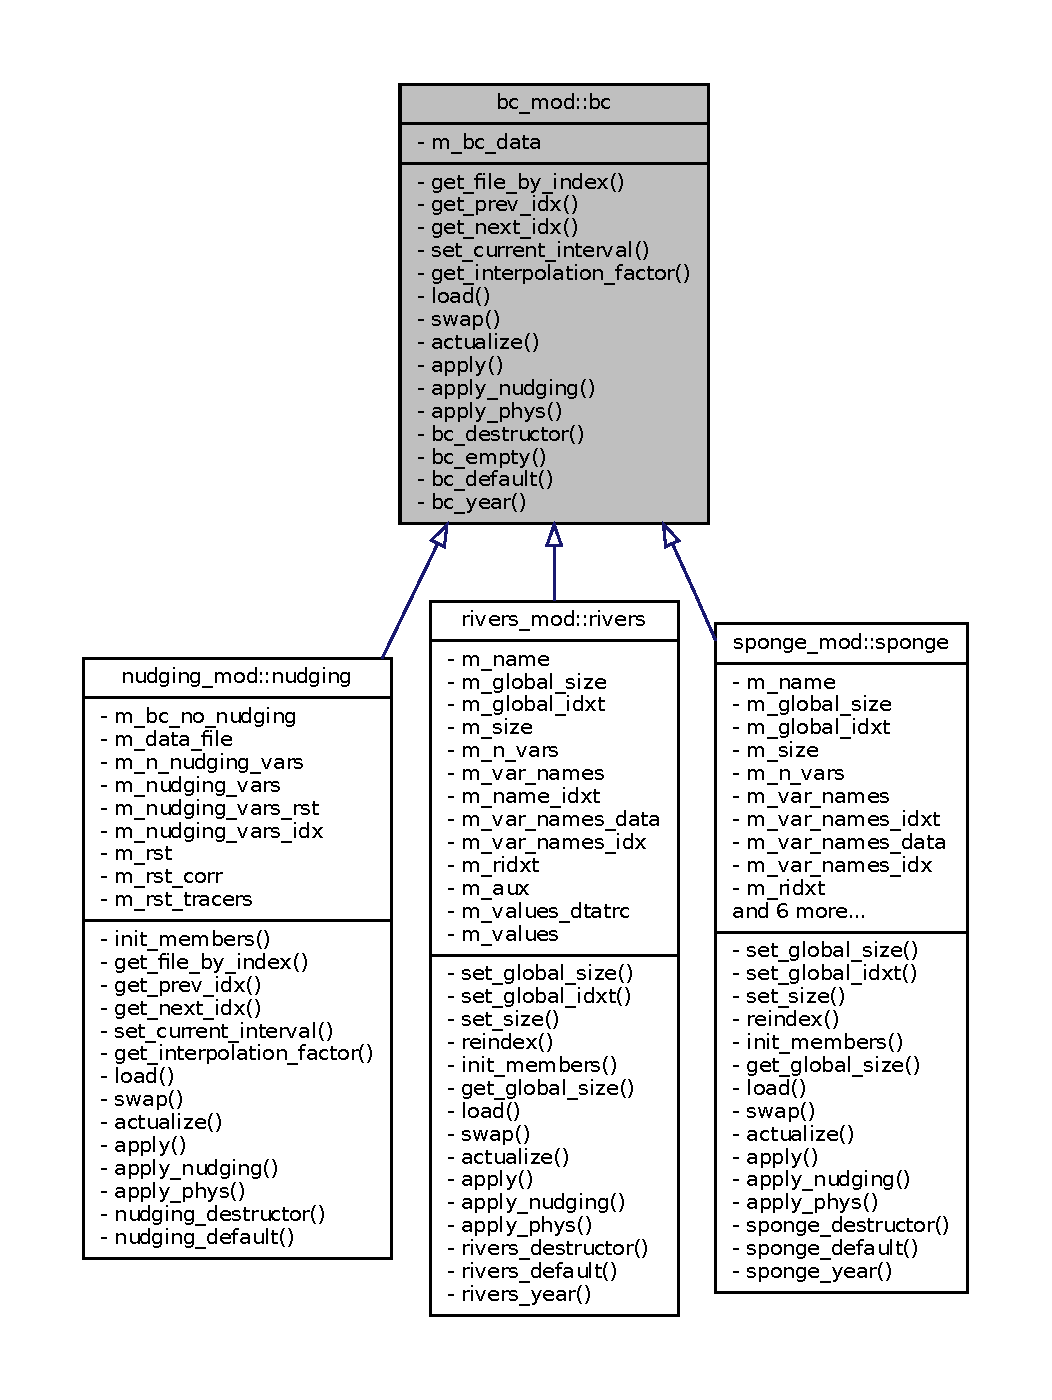
\includegraphics[width=350pt]{structbc__mod_1_1bc__inherit__graph}
\end{center}
\end{figure}
\subsubsection*{Private Member Functions}
\begin{DoxyCompactItemize}
\item 
procedure \mbox{\hyperlink{structbc__mod_1_1bc_aad031a20982832747243dc3e3fbfce20}{get\+\_\+file\+\_\+by\+\_\+index}}
\item 
procedure \mbox{\hyperlink{structbc__mod_1_1bc_aa04b9a462194855b7c9111fe67456f0d}{get\+\_\+prev\+\_\+idx}}
\item 
procedure \mbox{\hyperlink{structbc__mod_1_1bc_abf0c1a16ec610ce08ed379315afc7f55}{get\+\_\+next\+\_\+idx}}
\item 
procedure \mbox{\hyperlink{structbc__mod_1_1bc_adf9262a425534bd18d98809381034ca1}{set\+\_\+current\+\_\+interval}}
\item 
procedure \mbox{\hyperlink{structbc__mod_1_1bc_a1d7f33a1fd0c18e5ce50af4690c82846}{get\+\_\+interpolation\+\_\+factor}}
\item 
procedure \mbox{\hyperlink{structbc__mod_1_1bc_a1c4ee986270f18f4400c4554c06c5f7b}{load}}
\item 
procedure \mbox{\hyperlink{structbc__mod_1_1bc_a925ae5960dbfc854eab908c52c13f719}{swap}}
\item 
procedure \mbox{\hyperlink{structbc__mod_1_1bc_a15503494f181d4090774d948cecdce48}{actualize}}
\item 
procedure \mbox{\hyperlink{structbc__mod_1_1bc_a628eafc79842d1d1d62e043aedf49aa0}{apply}}
\item 
procedure \mbox{\hyperlink{structbc__mod_1_1bc_a42dc448ba9e50fbb6b1acf03b0d121f3}{apply\+\_\+nudging}}
\item 
procedure \mbox{\hyperlink{structbc__mod_1_1bc_ad0d03ece320569369a296ff3d4cf10d2}{apply\+\_\+phys}}
\item 
procedure \mbox{\hyperlink{structbc__mod_1_1bc_ad38c12a9f905c66965ffe633ead4edd2}{bc\+\_\+destructor}}
\item 
type(\mbox{\hyperlink{structbc__mod_1_1bc}{bc}}) function \mbox{\hyperlink{structbc__mod_1_1bc_a721ce450ae1ffdc8c9f0c8ef12f045d1}{bc\+\_\+empty}} ()
\item 
type(\mbox{\hyperlink{structbc__mod_1_1bc}{bc}}) function \mbox{\hyperlink{structbc__mod_1_1bc_a740cece69077685b30af7e619d448b33}{bc\+\_\+default}} (files\+\_\+namelist)
\item 
type(\mbox{\hyperlink{structbc__mod_1_1bc}{bc}}) function \mbox{\hyperlink{structbc__mod_1_1bc_ad1e474e0627921dd48884966e30f379d}{bc\+\_\+year}} (files\+\_\+namelist, start\+\_\+time\+\_\+string, end\+\_\+time\+\_\+string)
\end{DoxyCompactItemize}
\subsubsection*{Private Attributes}
\begin{DoxyCompactItemize}
\item 
type(\mbox{\hyperlink{structbc__data__mod_1_1bc__data}{bc\+\_\+data}}), pointer \mbox{\hyperlink{structbc__mod_1_1bc_a9ec09a6b6f5e1e75406505cb2851051a}{m\+\_\+bc\+\_\+data}} =$>$ null()
\end{DoxyCompactItemize}


\subsubsection{Member Function/\+Subroutine Documentation}
\mbox{\Hypertarget{structbc__mod_1_1bc_a15503494f181d4090774d948cecdce48}\label{structbc__mod_1_1bc_a15503494f181d4090774d948cecdce48}} 
\index{bc\+\_\+mod\+::bc@{bc\+\_\+mod\+::bc}!actualize@{actualize}}
\index{actualize@{actualize}!bc\+\_\+mod\+::bc@{bc\+\_\+mod\+::bc}}
\paragraph{\texorpdfstring{actualize()}{actualize()}}
{\footnotesize\ttfamily procedure bc\+\_\+mod\+::bc\+::actualize (\begin{DoxyParamCaption}{ }\end{DoxyParamCaption})\hspace{0.3cm}{\ttfamily [private]}}



Implemented in \mbox{\hyperlink{structsponge__mod_1_1sponge_a7d01836ef5f2e2ea4ee11a6c6231baed}{sponge\+\_\+mod\+::sponge}}, \mbox{\hyperlink{structrivers__mod_1_1rivers_a7c1b4c7a383553f4cacdae90725f3249}{rivers\+\_\+mod\+::rivers}}, and \mbox{\hyperlink{structnudging__mod_1_1nudging_ade178a579111036782c7b4570018f0d5}{nudging\+\_\+mod\+::nudging}}.

\mbox{\Hypertarget{structbc__mod_1_1bc_a628eafc79842d1d1d62e043aedf49aa0}\label{structbc__mod_1_1bc_a628eafc79842d1d1d62e043aedf49aa0}} 
\index{bc\+\_\+mod\+::bc@{bc\+\_\+mod\+::bc}!apply@{apply}}
\index{apply@{apply}!bc\+\_\+mod\+::bc@{bc\+\_\+mod\+::bc}}
\paragraph{\texorpdfstring{apply()}{apply()}}
{\footnotesize\ttfamily procedure bc\+\_\+mod\+::bc\+::apply (\begin{DoxyParamCaption}{ }\end{DoxyParamCaption})\hspace{0.3cm}{\ttfamily [private]}}



Implemented in \mbox{\hyperlink{structsponge__mod_1_1sponge_aca76f3cc282e1918ec76c8d6c34d4315}{sponge\+\_\+mod\+::sponge}}, \mbox{\hyperlink{structrivers__mod_1_1rivers_a97eb13e48a07c9020cb1b353d42a5466}{rivers\+\_\+mod\+::rivers}}, and \mbox{\hyperlink{structnudging__mod_1_1nudging_ad5101760abbec7a50024ecc3435eda49}{nudging\+\_\+mod\+::nudging}}.

\mbox{\Hypertarget{structbc__mod_1_1bc_a42dc448ba9e50fbb6b1acf03b0d121f3}\label{structbc__mod_1_1bc_a42dc448ba9e50fbb6b1acf03b0d121f3}} 
\index{bc\+\_\+mod\+::bc@{bc\+\_\+mod\+::bc}!apply\+\_\+nudging@{apply\+\_\+nudging}}
\index{apply\+\_\+nudging@{apply\+\_\+nudging}!bc\+\_\+mod\+::bc@{bc\+\_\+mod\+::bc}}
\paragraph{\texorpdfstring{apply\+\_\+nudging()}{apply\_nudging()}}
{\footnotesize\ttfamily procedure bc\+\_\+mod\+::bc\+::apply\+\_\+nudging (\begin{DoxyParamCaption}{ }\end{DoxyParamCaption})\hspace{0.3cm}{\ttfamily [private]}}



Implemented in \mbox{\hyperlink{structsponge__mod_1_1sponge_a8617d126acfe553a2d478258adaf029f}{sponge\+\_\+mod\+::sponge}}, \mbox{\hyperlink{structrivers__mod_1_1rivers_aaa8c35a085317190f69e097caba60cfb}{rivers\+\_\+mod\+::rivers}}, and \mbox{\hyperlink{structnudging__mod_1_1nudging_a232a6666abdc760493681d65cf8eb8e0}{nudging\+\_\+mod\+::nudging}}.

\mbox{\Hypertarget{structbc__mod_1_1bc_ad0d03ece320569369a296ff3d4cf10d2}\label{structbc__mod_1_1bc_ad0d03ece320569369a296ff3d4cf10d2}} 
\index{bc\+\_\+mod\+::bc@{bc\+\_\+mod\+::bc}!apply\+\_\+phys@{apply\+\_\+phys}}
\index{apply\+\_\+phys@{apply\+\_\+phys}!bc\+\_\+mod\+::bc@{bc\+\_\+mod\+::bc}}
\paragraph{\texorpdfstring{apply\+\_\+phys()}{apply\_phys()}}
{\footnotesize\ttfamily procedure bc\+\_\+mod\+::bc\+::apply\+\_\+phys (\begin{DoxyParamCaption}{ }\end{DoxyParamCaption})\hspace{0.3cm}{\ttfamily [private]}}



Implemented in \mbox{\hyperlink{structsponge__mod_1_1sponge_ab3f6fd55b37a4a4ba7fe9d0ac9f7b9ac}{sponge\+\_\+mod\+::sponge}}, \mbox{\hyperlink{structrivers__mod_1_1rivers_a4f6360b228319a4189289cafc2e3fd74}{rivers\+\_\+mod\+::rivers}}, and \mbox{\hyperlink{structnudging__mod_1_1nudging_a5e52b19bbb3e3481ebaa885040e92802}{nudging\+\_\+mod\+::nudging}}.

\mbox{\Hypertarget{structbc__mod_1_1bc_a740cece69077685b30af7e619d448b33}\label{structbc__mod_1_1bc_a740cece69077685b30af7e619d448b33}} 
\index{bc\+\_\+mod\+::bc@{bc\+\_\+mod\+::bc}!bc\+\_\+default@{bc\+\_\+default}}
\index{bc\+\_\+default@{bc\+\_\+default}!bc\+\_\+mod\+::bc@{bc\+\_\+mod\+::bc}}
\paragraph{\texorpdfstring{bc\+\_\+default()}{bc\_default()}}
{\footnotesize\ttfamily type(\mbox{\hyperlink{structbc__mod_1_1bc}{bc}}) function bc\+\_\+mod\+::bc\+::bc\+\_\+default (\begin{DoxyParamCaption}\item[{character(len=22), intent(in)}]{files\+\_\+namelist }\end{DoxyParamCaption})\hspace{0.3cm}{\ttfamily [private]}}

\mbox{\Hypertarget{structbc__mod_1_1bc_ad38c12a9f905c66965ffe633ead4edd2}\label{structbc__mod_1_1bc_ad38c12a9f905c66965ffe633ead4edd2}} 
\index{bc\+\_\+mod\+::bc@{bc\+\_\+mod\+::bc}!bc\+\_\+destructor@{bc\+\_\+destructor}}
\index{bc\+\_\+destructor@{bc\+\_\+destructor}!bc\+\_\+mod\+::bc@{bc\+\_\+mod\+::bc}}
\paragraph{\texorpdfstring{bc\+\_\+destructor()}{bc\_destructor()}}
{\footnotesize\ttfamily procedure bc\+\_\+mod\+::bc\+::bc\+\_\+destructor (\begin{DoxyParamCaption}{ }\end{DoxyParamCaption})\hspace{0.3cm}{\ttfamily [private]}}

\mbox{\Hypertarget{structbc__mod_1_1bc_a721ce450ae1ffdc8c9f0c8ef12f045d1}\label{structbc__mod_1_1bc_a721ce450ae1ffdc8c9f0c8ef12f045d1}} 
\index{bc\+\_\+mod\+::bc@{bc\+\_\+mod\+::bc}!bc\+\_\+empty@{bc\+\_\+empty}}
\index{bc\+\_\+empty@{bc\+\_\+empty}!bc\+\_\+mod\+::bc@{bc\+\_\+mod\+::bc}}
\paragraph{\texorpdfstring{bc\+\_\+empty()}{bc\_empty()}}
{\footnotesize\ttfamily type(\mbox{\hyperlink{structbc__mod_1_1bc}{bc}}) function bc\+\_\+mod\+::bc\+::bc\+\_\+empty (\begin{DoxyParamCaption}{ }\end{DoxyParamCaption})\hspace{0.3cm}{\ttfamily [private]}}

\mbox{\Hypertarget{structbc__mod_1_1bc_ad1e474e0627921dd48884966e30f379d}\label{structbc__mod_1_1bc_ad1e474e0627921dd48884966e30f379d}} 
\index{bc\+\_\+mod\+::bc@{bc\+\_\+mod\+::bc}!bc\+\_\+year@{bc\+\_\+year}}
\index{bc\+\_\+year@{bc\+\_\+year}!bc\+\_\+mod\+::bc@{bc\+\_\+mod\+::bc}}
\paragraph{\texorpdfstring{bc\+\_\+year()}{bc\_year()}}
{\footnotesize\ttfamily type(\mbox{\hyperlink{structbc__mod_1_1bc}{bc}}) function bc\+\_\+mod\+::bc\+::bc\+\_\+year (\begin{DoxyParamCaption}\item[{character(len=27), intent(in)}]{files\+\_\+namelist,  }\item[{character(len=17), intent(in)}]{start\+\_\+time\+\_\+string,  }\item[{character(len=17), intent(in)}]{end\+\_\+time\+\_\+string }\end{DoxyParamCaption})\hspace{0.3cm}{\ttfamily [private]}}

\mbox{\Hypertarget{structbc__mod_1_1bc_aad031a20982832747243dc3e3fbfce20}\label{structbc__mod_1_1bc_aad031a20982832747243dc3e3fbfce20}} 
\index{bc\+\_\+mod\+::bc@{bc\+\_\+mod\+::bc}!get\+\_\+file\+\_\+by\+\_\+index@{get\+\_\+file\+\_\+by\+\_\+index}}
\index{get\+\_\+file\+\_\+by\+\_\+index@{get\+\_\+file\+\_\+by\+\_\+index}!bc\+\_\+mod\+::bc@{bc\+\_\+mod\+::bc}}
\paragraph{\texorpdfstring{get\+\_\+file\+\_\+by\+\_\+index()}{get\_file\_by\_index()}}
{\footnotesize\ttfamily procedure bc\+\_\+mod\+::bc\+::get\+\_\+file\+\_\+by\+\_\+index (\begin{DoxyParamCaption}{ }\end{DoxyParamCaption})\hspace{0.3cm}{\ttfamily [private]}}



Implemented in \mbox{\hyperlink{structnudging__mod_1_1nudging_a76b1b1b5a273bab2e43348de8c7721c6}{nudging\+\_\+mod\+::nudging}}.

\mbox{\Hypertarget{structbc__mod_1_1bc_a1d7f33a1fd0c18e5ce50af4690c82846}\label{structbc__mod_1_1bc_a1d7f33a1fd0c18e5ce50af4690c82846}} 
\index{bc\+\_\+mod\+::bc@{bc\+\_\+mod\+::bc}!get\+\_\+interpolation\+\_\+factor@{get\+\_\+interpolation\+\_\+factor}}
\index{get\+\_\+interpolation\+\_\+factor@{get\+\_\+interpolation\+\_\+factor}!bc\+\_\+mod\+::bc@{bc\+\_\+mod\+::bc}}
\paragraph{\texorpdfstring{get\+\_\+interpolation\+\_\+factor()}{get\_interpolation\_factor()}}
{\footnotesize\ttfamily procedure bc\+\_\+mod\+::bc\+::get\+\_\+interpolation\+\_\+factor (\begin{DoxyParamCaption}{ }\end{DoxyParamCaption})\hspace{0.3cm}{\ttfamily [private]}}



Implemented in \mbox{\hyperlink{structnudging__mod_1_1nudging_a55ee89e52a1b3b98d4ff84802f888dd4}{nudging\+\_\+mod\+::nudging}}.

\mbox{\Hypertarget{structbc__mod_1_1bc_abf0c1a16ec610ce08ed379315afc7f55}\label{structbc__mod_1_1bc_abf0c1a16ec610ce08ed379315afc7f55}} 
\index{bc\+\_\+mod\+::bc@{bc\+\_\+mod\+::bc}!get\+\_\+next\+\_\+idx@{get\+\_\+next\+\_\+idx}}
\index{get\+\_\+next\+\_\+idx@{get\+\_\+next\+\_\+idx}!bc\+\_\+mod\+::bc@{bc\+\_\+mod\+::bc}}
\paragraph{\texorpdfstring{get\+\_\+next\+\_\+idx()}{get\_next\_idx()}}
{\footnotesize\ttfamily procedure bc\+\_\+mod\+::bc\+::get\+\_\+next\+\_\+idx (\begin{DoxyParamCaption}{ }\end{DoxyParamCaption})\hspace{0.3cm}{\ttfamily [private]}}



Implemented in \mbox{\hyperlink{structnudging__mod_1_1nudging_afd2889fe6e9aa9560ebb2358efba4dec}{nudging\+\_\+mod\+::nudging}}.

\mbox{\Hypertarget{structbc__mod_1_1bc_aa04b9a462194855b7c9111fe67456f0d}\label{structbc__mod_1_1bc_aa04b9a462194855b7c9111fe67456f0d}} 
\index{bc\+\_\+mod\+::bc@{bc\+\_\+mod\+::bc}!get\+\_\+prev\+\_\+idx@{get\+\_\+prev\+\_\+idx}}
\index{get\+\_\+prev\+\_\+idx@{get\+\_\+prev\+\_\+idx}!bc\+\_\+mod\+::bc@{bc\+\_\+mod\+::bc}}
\paragraph{\texorpdfstring{get\+\_\+prev\+\_\+idx()}{get\_prev\_idx()}}
{\footnotesize\ttfamily procedure bc\+\_\+mod\+::bc\+::get\+\_\+prev\+\_\+idx (\begin{DoxyParamCaption}{ }\end{DoxyParamCaption})\hspace{0.3cm}{\ttfamily [private]}}



Implemented in \mbox{\hyperlink{structnudging__mod_1_1nudging_ad1d7271784597d454bc97108232613cd}{nudging\+\_\+mod\+::nudging}}.

\mbox{\Hypertarget{structbc__mod_1_1bc_a1c4ee986270f18f4400c4554c06c5f7b}\label{structbc__mod_1_1bc_a1c4ee986270f18f4400c4554c06c5f7b}} 
\index{bc\+\_\+mod\+::bc@{bc\+\_\+mod\+::bc}!load@{load}}
\index{load@{load}!bc\+\_\+mod\+::bc@{bc\+\_\+mod\+::bc}}
\paragraph{\texorpdfstring{load()}{load()}}
{\footnotesize\ttfamily procedure bc\+\_\+mod\+::bc\+::load (\begin{DoxyParamCaption}{ }\end{DoxyParamCaption})\hspace{0.3cm}{\ttfamily [private]}}



Implemented in \mbox{\hyperlink{structsponge__mod_1_1sponge_a0383aabeecf15b7c47bc43c9b4746c60}{sponge\+\_\+mod\+::sponge}}, \mbox{\hyperlink{structrivers__mod_1_1rivers_a4eac45372772ea12c7f18505a4de53ee}{rivers\+\_\+mod\+::rivers}}, and \mbox{\hyperlink{structnudging__mod_1_1nudging_ad0fe3f6011636572c0641ef4b01bba33}{nudging\+\_\+mod\+::nudging}}.

\mbox{\Hypertarget{structbc__mod_1_1bc_adf9262a425534bd18d98809381034ca1}\label{structbc__mod_1_1bc_adf9262a425534bd18d98809381034ca1}} 
\index{bc\+\_\+mod\+::bc@{bc\+\_\+mod\+::bc}!set\+\_\+current\+\_\+interval@{set\+\_\+current\+\_\+interval}}
\index{set\+\_\+current\+\_\+interval@{set\+\_\+current\+\_\+interval}!bc\+\_\+mod\+::bc@{bc\+\_\+mod\+::bc}}
\paragraph{\texorpdfstring{set\+\_\+current\+\_\+interval()}{set\_current\_interval()}}
{\footnotesize\ttfamily procedure bc\+\_\+mod\+::bc\+::set\+\_\+current\+\_\+interval (\begin{DoxyParamCaption}{ }\end{DoxyParamCaption})\hspace{0.3cm}{\ttfamily [private]}}



Implemented in \mbox{\hyperlink{structnudging__mod_1_1nudging_ab17fe87aa8dc77bd4bf0cba14d68969a}{nudging\+\_\+mod\+::nudging}}.

\mbox{\Hypertarget{structbc__mod_1_1bc_a925ae5960dbfc854eab908c52c13f719}\label{structbc__mod_1_1bc_a925ae5960dbfc854eab908c52c13f719}} 
\index{bc\+\_\+mod\+::bc@{bc\+\_\+mod\+::bc}!swap@{swap}}
\index{swap@{swap}!bc\+\_\+mod\+::bc@{bc\+\_\+mod\+::bc}}
\paragraph{\texorpdfstring{swap()}{swap()}}
{\footnotesize\ttfamily procedure bc\+\_\+mod\+::bc\+::swap (\begin{DoxyParamCaption}{ }\end{DoxyParamCaption})\hspace{0.3cm}{\ttfamily [private]}}



Implemented in \mbox{\hyperlink{structsponge__mod_1_1sponge_abe0102a0a72e189b8871724a21680c43}{sponge\+\_\+mod\+::sponge}}, \mbox{\hyperlink{structrivers__mod_1_1rivers_a7bcfc95d699f097aed2975941cabe059}{rivers\+\_\+mod\+::rivers}}, and \mbox{\hyperlink{structnudging__mod_1_1nudging_a9015b684c729f54ba0fe1abc15b28a49}{nudging\+\_\+mod\+::nudging}}.



\subsubsection{Member Data Documentation}
\mbox{\Hypertarget{structbc__mod_1_1bc_a9ec09a6b6f5e1e75406505cb2851051a}\label{structbc__mod_1_1bc_a9ec09a6b6f5e1e75406505cb2851051a}} 
\index{bc\+\_\+mod\+::bc@{bc\+\_\+mod\+::bc}!m\+\_\+bc\+\_\+data@{m\+\_\+bc\+\_\+data}}
\index{m\+\_\+bc\+\_\+data@{m\+\_\+bc\+\_\+data}!bc\+\_\+mod\+::bc@{bc\+\_\+mod\+::bc}}
\paragraph{\texorpdfstring{m\+\_\+bc\+\_\+data}{m\_bc\_data}}
{\footnotesize\ttfamily type(\mbox{\hyperlink{structbc__data__mod_1_1bc__data}{bc\+\_\+data}}), pointer bc\+\_\+mod\+::bc\+::m\+\_\+bc\+\_\+data =$>$ null()\hspace{0.3cm}{\ttfamily [private]}}


\hypertarget{structbc__data__mod_1_1bc__data}{}\subsection{bc\+\_\+data\+\_\+mod\+:\+:bc\+\_\+data Interface Reference}
\label{structbc__data__mod_1_1bc__data}\index{bc\+\_\+data\+\_\+mod\+::bc\+\_\+data@{bc\+\_\+data\+\_\+mod\+::bc\+\_\+data}}
\subsubsection*{Private Member Functions}
\begin{DoxyCompactItemize}
\item 
procedure \mbox{\hyperlink{structbc__data__mod_1_1bc__data_a41f21b3b50a142b75b72783201138764}{get\+\_\+file\+\_\+by\+\_\+index}}
\item 
procedure \mbox{\hyperlink{structbc__data__mod_1_1bc__data_a895282cf8decbb94b2fdd38a1d521a9a}{get\+\_\+prev\+\_\+idx}}
\item 
procedure \mbox{\hyperlink{structbc__data__mod_1_1bc__data_a2ce00fac38a7480080678d5e1aa10a76}{get\+\_\+next\+\_\+idx}}
\item 
procedure \mbox{\hyperlink{structbc__data__mod_1_1bc__data_a7cffb1d5013154bd042c821ad54c32fa}{set\+\_\+current\+\_\+interval}}
\item 
procedure \mbox{\hyperlink{structbc__data__mod_1_1bc__data_a349ac8feea73d8b81f701430b13da35e}{get\+\_\+interpolation\+\_\+factor}}
\item 
procedure \mbox{\hyperlink{structbc__data__mod_1_1bc__data_ab06868f3da529de5d889c8bf857f8a4d}{new\+\_\+interval}}
\item 
procedure \mbox{\hyperlink{structbc__data__mod_1_1bc__data_a459fdc4d5aaf79feb770e526911463e6}{bc\+\_\+data\+\_\+destructor}}
\item 
type(\mbox{\hyperlink{structbc__data__mod_1_1bc__data}{bc\+\_\+data}}) function \mbox{\hyperlink{structbc__data__mod_1_1bc__data_a6b0b86345c37a378d6fa2fdcfc6a823a}{bc\+\_\+data\+\_\+empty}} ()
\item 
type(\mbox{\hyperlink{structbc__data__mod_1_1bc__data}{bc\+\_\+data}}) function \mbox{\hyperlink{structbc__data__mod_1_1bc__data_aa4e512b1f44734058e9475f8c57636c7}{bc\+\_\+data\+\_\+default}} (files\+\_\+namelist)
\item 
type(\mbox{\hyperlink{structbc__data__mod_1_1bc__data}{bc\+\_\+data}}) function \mbox{\hyperlink{structbc__data__mod_1_1bc__data_a5a6932f22b635060341c6aaf512eb656}{bc\+\_\+data\+\_\+year}} (files\+\_\+namelist, start\+\_\+time\+\_\+string, end\+\_\+time\+\_\+string)
\end{DoxyCompactItemize}
\subsubsection*{Private Attributes}
\begin{DoxyCompactItemize}
\item 
integer \mbox{\hyperlink{structbc__data__mod_1_1bc__data_a49a8569566c05d9bbab1d8592252d126}{m\+\_\+n\+\_\+files}}
\item 
character(len=24), dimension(\+:), allocatable \mbox{\hyperlink{structbc__data__mod_1_1bc__data_a5785afc144fb332bc2192e16ca6cfc4c}{m\+\_\+files}}
\item 
character(len=17), dimension(\+:), allocatable \mbox{\hyperlink{structbc__data__mod_1_1bc__data_a4bc7f15cecef9103e9cffdd2dc207935}{m\+\_\+time\+\_\+strings}}
\item 
integer \mbox{\hyperlink{structbc__data__mod_1_1bc__data_ac59b5fae46e0c7bf5b0f56aca59bb273}{m\+\_\+n\+\_\+times}}
\item 
double precision, dimension(\+:), allocatable \mbox{\hyperlink{structbc__data__mod_1_1bc__data_a92c42d3e066a22a473ab21707edf3fda}{m\+\_\+times}}
\item 
integer \mbox{\hyperlink{structbc__data__mod_1_1bc__data_a9483d31271a4d20b053aa437eee51b2b}{m\+\_\+prev\+\_\+idx}}
\item 
integer \mbox{\hyperlink{structbc__data__mod_1_1bc__data_adc45e6826431d7e49919491b7683c3fd}{m\+\_\+next\+\_\+idx}}
\item 
logical \mbox{\hyperlink{structbc__data__mod_1_1bc__data_a8d540dbf0910bb3307c2cd5573762306}{m\+\_\+new\+\_\+interval}}
\end{DoxyCompactItemize}


\subsubsection{Member Function/\+Subroutine Documentation}
\mbox{\Hypertarget{structbc__data__mod_1_1bc__data_aa4e512b1f44734058e9475f8c57636c7}\label{structbc__data__mod_1_1bc__data_aa4e512b1f44734058e9475f8c57636c7}} 
\index{bc\+\_\+data\+\_\+mod\+::bc\+\_\+data@{bc\+\_\+data\+\_\+mod\+::bc\+\_\+data}!bc\+\_\+data\+\_\+default@{bc\+\_\+data\+\_\+default}}
\index{bc\+\_\+data\+\_\+default@{bc\+\_\+data\+\_\+default}!bc\+\_\+data\+\_\+mod\+::bc\+\_\+data@{bc\+\_\+data\+\_\+mod\+::bc\+\_\+data}}
\paragraph{\texorpdfstring{bc\+\_\+data\+\_\+default()}{bc\_data\_default()}}
{\footnotesize\ttfamily type(\mbox{\hyperlink{structbc__data__mod_1_1bc__data}{bc\+\_\+data}}) function bc\+\_\+data\+\_\+mod\+::bc\+\_\+data\+::bc\+\_\+data\+\_\+default (\begin{DoxyParamCaption}\item[{character(len=22), intent(in)}]{files\+\_\+namelist }\end{DoxyParamCaption})\hspace{0.3cm}{\ttfamily [private]}}

\mbox{\Hypertarget{structbc__data__mod_1_1bc__data_a459fdc4d5aaf79feb770e526911463e6}\label{structbc__data__mod_1_1bc__data_a459fdc4d5aaf79feb770e526911463e6}} 
\index{bc\+\_\+data\+\_\+mod\+::bc\+\_\+data@{bc\+\_\+data\+\_\+mod\+::bc\+\_\+data}!bc\+\_\+data\+\_\+destructor@{bc\+\_\+data\+\_\+destructor}}
\index{bc\+\_\+data\+\_\+destructor@{bc\+\_\+data\+\_\+destructor}!bc\+\_\+data\+\_\+mod\+::bc\+\_\+data@{bc\+\_\+data\+\_\+mod\+::bc\+\_\+data}}
\paragraph{\texorpdfstring{bc\+\_\+data\+\_\+destructor()}{bc\_data\_destructor()}}
{\footnotesize\ttfamily procedure bc\+\_\+data\+\_\+mod\+::bc\+\_\+data\+::bc\+\_\+data\+\_\+destructor (\begin{DoxyParamCaption}{ }\end{DoxyParamCaption})\hspace{0.3cm}{\ttfamily [private]}}

\mbox{\Hypertarget{structbc__data__mod_1_1bc__data_a6b0b86345c37a378d6fa2fdcfc6a823a}\label{structbc__data__mod_1_1bc__data_a6b0b86345c37a378d6fa2fdcfc6a823a}} 
\index{bc\+\_\+data\+\_\+mod\+::bc\+\_\+data@{bc\+\_\+data\+\_\+mod\+::bc\+\_\+data}!bc\+\_\+data\+\_\+empty@{bc\+\_\+data\+\_\+empty}}
\index{bc\+\_\+data\+\_\+empty@{bc\+\_\+data\+\_\+empty}!bc\+\_\+data\+\_\+mod\+::bc\+\_\+data@{bc\+\_\+data\+\_\+mod\+::bc\+\_\+data}}
\paragraph{\texorpdfstring{bc\+\_\+data\+\_\+empty()}{bc\_data\_empty()}}
{\footnotesize\ttfamily type(\mbox{\hyperlink{structbc__data__mod_1_1bc__data}{bc\+\_\+data}}) function bc\+\_\+data\+\_\+mod\+::bc\+\_\+data\+::bc\+\_\+data\+\_\+empty (\begin{DoxyParamCaption}{ }\end{DoxyParamCaption})\hspace{0.3cm}{\ttfamily [private]}}

\mbox{\Hypertarget{structbc__data__mod_1_1bc__data_a5a6932f22b635060341c6aaf512eb656}\label{structbc__data__mod_1_1bc__data_a5a6932f22b635060341c6aaf512eb656}} 
\index{bc\+\_\+data\+\_\+mod\+::bc\+\_\+data@{bc\+\_\+data\+\_\+mod\+::bc\+\_\+data}!bc\+\_\+data\+\_\+year@{bc\+\_\+data\+\_\+year}}
\index{bc\+\_\+data\+\_\+year@{bc\+\_\+data\+\_\+year}!bc\+\_\+data\+\_\+mod\+::bc\+\_\+data@{bc\+\_\+data\+\_\+mod\+::bc\+\_\+data}}
\paragraph{\texorpdfstring{bc\+\_\+data\+\_\+year()}{bc\_data\_year()}}
{\footnotesize\ttfamily type(\mbox{\hyperlink{structbc__data__mod_1_1bc__data}{bc\+\_\+data}}) function bc\+\_\+data\+\_\+mod\+::bc\+\_\+data\+::bc\+\_\+data\+\_\+year (\begin{DoxyParamCaption}\item[{character(len=27), intent(in)}]{files\+\_\+namelist,  }\item[{character(len=17), intent(in)}]{start\+\_\+time\+\_\+string,  }\item[{character(len=17), intent(in)}]{end\+\_\+time\+\_\+string }\end{DoxyParamCaption})\hspace{0.3cm}{\ttfamily [private]}}

\mbox{\Hypertarget{structbc__data__mod_1_1bc__data_a41f21b3b50a142b75b72783201138764}\label{structbc__data__mod_1_1bc__data_a41f21b3b50a142b75b72783201138764}} 
\index{bc\+\_\+data\+\_\+mod\+::bc\+\_\+data@{bc\+\_\+data\+\_\+mod\+::bc\+\_\+data}!get\+\_\+file\+\_\+by\+\_\+index@{get\+\_\+file\+\_\+by\+\_\+index}}
\index{get\+\_\+file\+\_\+by\+\_\+index@{get\+\_\+file\+\_\+by\+\_\+index}!bc\+\_\+data\+\_\+mod\+::bc\+\_\+data@{bc\+\_\+data\+\_\+mod\+::bc\+\_\+data}}
\paragraph{\texorpdfstring{get\+\_\+file\+\_\+by\+\_\+index()}{get\_file\_by\_index()}}
{\footnotesize\ttfamily procedure bc\+\_\+data\+\_\+mod\+::bc\+\_\+data\+::get\+\_\+file\+\_\+by\+\_\+index (\begin{DoxyParamCaption}{ }\end{DoxyParamCaption})\hspace{0.3cm}{\ttfamily [private]}}

\mbox{\Hypertarget{structbc__data__mod_1_1bc__data_a349ac8feea73d8b81f701430b13da35e}\label{structbc__data__mod_1_1bc__data_a349ac8feea73d8b81f701430b13da35e}} 
\index{bc\+\_\+data\+\_\+mod\+::bc\+\_\+data@{bc\+\_\+data\+\_\+mod\+::bc\+\_\+data}!get\+\_\+interpolation\+\_\+factor@{get\+\_\+interpolation\+\_\+factor}}
\index{get\+\_\+interpolation\+\_\+factor@{get\+\_\+interpolation\+\_\+factor}!bc\+\_\+data\+\_\+mod\+::bc\+\_\+data@{bc\+\_\+data\+\_\+mod\+::bc\+\_\+data}}
\paragraph{\texorpdfstring{get\+\_\+interpolation\+\_\+factor()}{get\_interpolation\_factor()}}
{\footnotesize\ttfamily procedure bc\+\_\+data\+\_\+mod\+::bc\+\_\+data\+::get\+\_\+interpolation\+\_\+factor (\begin{DoxyParamCaption}{ }\end{DoxyParamCaption})\hspace{0.3cm}{\ttfamily [private]}}

\mbox{\Hypertarget{structbc__data__mod_1_1bc__data_a2ce00fac38a7480080678d5e1aa10a76}\label{structbc__data__mod_1_1bc__data_a2ce00fac38a7480080678d5e1aa10a76}} 
\index{bc\+\_\+data\+\_\+mod\+::bc\+\_\+data@{bc\+\_\+data\+\_\+mod\+::bc\+\_\+data}!get\+\_\+next\+\_\+idx@{get\+\_\+next\+\_\+idx}}
\index{get\+\_\+next\+\_\+idx@{get\+\_\+next\+\_\+idx}!bc\+\_\+data\+\_\+mod\+::bc\+\_\+data@{bc\+\_\+data\+\_\+mod\+::bc\+\_\+data}}
\paragraph{\texorpdfstring{get\+\_\+next\+\_\+idx()}{get\_next\_idx()}}
{\footnotesize\ttfamily procedure bc\+\_\+data\+\_\+mod\+::bc\+\_\+data\+::get\+\_\+next\+\_\+idx (\begin{DoxyParamCaption}{ }\end{DoxyParamCaption})\hspace{0.3cm}{\ttfamily [private]}}

\mbox{\Hypertarget{structbc__data__mod_1_1bc__data_a895282cf8decbb94b2fdd38a1d521a9a}\label{structbc__data__mod_1_1bc__data_a895282cf8decbb94b2fdd38a1d521a9a}} 
\index{bc\+\_\+data\+\_\+mod\+::bc\+\_\+data@{bc\+\_\+data\+\_\+mod\+::bc\+\_\+data}!get\+\_\+prev\+\_\+idx@{get\+\_\+prev\+\_\+idx}}
\index{get\+\_\+prev\+\_\+idx@{get\+\_\+prev\+\_\+idx}!bc\+\_\+data\+\_\+mod\+::bc\+\_\+data@{bc\+\_\+data\+\_\+mod\+::bc\+\_\+data}}
\paragraph{\texorpdfstring{get\+\_\+prev\+\_\+idx()}{get\_prev\_idx()}}
{\footnotesize\ttfamily procedure bc\+\_\+data\+\_\+mod\+::bc\+\_\+data\+::get\+\_\+prev\+\_\+idx (\begin{DoxyParamCaption}{ }\end{DoxyParamCaption})\hspace{0.3cm}{\ttfamily [private]}}

\mbox{\Hypertarget{structbc__data__mod_1_1bc__data_ab06868f3da529de5d889c8bf857f8a4d}\label{structbc__data__mod_1_1bc__data_ab06868f3da529de5d889c8bf857f8a4d}} 
\index{bc\+\_\+data\+\_\+mod\+::bc\+\_\+data@{bc\+\_\+data\+\_\+mod\+::bc\+\_\+data}!new\+\_\+interval@{new\+\_\+interval}}
\index{new\+\_\+interval@{new\+\_\+interval}!bc\+\_\+data\+\_\+mod\+::bc\+\_\+data@{bc\+\_\+data\+\_\+mod\+::bc\+\_\+data}}
\paragraph{\texorpdfstring{new\+\_\+interval()}{new\_interval()}}
{\footnotesize\ttfamily procedure bc\+\_\+data\+\_\+mod\+::bc\+\_\+data\+::new\+\_\+interval (\begin{DoxyParamCaption}{ }\end{DoxyParamCaption})\hspace{0.3cm}{\ttfamily [private]}}

\mbox{\Hypertarget{structbc__data__mod_1_1bc__data_a7cffb1d5013154bd042c821ad54c32fa}\label{structbc__data__mod_1_1bc__data_a7cffb1d5013154bd042c821ad54c32fa}} 
\index{bc\+\_\+data\+\_\+mod\+::bc\+\_\+data@{bc\+\_\+data\+\_\+mod\+::bc\+\_\+data}!set\+\_\+current\+\_\+interval@{set\+\_\+current\+\_\+interval}}
\index{set\+\_\+current\+\_\+interval@{set\+\_\+current\+\_\+interval}!bc\+\_\+data\+\_\+mod\+::bc\+\_\+data@{bc\+\_\+data\+\_\+mod\+::bc\+\_\+data}}
\paragraph{\texorpdfstring{set\+\_\+current\+\_\+interval()}{set\_current\_interval()}}
{\footnotesize\ttfamily procedure bc\+\_\+data\+\_\+mod\+::bc\+\_\+data\+::set\+\_\+current\+\_\+interval (\begin{DoxyParamCaption}{ }\end{DoxyParamCaption})\hspace{0.3cm}{\ttfamily [private]}}



\subsubsection{Member Data Documentation}
\mbox{\Hypertarget{structbc__data__mod_1_1bc__data_a5785afc144fb332bc2192e16ca6cfc4c}\label{structbc__data__mod_1_1bc__data_a5785afc144fb332bc2192e16ca6cfc4c}} 
\index{bc\+\_\+data\+\_\+mod\+::bc\+\_\+data@{bc\+\_\+data\+\_\+mod\+::bc\+\_\+data}!m\+\_\+files@{m\+\_\+files}}
\index{m\+\_\+files@{m\+\_\+files}!bc\+\_\+data\+\_\+mod\+::bc\+\_\+data@{bc\+\_\+data\+\_\+mod\+::bc\+\_\+data}}
\paragraph{\texorpdfstring{m\+\_\+files}{m\_files}}
{\footnotesize\ttfamily character(len=24), dimension(\+:), allocatable bc\+\_\+data\+\_\+mod\+::bc\+\_\+data\+::m\+\_\+files\hspace{0.3cm}{\ttfamily [private]}}

\mbox{\Hypertarget{structbc__data__mod_1_1bc__data_a49a8569566c05d9bbab1d8592252d126}\label{structbc__data__mod_1_1bc__data_a49a8569566c05d9bbab1d8592252d126}} 
\index{bc\+\_\+data\+\_\+mod\+::bc\+\_\+data@{bc\+\_\+data\+\_\+mod\+::bc\+\_\+data}!m\+\_\+n\+\_\+files@{m\+\_\+n\+\_\+files}}
\index{m\+\_\+n\+\_\+files@{m\+\_\+n\+\_\+files}!bc\+\_\+data\+\_\+mod\+::bc\+\_\+data@{bc\+\_\+data\+\_\+mod\+::bc\+\_\+data}}
\paragraph{\texorpdfstring{m\+\_\+n\+\_\+files}{m\_n\_files}}
{\footnotesize\ttfamily integer bc\+\_\+data\+\_\+mod\+::bc\+\_\+data\+::m\+\_\+n\+\_\+files\hspace{0.3cm}{\ttfamily [private]}}

\mbox{\Hypertarget{structbc__data__mod_1_1bc__data_ac59b5fae46e0c7bf5b0f56aca59bb273}\label{structbc__data__mod_1_1bc__data_ac59b5fae46e0c7bf5b0f56aca59bb273}} 
\index{bc\+\_\+data\+\_\+mod\+::bc\+\_\+data@{bc\+\_\+data\+\_\+mod\+::bc\+\_\+data}!m\+\_\+n\+\_\+times@{m\+\_\+n\+\_\+times}}
\index{m\+\_\+n\+\_\+times@{m\+\_\+n\+\_\+times}!bc\+\_\+data\+\_\+mod\+::bc\+\_\+data@{bc\+\_\+data\+\_\+mod\+::bc\+\_\+data}}
\paragraph{\texorpdfstring{m\+\_\+n\+\_\+times}{m\_n\_times}}
{\footnotesize\ttfamily integer bc\+\_\+data\+\_\+mod\+::bc\+\_\+data\+::m\+\_\+n\+\_\+times\hspace{0.3cm}{\ttfamily [private]}}

\mbox{\Hypertarget{structbc__data__mod_1_1bc__data_a8d540dbf0910bb3307c2cd5573762306}\label{structbc__data__mod_1_1bc__data_a8d540dbf0910bb3307c2cd5573762306}} 
\index{bc\+\_\+data\+\_\+mod\+::bc\+\_\+data@{bc\+\_\+data\+\_\+mod\+::bc\+\_\+data}!m\+\_\+new\+\_\+interval@{m\+\_\+new\+\_\+interval}}
\index{m\+\_\+new\+\_\+interval@{m\+\_\+new\+\_\+interval}!bc\+\_\+data\+\_\+mod\+::bc\+\_\+data@{bc\+\_\+data\+\_\+mod\+::bc\+\_\+data}}
\paragraph{\texorpdfstring{m\+\_\+new\+\_\+interval}{m\_new\_interval}}
{\footnotesize\ttfamily logical bc\+\_\+data\+\_\+mod\+::bc\+\_\+data\+::m\+\_\+new\+\_\+interval\hspace{0.3cm}{\ttfamily [private]}}

\mbox{\Hypertarget{structbc__data__mod_1_1bc__data_adc45e6826431d7e49919491b7683c3fd}\label{structbc__data__mod_1_1bc__data_adc45e6826431d7e49919491b7683c3fd}} 
\index{bc\+\_\+data\+\_\+mod\+::bc\+\_\+data@{bc\+\_\+data\+\_\+mod\+::bc\+\_\+data}!m\+\_\+next\+\_\+idx@{m\+\_\+next\+\_\+idx}}
\index{m\+\_\+next\+\_\+idx@{m\+\_\+next\+\_\+idx}!bc\+\_\+data\+\_\+mod\+::bc\+\_\+data@{bc\+\_\+data\+\_\+mod\+::bc\+\_\+data}}
\paragraph{\texorpdfstring{m\+\_\+next\+\_\+idx}{m\_next\_idx}}
{\footnotesize\ttfamily integer bc\+\_\+data\+\_\+mod\+::bc\+\_\+data\+::m\+\_\+next\+\_\+idx\hspace{0.3cm}{\ttfamily [private]}}

\mbox{\Hypertarget{structbc__data__mod_1_1bc__data_a9483d31271a4d20b053aa437eee51b2b}\label{structbc__data__mod_1_1bc__data_a9483d31271a4d20b053aa437eee51b2b}} 
\index{bc\+\_\+data\+\_\+mod\+::bc\+\_\+data@{bc\+\_\+data\+\_\+mod\+::bc\+\_\+data}!m\+\_\+prev\+\_\+idx@{m\+\_\+prev\+\_\+idx}}
\index{m\+\_\+prev\+\_\+idx@{m\+\_\+prev\+\_\+idx}!bc\+\_\+data\+\_\+mod\+::bc\+\_\+data@{bc\+\_\+data\+\_\+mod\+::bc\+\_\+data}}
\paragraph{\texorpdfstring{m\+\_\+prev\+\_\+idx}{m\_prev\_idx}}
{\footnotesize\ttfamily integer bc\+\_\+data\+\_\+mod\+::bc\+\_\+data\+::m\+\_\+prev\+\_\+idx\hspace{0.3cm}{\ttfamily [private]}}

\mbox{\Hypertarget{structbc__data__mod_1_1bc__data_a4bc7f15cecef9103e9cffdd2dc207935}\label{structbc__data__mod_1_1bc__data_a4bc7f15cecef9103e9cffdd2dc207935}} 
\index{bc\+\_\+data\+\_\+mod\+::bc\+\_\+data@{bc\+\_\+data\+\_\+mod\+::bc\+\_\+data}!m\+\_\+time\+\_\+strings@{m\+\_\+time\+\_\+strings}}
\index{m\+\_\+time\+\_\+strings@{m\+\_\+time\+\_\+strings}!bc\+\_\+data\+\_\+mod\+::bc\+\_\+data@{bc\+\_\+data\+\_\+mod\+::bc\+\_\+data}}
\paragraph{\texorpdfstring{m\+\_\+time\+\_\+strings}{m\_time\_strings}}
{\footnotesize\ttfamily character(len=17), dimension(\+:), allocatable bc\+\_\+data\+\_\+mod\+::bc\+\_\+data\+::m\+\_\+time\+\_\+strings\hspace{0.3cm}{\ttfamily [private]}}

\mbox{\Hypertarget{structbc__data__mod_1_1bc__data_a92c42d3e066a22a473ab21707edf3fda}\label{structbc__data__mod_1_1bc__data_a92c42d3e066a22a473ab21707edf3fda}} 
\index{bc\+\_\+data\+\_\+mod\+::bc\+\_\+data@{bc\+\_\+data\+\_\+mod\+::bc\+\_\+data}!m\+\_\+times@{m\+\_\+times}}
\index{m\+\_\+times@{m\+\_\+times}!bc\+\_\+data\+\_\+mod\+::bc\+\_\+data@{bc\+\_\+data\+\_\+mod\+::bc\+\_\+data}}
\paragraph{\texorpdfstring{m\+\_\+times}{m\_times}}
{\footnotesize\ttfamily double precision, dimension(\+:), allocatable bc\+\_\+data\+\_\+mod\+::bc\+\_\+data\+::m\+\_\+times\hspace{0.3cm}{\ttfamily [private]}}


\hypertarget{structnudging__mod_1_1nudging}{}\subsection{nudging\+\_\+mod\+:\+:nudging Interface Reference}
\label{structnudging__mod_1_1nudging}\index{nudging\+\_\+mod\+::nudging@{nudging\+\_\+mod\+::nudging}}


Inheritance diagram for nudging\+\_\+mod\+:\+:nudging\+:
\nopagebreak
\begin{figure}[H]
\begin{center}
\leavevmode
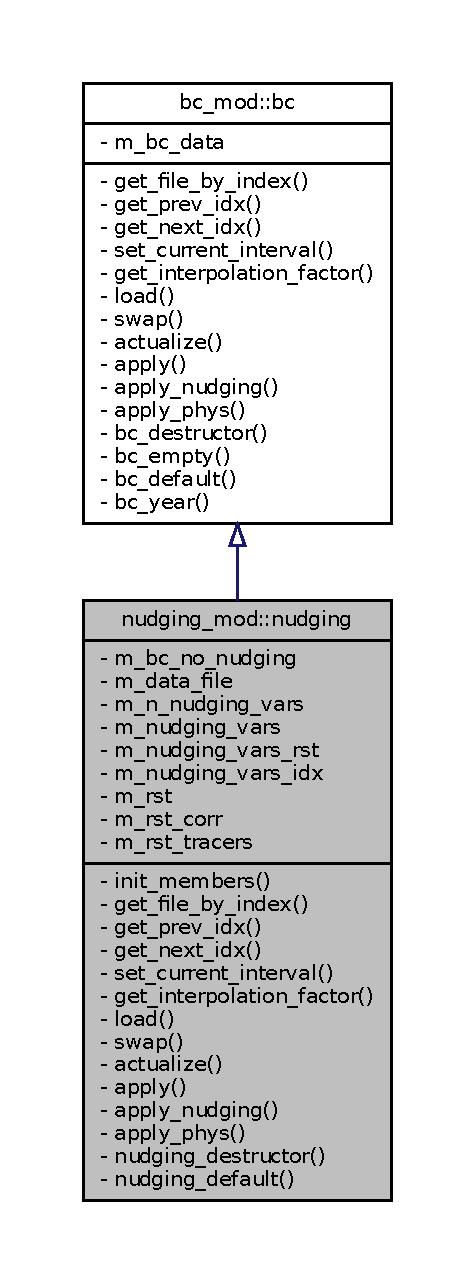
\includegraphics[height=550pt]{structnudging__mod_1_1nudging__inherit__graph}
\end{center}
\end{figure}
\subsubsection*{Private Member Functions}
\begin{DoxyCompactItemize}
\item 
procedure \mbox{\hyperlink{structnudging__mod_1_1nudging_a9c40d1ef319d93b1d60b9d9753cc2acc}{init\+\_\+members}}
\item 
procedure \mbox{\hyperlink{structnudging__mod_1_1nudging_a76b1b1b5a273bab2e43348de8c7721c6}{get\+\_\+file\+\_\+by\+\_\+index}}
\item 
procedure \mbox{\hyperlink{structnudging__mod_1_1nudging_ad1d7271784597d454bc97108232613cd}{get\+\_\+prev\+\_\+idx}}
\item 
procedure \mbox{\hyperlink{structnudging__mod_1_1nudging_afd2889fe6e9aa9560ebb2358efba4dec}{get\+\_\+next\+\_\+idx}}
\item 
procedure \mbox{\hyperlink{structnudging__mod_1_1nudging_ab17fe87aa8dc77bd4bf0cba14d68969a}{set\+\_\+current\+\_\+interval}}
\item 
procedure \mbox{\hyperlink{structnudging__mod_1_1nudging_a55ee89e52a1b3b98d4ff84802f888dd4}{get\+\_\+interpolation\+\_\+factor}}
\item 
procedure \mbox{\hyperlink{structnudging__mod_1_1nudging_ad0fe3f6011636572c0641ef4b01bba33}{load}}
\item 
procedure \mbox{\hyperlink{structnudging__mod_1_1nudging_a9015b684c729f54ba0fe1abc15b28a49}{swap}}
\item 
procedure \mbox{\hyperlink{structnudging__mod_1_1nudging_ade178a579111036782c7b4570018f0d5}{actualize}}
\item 
procedure \mbox{\hyperlink{structnudging__mod_1_1nudging_ad5101760abbec7a50024ecc3435eda49}{apply}}
\item 
procedure \mbox{\hyperlink{structnudging__mod_1_1nudging_a232a6666abdc760493681d65cf8eb8e0}{apply\+\_\+nudging}}
\item 
procedure \mbox{\hyperlink{structnudging__mod_1_1nudging_a5e52b19bbb3e3481ebaa885040e92802}{apply\+\_\+phys}}
\item 
procedure \mbox{\hyperlink{structnudging__mod_1_1nudging_a4b48102a07133bda1873e536608761c7}{nudging\+\_\+destructor}}
\item 
type(\mbox{\hyperlink{structnudging__mod_1_1nudging}{nudging}}) function \mbox{\hyperlink{structnudging__mod_1_1nudging_acaf21e922a461f11284728958f8b2897}{nudging\+\_\+default}} (bc\+\_\+no\+\_\+nudging, data\+\_\+file, n\+\_\+vars, vars, vars\+\_\+idx, rst\+\_\+corr, n\+\_\+tracers)
\end{DoxyCompactItemize}
\subsubsection*{Private Attributes}
\begin{DoxyCompactItemize}
\item 
class(\mbox{\hyperlink{structbc__mod_1_1bc}{bc}}), pointer \mbox{\hyperlink{structnudging__mod_1_1nudging_a07ce30551ce62c0cfebc1a58f1eb3505}{m\+\_\+bc\+\_\+no\+\_\+nudging}} =$>$ null()
\item 
character(len=11) \mbox{\hyperlink{structnudging__mod_1_1nudging_a11b6f9de7a9016ea2e0d6bda207283e7}{m\+\_\+data\+\_\+file}}
\item 
integer \mbox{\hyperlink{structnudging__mod_1_1nudging_a955cb9db8203eea771bcc84337749479}{m\+\_\+n\+\_\+nudging\+\_\+vars}}
\item 
character(len=3), dimension(\+:), allocatable \mbox{\hyperlink{structnudging__mod_1_1nudging_a950f514cbfd66b5cb026e5cff2102237}{m\+\_\+nudging\+\_\+vars}}
\item 
character(len=5), dimension(\+:), allocatable \mbox{\hyperlink{structnudging__mod_1_1nudging_a6a6dc13291b73ea301df0029f4119e32}{m\+\_\+nudging\+\_\+vars\+\_\+rst}}
\item 
integer(4), dimension(\+:), allocatable \mbox{\hyperlink{structnudging__mod_1_1nudging_ac0db1fedd6bbda8fec4467aa3fe62f9b}{m\+\_\+nudging\+\_\+vars\+\_\+idx}}
\item 
double precision, dimension(\+:, \+:, \+:, \+:), allocatable \mbox{\hyperlink{structnudging__mod_1_1nudging_a43dce8fb2e392f219ebc72b28c132275}{m\+\_\+rst}}
\item 
double precision, dimension(\+:), allocatable \mbox{\hyperlink{structnudging__mod_1_1nudging_a288c57246c5970dcc1a0792820841383}{m\+\_\+rst\+\_\+corr}}
\item 
double precision, dimension(\+:, \+:, \+:, \+:), allocatable \mbox{\hyperlink{structnudging__mod_1_1nudging_a3b5a939200dee21d8897f48a44d1454a}{m\+\_\+rst\+\_\+tracers}}
\end{DoxyCompactItemize}


\subsubsection{Member Function/\+Subroutine Documentation}
\mbox{\Hypertarget{structnudging__mod_1_1nudging_ade178a579111036782c7b4570018f0d5}\label{structnudging__mod_1_1nudging_ade178a579111036782c7b4570018f0d5}} 
\index{nudging\+\_\+mod\+::nudging@{nudging\+\_\+mod\+::nudging}!actualize@{actualize}}
\index{actualize@{actualize}!nudging\+\_\+mod\+::nudging@{nudging\+\_\+mod\+::nudging}}
\paragraph{\texorpdfstring{actualize()}{actualize()}}
{\footnotesize\ttfamily procedure nudging\+\_\+mod\+::nudging\+::actualize (\begin{DoxyParamCaption}{ }\end{DoxyParamCaption})\hspace{0.3cm}{\ttfamily [private]}}



Implements \mbox{\hyperlink{structbc__mod_1_1bc_a15503494f181d4090774d948cecdce48}{bc\+\_\+mod\+::bc}}.

\mbox{\Hypertarget{structnudging__mod_1_1nudging_ad5101760abbec7a50024ecc3435eda49}\label{structnudging__mod_1_1nudging_ad5101760abbec7a50024ecc3435eda49}} 
\index{nudging\+\_\+mod\+::nudging@{nudging\+\_\+mod\+::nudging}!apply@{apply}}
\index{apply@{apply}!nudging\+\_\+mod\+::nudging@{nudging\+\_\+mod\+::nudging}}
\paragraph{\texorpdfstring{apply()}{apply()}}
{\footnotesize\ttfamily procedure nudging\+\_\+mod\+::nudging\+::apply (\begin{DoxyParamCaption}{ }\end{DoxyParamCaption})\hspace{0.3cm}{\ttfamily [private]}}



Implements \mbox{\hyperlink{structbc__mod_1_1bc_a628eafc79842d1d1d62e043aedf49aa0}{bc\+\_\+mod\+::bc}}.

\mbox{\Hypertarget{structnudging__mod_1_1nudging_a232a6666abdc760493681d65cf8eb8e0}\label{structnudging__mod_1_1nudging_a232a6666abdc760493681d65cf8eb8e0}} 
\index{nudging\+\_\+mod\+::nudging@{nudging\+\_\+mod\+::nudging}!apply\+\_\+nudging@{apply\+\_\+nudging}}
\index{apply\+\_\+nudging@{apply\+\_\+nudging}!nudging\+\_\+mod\+::nudging@{nudging\+\_\+mod\+::nudging}}
\paragraph{\texorpdfstring{apply\+\_\+nudging()}{apply\_nudging()}}
{\footnotesize\ttfamily procedure nudging\+\_\+mod\+::nudging\+::apply\+\_\+nudging (\begin{DoxyParamCaption}{ }\end{DoxyParamCaption})\hspace{0.3cm}{\ttfamily [private]}}



Implements \mbox{\hyperlink{structbc__mod_1_1bc_a42dc448ba9e50fbb6b1acf03b0d121f3}{bc\+\_\+mod\+::bc}}.

\mbox{\Hypertarget{structnudging__mod_1_1nudging_a5e52b19bbb3e3481ebaa885040e92802}\label{structnudging__mod_1_1nudging_a5e52b19bbb3e3481ebaa885040e92802}} 
\index{nudging\+\_\+mod\+::nudging@{nudging\+\_\+mod\+::nudging}!apply\+\_\+phys@{apply\+\_\+phys}}
\index{apply\+\_\+phys@{apply\+\_\+phys}!nudging\+\_\+mod\+::nudging@{nudging\+\_\+mod\+::nudging}}
\paragraph{\texorpdfstring{apply\+\_\+phys()}{apply\_phys()}}
{\footnotesize\ttfamily procedure nudging\+\_\+mod\+::nudging\+::apply\+\_\+phys (\begin{DoxyParamCaption}{ }\end{DoxyParamCaption})\hspace{0.3cm}{\ttfamily [private]}}



Implements \mbox{\hyperlink{structbc__mod_1_1bc_ad0d03ece320569369a296ff3d4cf10d2}{bc\+\_\+mod\+::bc}}.

\mbox{\Hypertarget{structnudging__mod_1_1nudging_a76b1b1b5a273bab2e43348de8c7721c6}\label{structnudging__mod_1_1nudging_a76b1b1b5a273bab2e43348de8c7721c6}} 
\index{nudging\+\_\+mod\+::nudging@{nudging\+\_\+mod\+::nudging}!get\+\_\+file\+\_\+by\+\_\+index@{get\+\_\+file\+\_\+by\+\_\+index}}
\index{get\+\_\+file\+\_\+by\+\_\+index@{get\+\_\+file\+\_\+by\+\_\+index}!nudging\+\_\+mod\+::nudging@{nudging\+\_\+mod\+::nudging}}
\paragraph{\texorpdfstring{get\+\_\+file\+\_\+by\+\_\+index()}{get\_file\_by\_index()}}
{\footnotesize\ttfamily procedure nudging\+\_\+mod\+::nudging\+::get\+\_\+file\+\_\+by\+\_\+index (\begin{DoxyParamCaption}{ }\end{DoxyParamCaption})\hspace{0.3cm}{\ttfamily [private]}}



Implements \mbox{\hyperlink{structbc__mod_1_1bc_aad031a20982832747243dc3e3fbfce20}{bc\+\_\+mod\+::bc}}.

\mbox{\Hypertarget{structnudging__mod_1_1nudging_a55ee89e52a1b3b98d4ff84802f888dd4}\label{structnudging__mod_1_1nudging_a55ee89e52a1b3b98d4ff84802f888dd4}} 
\index{nudging\+\_\+mod\+::nudging@{nudging\+\_\+mod\+::nudging}!get\+\_\+interpolation\+\_\+factor@{get\+\_\+interpolation\+\_\+factor}}
\index{get\+\_\+interpolation\+\_\+factor@{get\+\_\+interpolation\+\_\+factor}!nudging\+\_\+mod\+::nudging@{nudging\+\_\+mod\+::nudging}}
\paragraph{\texorpdfstring{get\+\_\+interpolation\+\_\+factor()}{get\_interpolation\_factor()}}
{\footnotesize\ttfamily procedure nudging\+\_\+mod\+::nudging\+::get\+\_\+interpolation\+\_\+factor (\begin{DoxyParamCaption}{ }\end{DoxyParamCaption})\hspace{0.3cm}{\ttfamily [private]}}



Implements \mbox{\hyperlink{structbc__mod_1_1bc_a1d7f33a1fd0c18e5ce50af4690c82846}{bc\+\_\+mod\+::bc}}.

\mbox{\Hypertarget{structnudging__mod_1_1nudging_afd2889fe6e9aa9560ebb2358efba4dec}\label{structnudging__mod_1_1nudging_afd2889fe6e9aa9560ebb2358efba4dec}} 
\index{nudging\+\_\+mod\+::nudging@{nudging\+\_\+mod\+::nudging}!get\+\_\+next\+\_\+idx@{get\+\_\+next\+\_\+idx}}
\index{get\+\_\+next\+\_\+idx@{get\+\_\+next\+\_\+idx}!nudging\+\_\+mod\+::nudging@{nudging\+\_\+mod\+::nudging}}
\paragraph{\texorpdfstring{get\+\_\+next\+\_\+idx()}{get\_next\_idx()}}
{\footnotesize\ttfamily procedure nudging\+\_\+mod\+::nudging\+::get\+\_\+next\+\_\+idx (\begin{DoxyParamCaption}{ }\end{DoxyParamCaption})\hspace{0.3cm}{\ttfamily [private]}}



Implements \mbox{\hyperlink{structbc__mod_1_1bc_abf0c1a16ec610ce08ed379315afc7f55}{bc\+\_\+mod\+::bc}}.

\mbox{\Hypertarget{structnudging__mod_1_1nudging_ad1d7271784597d454bc97108232613cd}\label{structnudging__mod_1_1nudging_ad1d7271784597d454bc97108232613cd}} 
\index{nudging\+\_\+mod\+::nudging@{nudging\+\_\+mod\+::nudging}!get\+\_\+prev\+\_\+idx@{get\+\_\+prev\+\_\+idx}}
\index{get\+\_\+prev\+\_\+idx@{get\+\_\+prev\+\_\+idx}!nudging\+\_\+mod\+::nudging@{nudging\+\_\+mod\+::nudging}}
\paragraph{\texorpdfstring{get\+\_\+prev\+\_\+idx()}{get\_prev\_idx()}}
{\footnotesize\ttfamily procedure nudging\+\_\+mod\+::nudging\+::get\+\_\+prev\+\_\+idx (\begin{DoxyParamCaption}{ }\end{DoxyParamCaption})\hspace{0.3cm}{\ttfamily [private]}}



Implements \mbox{\hyperlink{structbc__mod_1_1bc_aa04b9a462194855b7c9111fe67456f0d}{bc\+\_\+mod\+::bc}}.

\mbox{\Hypertarget{structnudging__mod_1_1nudging_a9c40d1ef319d93b1d60b9d9753cc2acc}\label{structnudging__mod_1_1nudging_a9c40d1ef319d93b1d60b9d9753cc2acc}} 
\index{nudging\+\_\+mod\+::nudging@{nudging\+\_\+mod\+::nudging}!init\+\_\+members@{init\+\_\+members}}
\index{init\+\_\+members@{init\+\_\+members}!nudging\+\_\+mod\+::nudging@{nudging\+\_\+mod\+::nudging}}
\paragraph{\texorpdfstring{init\+\_\+members()}{init\_members()}}
{\footnotesize\ttfamily procedure nudging\+\_\+mod\+::nudging\+::init\+\_\+members (\begin{DoxyParamCaption}{ }\end{DoxyParamCaption})\hspace{0.3cm}{\ttfamily [private]}}

\mbox{\Hypertarget{structnudging__mod_1_1nudging_ad0fe3f6011636572c0641ef4b01bba33}\label{structnudging__mod_1_1nudging_ad0fe3f6011636572c0641ef4b01bba33}} 
\index{nudging\+\_\+mod\+::nudging@{nudging\+\_\+mod\+::nudging}!load@{load}}
\index{load@{load}!nudging\+\_\+mod\+::nudging@{nudging\+\_\+mod\+::nudging}}
\paragraph{\texorpdfstring{load()}{load()}}
{\footnotesize\ttfamily procedure nudging\+\_\+mod\+::nudging\+::load (\begin{DoxyParamCaption}{ }\end{DoxyParamCaption})\hspace{0.3cm}{\ttfamily [private]}}



Implements \mbox{\hyperlink{structbc__mod_1_1bc_a1c4ee986270f18f4400c4554c06c5f7b}{bc\+\_\+mod\+::bc}}.

\mbox{\Hypertarget{structnudging__mod_1_1nudging_acaf21e922a461f11284728958f8b2897}\label{structnudging__mod_1_1nudging_acaf21e922a461f11284728958f8b2897}} 
\index{nudging\+\_\+mod\+::nudging@{nudging\+\_\+mod\+::nudging}!nudging\+\_\+default@{nudging\+\_\+default}}
\index{nudging\+\_\+default@{nudging\+\_\+default}!nudging\+\_\+mod\+::nudging@{nudging\+\_\+mod\+::nudging}}
\paragraph{\texorpdfstring{nudging\+\_\+default()}{nudging\_default()}}
{\footnotesize\ttfamily type(\mbox{\hyperlink{structnudging__mod_1_1nudging}{nudging}}) function nudging\+\_\+mod\+::nudging\+::nudging\+\_\+default (\begin{DoxyParamCaption}\item[{class(\mbox{\hyperlink{structbc__mod_1_1bc}{bc}}), intent(in), target}]{bc\+\_\+no\+\_\+nudging,  }\item[{character(len=11), intent(in)}]{data\+\_\+file,  }\item[{integer, intent(in)}]{n\+\_\+vars,  }\item[{character(len=27), intent(in)}]{vars,  }\item[{integer(4), dimension(n\+\_\+vars), intent(in)}]{vars\+\_\+idx,  }\item[{double precision, dimension(n\+\_\+vars), intent(in)}]{rst\+\_\+corr,  }\item[{integer, intent(in)}]{n\+\_\+tracers }\end{DoxyParamCaption})\hspace{0.3cm}{\ttfamily [private]}}

\mbox{\Hypertarget{structnudging__mod_1_1nudging_a4b48102a07133bda1873e536608761c7}\label{structnudging__mod_1_1nudging_a4b48102a07133bda1873e536608761c7}} 
\index{nudging\+\_\+mod\+::nudging@{nudging\+\_\+mod\+::nudging}!nudging\+\_\+destructor@{nudging\+\_\+destructor}}
\index{nudging\+\_\+destructor@{nudging\+\_\+destructor}!nudging\+\_\+mod\+::nudging@{nudging\+\_\+mod\+::nudging}}
\paragraph{\texorpdfstring{nudging\+\_\+destructor()}{nudging\_destructor()}}
{\footnotesize\ttfamily procedure nudging\+\_\+mod\+::nudging\+::nudging\+\_\+destructor (\begin{DoxyParamCaption}{ }\end{DoxyParamCaption})\hspace{0.3cm}{\ttfamily [private]}}

\mbox{\Hypertarget{structnudging__mod_1_1nudging_ab17fe87aa8dc77bd4bf0cba14d68969a}\label{structnudging__mod_1_1nudging_ab17fe87aa8dc77bd4bf0cba14d68969a}} 
\index{nudging\+\_\+mod\+::nudging@{nudging\+\_\+mod\+::nudging}!set\+\_\+current\+\_\+interval@{set\+\_\+current\+\_\+interval}}
\index{set\+\_\+current\+\_\+interval@{set\+\_\+current\+\_\+interval}!nudging\+\_\+mod\+::nudging@{nudging\+\_\+mod\+::nudging}}
\paragraph{\texorpdfstring{set\+\_\+current\+\_\+interval()}{set\_current\_interval()}}
{\footnotesize\ttfamily procedure nudging\+\_\+mod\+::nudging\+::set\+\_\+current\+\_\+interval (\begin{DoxyParamCaption}{ }\end{DoxyParamCaption})\hspace{0.3cm}{\ttfamily [private]}}



Implements \mbox{\hyperlink{structbc__mod_1_1bc_adf9262a425534bd18d98809381034ca1}{bc\+\_\+mod\+::bc}}.

\mbox{\Hypertarget{structnudging__mod_1_1nudging_a9015b684c729f54ba0fe1abc15b28a49}\label{structnudging__mod_1_1nudging_a9015b684c729f54ba0fe1abc15b28a49}} 
\index{nudging\+\_\+mod\+::nudging@{nudging\+\_\+mod\+::nudging}!swap@{swap}}
\index{swap@{swap}!nudging\+\_\+mod\+::nudging@{nudging\+\_\+mod\+::nudging}}
\paragraph{\texorpdfstring{swap()}{swap()}}
{\footnotesize\ttfamily procedure nudging\+\_\+mod\+::nudging\+::swap (\begin{DoxyParamCaption}{ }\end{DoxyParamCaption})\hspace{0.3cm}{\ttfamily [private]}}



Implements \mbox{\hyperlink{structbc__mod_1_1bc_a925ae5960dbfc854eab908c52c13f719}{bc\+\_\+mod\+::bc}}.



\subsubsection{Member Data Documentation}
\mbox{\Hypertarget{structnudging__mod_1_1nudging_a07ce30551ce62c0cfebc1a58f1eb3505}\label{structnudging__mod_1_1nudging_a07ce30551ce62c0cfebc1a58f1eb3505}} 
\index{nudging\+\_\+mod\+::nudging@{nudging\+\_\+mod\+::nudging}!m\+\_\+bc\+\_\+no\+\_\+nudging@{m\+\_\+bc\+\_\+no\+\_\+nudging}}
\index{m\+\_\+bc\+\_\+no\+\_\+nudging@{m\+\_\+bc\+\_\+no\+\_\+nudging}!nudging\+\_\+mod\+::nudging@{nudging\+\_\+mod\+::nudging}}
\paragraph{\texorpdfstring{m\+\_\+bc\+\_\+no\+\_\+nudging}{m\_bc\_no\_nudging}}
{\footnotesize\ttfamily class(\mbox{\hyperlink{structbc__mod_1_1bc}{bc}}), pointer nudging\+\_\+mod\+::nudging\+::m\+\_\+bc\+\_\+no\+\_\+nudging =$>$ null()\hspace{0.3cm}{\ttfamily [private]}}

\mbox{\Hypertarget{structnudging__mod_1_1nudging_a11b6f9de7a9016ea2e0d6bda207283e7}\label{structnudging__mod_1_1nudging_a11b6f9de7a9016ea2e0d6bda207283e7}} 
\index{nudging\+\_\+mod\+::nudging@{nudging\+\_\+mod\+::nudging}!m\+\_\+data\+\_\+file@{m\+\_\+data\+\_\+file}}
\index{m\+\_\+data\+\_\+file@{m\+\_\+data\+\_\+file}!nudging\+\_\+mod\+::nudging@{nudging\+\_\+mod\+::nudging}}
\paragraph{\texorpdfstring{m\+\_\+data\+\_\+file}{m\_data\_file}}
{\footnotesize\ttfamily character(len=11) nudging\+\_\+mod\+::nudging\+::m\+\_\+data\+\_\+file\hspace{0.3cm}{\ttfamily [private]}}

\mbox{\Hypertarget{structnudging__mod_1_1nudging_a955cb9db8203eea771bcc84337749479}\label{structnudging__mod_1_1nudging_a955cb9db8203eea771bcc84337749479}} 
\index{nudging\+\_\+mod\+::nudging@{nudging\+\_\+mod\+::nudging}!m\+\_\+n\+\_\+nudging\+\_\+vars@{m\+\_\+n\+\_\+nudging\+\_\+vars}}
\index{m\+\_\+n\+\_\+nudging\+\_\+vars@{m\+\_\+n\+\_\+nudging\+\_\+vars}!nudging\+\_\+mod\+::nudging@{nudging\+\_\+mod\+::nudging}}
\paragraph{\texorpdfstring{m\+\_\+n\+\_\+nudging\+\_\+vars}{m\_n\_nudging\_vars}}
{\footnotesize\ttfamily integer nudging\+\_\+mod\+::nudging\+::m\+\_\+n\+\_\+nudging\+\_\+vars\hspace{0.3cm}{\ttfamily [private]}}

\mbox{\Hypertarget{structnudging__mod_1_1nudging_a950f514cbfd66b5cb026e5cff2102237}\label{structnudging__mod_1_1nudging_a950f514cbfd66b5cb026e5cff2102237}} 
\index{nudging\+\_\+mod\+::nudging@{nudging\+\_\+mod\+::nudging}!m\+\_\+nudging\+\_\+vars@{m\+\_\+nudging\+\_\+vars}}
\index{m\+\_\+nudging\+\_\+vars@{m\+\_\+nudging\+\_\+vars}!nudging\+\_\+mod\+::nudging@{nudging\+\_\+mod\+::nudging}}
\paragraph{\texorpdfstring{m\+\_\+nudging\+\_\+vars}{m\_nudging\_vars}}
{\footnotesize\ttfamily character(len=3), dimension(\+:), allocatable nudging\+\_\+mod\+::nudging\+::m\+\_\+nudging\+\_\+vars\hspace{0.3cm}{\ttfamily [private]}}

\mbox{\Hypertarget{structnudging__mod_1_1nudging_ac0db1fedd6bbda8fec4467aa3fe62f9b}\label{structnudging__mod_1_1nudging_ac0db1fedd6bbda8fec4467aa3fe62f9b}} 
\index{nudging\+\_\+mod\+::nudging@{nudging\+\_\+mod\+::nudging}!m\+\_\+nudging\+\_\+vars\+\_\+idx@{m\+\_\+nudging\+\_\+vars\+\_\+idx}}
\index{m\+\_\+nudging\+\_\+vars\+\_\+idx@{m\+\_\+nudging\+\_\+vars\+\_\+idx}!nudging\+\_\+mod\+::nudging@{nudging\+\_\+mod\+::nudging}}
\paragraph{\texorpdfstring{m\+\_\+nudging\+\_\+vars\+\_\+idx}{m\_nudging\_vars\_idx}}
{\footnotesize\ttfamily integer(4), dimension(\+:), allocatable nudging\+\_\+mod\+::nudging\+::m\+\_\+nudging\+\_\+vars\+\_\+idx\hspace{0.3cm}{\ttfamily [private]}}

\mbox{\Hypertarget{structnudging__mod_1_1nudging_a6a6dc13291b73ea301df0029f4119e32}\label{structnudging__mod_1_1nudging_a6a6dc13291b73ea301df0029f4119e32}} 
\index{nudging\+\_\+mod\+::nudging@{nudging\+\_\+mod\+::nudging}!m\+\_\+nudging\+\_\+vars\+\_\+rst@{m\+\_\+nudging\+\_\+vars\+\_\+rst}}
\index{m\+\_\+nudging\+\_\+vars\+\_\+rst@{m\+\_\+nudging\+\_\+vars\+\_\+rst}!nudging\+\_\+mod\+::nudging@{nudging\+\_\+mod\+::nudging}}
\paragraph{\texorpdfstring{m\+\_\+nudging\+\_\+vars\+\_\+rst}{m\_nudging\_vars\_rst}}
{\footnotesize\ttfamily character(len=5), dimension(\+:), allocatable nudging\+\_\+mod\+::nudging\+::m\+\_\+nudging\+\_\+vars\+\_\+rst\hspace{0.3cm}{\ttfamily [private]}}

\mbox{\Hypertarget{structnudging__mod_1_1nudging_a43dce8fb2e392f219ebc72b28c132275}\label{structnudging__mod_1_1nudging_a43dce8fb2e392f219ebc72b28c132275}} 
\index{nudging\+\_\+mod\+::nudging@{nudging\+\_\+mod\+::nudging}!m\+\_\+rst@{m\+\_\+rst}}
\index{m\+\_\+rst@{m\+\_\+rst}!nudging\+\_\+mod\+::nudging@{nudging\+\_\+mod\+::nudging}}
\paragraph{\texorpdfstring{m\+\_\+rst}{m\_rst}}
{\footnotesize\ttfamily double precision, dimension(\+:, \+:, \+:, \+:), allocatable nudging\+\_\+mod\+::nudging\+::m\+\_\+rst\hspace{0.3cm}{\ttfamily [private]}}

\mbox{\Hypertarget{structnudging__mod_1_1nudging_a288c57246c5970dcc1a0792820841383}\label{structnudging__mod_1_1nudging_a288c57246c5970dcc1a0792820841383}} 
\index{nudging\+\_\+mod\+::nudging@{nudging\+\_\+mod\+::nudging}!m\+\_\+rst\+\_\+corr@{m\+\_\+rst\+\_\+corr}}
\index{m\+\_\+rst\+\_\+corr@{m\+\_\+rst\+\_\+corr}!nudging\+\_\+mod\+::nudging@{nudging\+\_\+mod\+::nudging}}
\paragraph{\texorpdfstring{m\+\_\+rst\+\_\+corr}{m\_rst\_corr}}
{\footnotesize\ttfamily double precision, dimension(\+:), allocatable nudging\+\_\+mod\+::nudging\+::m\+\_\+rst\+\_\+corr\hspace{0.3cm}{\ttfamily [private]}}

\mbox{\Hypertarget{structnudging__mod_1_1nudging_a3b5a939200dee21d8897f48a44d1454a}\label{structnudging__mod_1_1nudging_a3b5a939200dee21d8897f48a44d1454a}} 
\index{nudging\+\_\+mod\+::nudging@{nudging\+\_\+mod\+::nudging}!m\+\_\+rst\+\_\+tracers@{m\+\_\+rst\+\_\+tracers}}
\index{m\+\_\+rst\+\_\+tracers@{m\+\_\+rst\+\_\+tracers}!nudging\+\_\+mod\+::nudging@{nudging\+\_\+mod\+::nudging}}
\paragraph{\texorpdfstring{m\+\_\+rst\+\_\+tracers}{m\_rst\_tracers}}
{\footnotesize\ttfamily double precision, dimension(\+:, \+:, \+:, \+:), allocatable nudging\+\_\+mod\+::nudging\+::m\+\_\+rst\+\_\+tracers\hspace{0.3cm}{\ttfamily [private]}}


\hypertarget{structrivers__mod_1_1rivers}{}\subsection{rivers\+\_\+mod\+:\+:rivers Interface Reference}
\label{structrivers__mod_1_1rivers}\index{rivers\+\_\+mod\+::rivers@{rivers\+\_\+mod\+::rivers}}


Inheritance diagram for rivers\+\_\+mod\+:\+:rivers\+:
\nopagebreak
\begin{figure}[H]
\begin{center}
\leavevmode
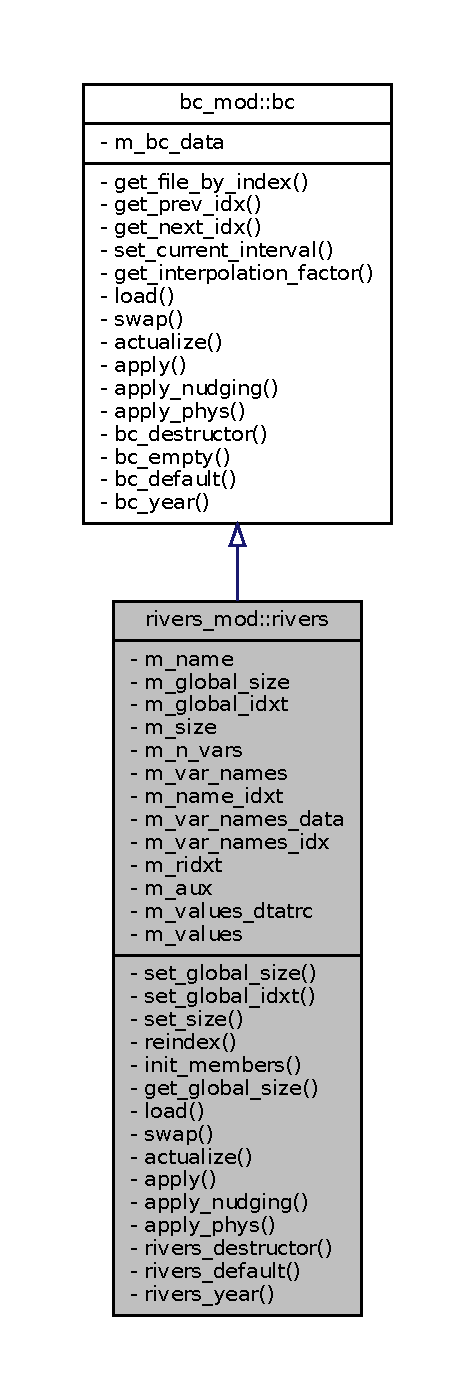
\includegraphics[height=550pt]{structrivers__mod_1_1rivers__inherit__graph}
\end{center}
\end{figure}
\subsubsection*{Private Member Functions}
\begin{DoxyCompactItemize}
\item 
procedure \mbox{\hyperlink{structrivers__mod_1_1rivers_a47e4b220c2eaf84a5ddbddd2c504f3c7}{set\+\_\+global\+\_\+size}}
\item 
procedure \mbox{\hyperlink{structrivers__mod_1_1rivers_a378a92f6f66820ec146e52b2c55803fc}{set\+\_\+global\+\_\+idxt}}
\item 
procedure \mbox{\hyperlink{structrivers__mod_1_1rivers_ae1f9392fa0882bffb1d45f802ad23a8d}{set\+\_\+size}}
\item 
procedure \mbox{\hyperlink{structrivers__mod_1_1rivers_a0c86ef831afa277f36aaef42d9e9ac4b}{reindex}}
\item 
procedure \mbox{\hyperlink{structrivers__mod_1_1rivers_a3ff0321c021f612d772817edbb872e37}{init\+\_\+members}}
\item 
procedure \mbox{\hyperlink{structrivers__mod_1_1rivers_a51f0caa3611caf9a391fe5797f46c031}{get\+\_\+global\+\_\+size}}
\item 
procedure \mbox{\hyperlink{structrivers__mod_1_1rivers_a4eac45372772ea12c7f18505a4de53ee}{load}}
\item 
procedure \mbox{\hyperlink{structrivers__mod_1_1rivers_a7bcfc95d699f097aed2975941cabe059}{swap}}
\item 
procedure \mbox{\hyperlink{structrivers__mod_1_1rivers_a7c1b4c7a383553f4cacdae90725f3249}{actualize}}
\item 
procedure \mbox{\hyperlink{structrivers__mod_1_1rivers_a97eb13e48a07c9020cb1b353d42a5466}{apply}}
\item 
procedure \mbox{\hyperlink{structrivers__mod_1_1rivers_aaa8c35a085317190f69e097caba60cfb}{apply\+\_\+nudging}}
\item 
procedure \mbox{\hyperlink{structrivers__mod_1_1rivers_a4f6360b228319a4189289cafc2e3fd74}{apply\+\_\+phys}}
\item 
procedure \mbox{\hyperlink{structrivers__mod_1_1rivers_a172c1ec96e9bd79a6a2ec289193068aa}{rivers\+\_\+destructor}}
\item 
type(\mbox{\hyperlink{structrivers__mod_1_1rivers}{rivers}}) function \mbox{\hyperlink{structrivers__mod_1_1rivers_a6ba78d48f5759b9bdf70beaaa958a0ce}{rivers\+\_\+default}} (files\+\_\+namelist, bc\+\_\+name, n\+\_\+vars, vars, var\+\_\+names\+\_\+idx)
\item 
type(\mbox{\hyperlink{structrivers__mod_1_1rivers}{rivers}}) function \mbox{\hyperlink{structrivers__mod_1_1rivers_ac4628566baa63304f7cb53f5935ddaee}{rivers\+\_\+year}} (files\+\_\+namelist, bc\+\_\+name, n\+\_\+vars, vars, var\+\_\+names\+\_\+idx, start\+\_\+time\+\_\+string, end\+\_\+time\+\_\+string)
\end{DoxyCompactItemize}
\subsubsection*{Private Attributes}
\begin{DoxyCompactItemize}
\item 
character(len=3) \mbox{\hyperlink{structrivers__mod_1_1rivers_a421cdf84127a4dd69eff780d41170b3d}{m\+\_\+name}}
\item 
integer(4) \mbox{\hyperlink{structrivers__mod_1_1rivers_af71ac049d12dcd8a69adbac0e7b09134}{m\+\_\+global\+\_\+size}}
\item 
integer(4), dimension(\+:), allocatable \mbox{\hyperlink{structrivers__mod_1_1rivers_acd095de754fae3344e723d899335cba6}{m\+\_\+global\+\_\+idxt}}
\item 
integer(4) \mbox{\hyperlink{structrivers__mod_1_1rivers_acbec48622693bfb1b79cce4b90718e7d}{m\+\_\+size}}
\item 
integer \mbox{\hyperlink{structrivers__mod_1_1rivers_aa6f2afd13aef94d33f271874ad5c4f46}{m\+\_\+n\+\_\+vars}}
\item 
character(len=3), dimension(\+:), allocatable \mbox{\hyperlink{structrivers__mod_1_1rivers_ac0d31c21015866224b4124937901ffe7}{m\+\_\+var\+\_\+names}}
\item 
character(len=12) \mbox{\hyperlink{structrivers__mod_1_1rivers_a60422ea3260a9cd75931b5eaf65ba314}{m\+\_\+name\+\_\+idxt}}
\item 
character(len=7), dimension(\+:), allocatable \mbox{\hyperlink{structrivers__mod_1_1rivers_a48be3643f87dce758d6a72992fa129ae}{m\+\_\+var\+\_\+names\+\_\+data}}
\item 
integer(4), dimension(\+:), allocatable \mbox{\hyperlink{structrivers__mod_1_1rivers_a64986ca8554b5250658d7cf7b97218fb}{m\+\_\+var\+\_\+names\+\_\+idx}}
\item 
integer(4), dimension(\+:, \+:), allocatable \mbox{\hyperlink{structrivers__mod_1_1rivers_adbf8adce081563e1dff036ed90baa3ef}{m\+\_\+ridxt}}
\item 
double precision, dimension(\+:), allocatable \mbox{\hyperlink{structrivers__mod_1_1rivers_abf7afd67f998abeb46cdc4f91b460bc3}{m\+\_\+aux}}
\item 
double precision, dimension(\+:, \+:, \+:), allocatable \mbox{\hyperlink{structrivers__mod_1_1rivers_a75c34142c25f514950b789f5b90ff63b}{m\+\_\+values\+\_\+dtatrc}}
\item 
double precision, dimension(\+:, \+:), allocatable \mbox{\hyperlink{structrivers__mod_1_1rivers_a58530c3fd75177ebe8f2648ad4dccbfc}{m\+\_\+values}}
\end{DoxyCompactItemize}


\subsubsection{Member Function/\+Subroutine Documentation}
\mbox{\Hypertarget{structrivers__mod_1_1rivers_a7c1b4c7a383553f4cacdae90725f3249}\label{structrivers__mod_1_1rivers_a7c1b4c7a383553f4cacdae90725f3249}} 
\index{rivers\+\_\+mod\+::rivers@{rivers\+\_\+mod\+::rivers}!actualize@{actualize}}
\index{actualize@{actualize}!rivers\+\_\+mod\+::rivers@{rivers\+\_\+mod\+::rivers}}
\paragraph{\texorpdfstring{actualize()}{actualize()}}
{\footnotesize\ttfamily procedure rivers\+\_\+mod\+::rivers\+::actualize (\begin{DoxyParamCaption}{ }\end{DoxyParamCaption})\hspace{0.3cm}{\ttfamily [private]}}



Implements \mbox{\hyperlink{structbc__mod_1_1bc_a15503494f181d4090774d948cecdce48}{bc\+\_\+mod\+::bc}}.

\mbox{\Hypertarget{structrivers__mod_1_1rivers_a97eb13e48a07c9020cb1b353d42a5466}\label{structrivers__mod_1_1rivers_a97eb13e48a07c9020cb1b353d42a5466}} 
\index{rivers\+\_\+mod\+::rivers@{rivers\+\_\+mod\+::rivers}!apply@{apply}}
\index{apply@{apply}!rivers\+\_\+mod\+::rivers@{rivers\+\_\+mod\+::rivers}}
\paragraph{\texorpdfstring{apply()}{apply()}}
{\footnotesize\ttfamily procedure rivers\+\_\+mod\+::rivers\+::apply (\begin{DoxyParamCaption}{ }\end{DoxyParamCaption})\hspace{0.3cm}{\ttfamily [private]}}



Implements \mbox{\hyperlink{structbc__mod_1_1bc_a628eafc79842d1d1d62e043aedf49aa0}{bc\+\_\+mod\+::bc}}.

\mbox{\Hypertarget{structrivers__mod_1_1rivers_aaa8c35a085317190f69e097caba60cfb}\label{structrivers__mod_1_1rivers_aaa8c35a085317190f69e097caba60cfb}} 
\index{rivers\+\_\+mod\+::rivers@{rivers\+\_\+mod\+::rivers}!apply\+\_\+nudging@{apply\+\_\+nudging}}
\index{apply\+\_\+nudging@{apply\+\_\+nudging}!rivers\+\_\+mod\+::rivers@{rivers\+\_\+mod\+::rivers}}
\paragraph{\texorpdfstring{apply\+\_\+nudging()}{apply\_nudging()}}
{\footnotesize\ttfamily procedure rivers\+\_\+mod\+::rivers\+::apply\+\_\+nudging (\begin{DoxyParamCaption}{ }\end{DoxyParamCaption})\hspace{0.3cm}{\ttfamily [private]}}



Implements \mbox{\hyperlink{structbc__mod_1_1bc_a42dc448ba9e50fbb6b1acf03b0d121f3}{bc\+\_\+mod\+::bc}}.

\mbox{\Hypertarget{structrivers__mod_1_1rivers_a4f6360b228319a4189289cafc2e3fd74}\label{structrivers__mod_1_1rivers_a4f6360b228319a4189289cafc2e3fd74}} 
\index{rivers\+\_\+mod\+::rivers@{rivers\+\_\+mod\+::rivers}!apply\+\_\+phys@{apply\+\_\+phys}}
\index{apply\+\_\+phys@{apply\+\_\+phys}!rivers\+\_\+mod\+::rivers@{rivers\+\_\+mod\+::rivers}}
\paragraph{\texorpdfstring{apply\+\_\+phys()}{apply\_phys()}}
{\footnotesize\ttfamily procedure rivers\+\_\+mod\+::rivers\+::apply\+\_\+phys (\begin{DoxyParamCaption}{ }\end{DoxyParamCaption})\hspace{0.3cm}{\ttfamily [private]}}



Implements \mbox{\hyperlink{structbc__mod_1_1bc_ad0d03ece320569369a296ff3d4cf10d2}{bc\+\_\+mod\+::bc}}.

\mbox{\Hypertarget{structrivers__mod_1_1rivers_a51f0caa3611caf9a391fe5797f46c031}\label{structrivers__mod_1_1rivers_a51f0caa3611caf9a391fe5797f46c031}} 
\index{rivers\+\_\+mod\+::rivers@{rivers\+\_\+mod\+::rivers}!get\+\_\+global\+\_\+size@{get\+\_\+global\+\_\+size}}
\index{get\+\_\+global\+\_\+size@{get\+\_\+global\+\_\+size}!rivers\+\_\+mod\+::rivers@{rivers\+\_\+mod\+::rivers}}
\paragraph{\texorpdfstring{get\+\_\+global\+\_\+size()}{get\_global\_size()}}
{\footnotesize\ttfamily procedure rivers\+\_\+mod\+::rivers\+::get\+\_\+global\+\_\+size (\begin{DoxyParamCaption}{ }\end{DoxyParamCaption})\hspace{0.3cm}{\ttfamily [private]}}

\mbox{\Hypertarget{structrivers__mod_1_1rivers_a3ff0321c021f612d772817edbb872e37}\label{structrivers__mod_1_1rivers_a3ff0321c021f612d772817edbb872e37}} 
\index{rivers\+\_\+mod\+::rivers@{rivers\+\_\+mod\+::rivers}!init\+\_\+members@{init\+\_\+members}}
\index{init\+\_\+members@{init\+\_\+members}!rivers\+\_\+mod\+::rivers@{rivers\+\_\+mod\+::rivers}}
\paragraph{\texorpdfstring{init\+\_\+members()}{init\_members()}}
{\footnotesize\ttfamily procedure rivers\+\_\+mod\+::rivers\+::init\+\_\+members (\begin{DoxyParamCaption}{ }\end{DoxyParamCaption})\hspace{0.3cm}{\ttfamily [private]}}

\mbox{\Hypertarget{structrivers__mod_1_1rivers_a4eac45372772ea12c7f18505a4de53ee}\label{structrivers__mod_1_1rivers_a4eac45372772ea12c7f18505a4de53ee}} 
\index{rivers\+\_\+mod\+::rivers@{rivers\+\_\+mod\+::rivers}!load@{load}}
\index{load@{load}!rivers\+\_\+mod\+::rivers@{rivers\+\_\+mod\+::rivers}}
\paragraph{\texorpdfstring{load()}{load()}}
{\footnotesize\ttfamily procedure rivers\+\_\+mod\+::rivers\+::load (\begin{DoxyParamCaption}{ }\end{DoxyParamCaption})\hspace{0.3cm}{\ttfamily [private]}}



Implements \mbox{\hyperlink{structbc__mod_1_1bc_a1c4ee986270f18f4400c4554c06c5f7b}{bc\+\_\+mod\+::bc}}.

\mbox{\Hypertarget{structrivers__mod_1_1rivers_a0c86ef831afa277f36aaef42d9e9ac4b}\label{structrivers__mod_1_1rivers_a0c86ef831afa277f36aaef42d9e9ac4b}} 
\index{rivers\+\_\+mod\+::rivers@{rivers\+\_\+mod\+::rivers}!reindex@{reindex}}
\index{reindex@{reindex}!rivers\+\_\+mod\+::rivers@{rivers\+\_\+mod\+::rivers}}
\paragraph{\texorpdfstring{reindex()}{reindex()}}
{\footnotesize\ttfamily procedure rivers\+\_\+mod\+::rivers\+::reindex (\begin{DoxyParamCaption}{ }\end{DoxyParamCaption})\hspace{0.3cm}{\ttfamily [private]}}

\mbox{\Hypertarget{structrivers__mod_1_1rivers_a6ba78d48f5759b9bdf70beaaa958a0ce}\label{structrivers__mod_1_1rivers_a6ba78d48f5759b9bdf70beaaa958a0ce}} 
\index{rivers\+\_\+mod\+::rivers@{rivers\+\_\+mod\+::rivers}!rivers\+\_\+default@{rivers\+\_\+default}}
\index{rivers\+\_\+default@{rivers\+\_\+default}!rivers\+\_\+mod\+::rivers@{rivers\+\_\+mod\+::rivers}}
\paragraph{\texorpdfstring{rivers\+\_\+default()}{rivers\_default()}}
{\footnotesize\ttfamily type(\mbox{\hyperlink{structrivers__mod_1_1rivers}{rivers}}) function rivers\+\_\+mod\+::rivers\+::rivers\+\_\+default (\begin{DoxyParamCaption}\item[{character(len=22), intent(in)}]{files\+\_\+namelist,  }\item[{character(len=3)}]{bc\+\_\+name,  }\item[{integer, intent(in)}]{n\+\_\+vars,  }\item[{character(len=23), intent(in)}]{vars,  }\item[{integer(4), dimension(n\+\_\+vars), intent(in)}]{var\+\_\+names\+\_\+idx }\end{DoxyParamCaption})\hspace{0.3cm}{\ttfamily [private]}}

\mbox{\Hypertarget{structrivers__mod_1_1rivers_a172c1ec96e9bd79a6a2ec289193068aa}\label{structrivers__mod_1_1rivers_a172c1ec96e9bd79a6a2ec289193068aa}} 
\index{rivers\+\_\+mod\+::rivers@{rivers\+\_\+mod\+::rivers}!rivers\+\_\+destructor@{rivers\+\_\+destructor}}
\index{rivers\+\_\+destructor@{rivers\+\_\+destructor}!rivers\+\_\+mod\+::rivers@{rivers\+\_\+mod\+::rivers}}
\paragraph{\texorpdfstring{rivers\+\_\+destructor()}{rivers\_destructor()}}
{\footnotesize\ttfamily procedure rivers\+\_\+mod\+::rivers\+::rivers\+\_\+destructor (\begin{DoxyParamCaption}{ }\end{DoxyParamCaption})\hspace{0.3cm}{\ttfamily [private]}}

\mbox{\Hypertarget{structrivers__mod_1_1rivers_ac4628566baa63304f7cb53f5935ddaee}\label{structrivers__mod_1_1rivers_ac4628566baa63304f7cb53f5935ddaee}} 
\index{rivers\+\_\+mod\+::rivers@{rivers\+\_\+mod\+::rivers}!rivers\+\_\+year@{rivers\+\_\+year}}
\index{rivers\+\_\+year@{rivers\+\_\+year}!rivers\+\_\+mod\+::rivers@{rivers\+\_\+mod\+::rivers}}
\paragraph{\texorpdfstring{rivers\+\_\+year()}{rivers\_year()}}
{\footnotesize\ttfamily type(\mbox{\hyperlink{structrivers__mod_1_1rivers}{rivers}}) function rivers\+\_\+mod\+::rivers\+::rivers\+\_\+year (\begin{DoxyParamCaption}\item[{character(len=27), intent(in)}]{files\+\_\+namelist,  }\item[{character(len=3)}]{bc\+\_\+name,  }\item[{integer, intent(in)}]{n\+\_\+vars,  }\item[{character(len=23), intent(in)}]{vars,  }\item[{integer(4), dimension(n\+\_\+vars), intent(in)}]{var\+\_\+names\+\_\+idx,  }\item[{character(len=17), intent(in)}]{start\+\_\+time\+\_\+string,  }\item[{character(len=17), intent(in)}]{end\+\_\+time\+\_\+string }\end{DoxyParamCaption})\hspace{0.3cm}{\ttfamily [private]}}

\mbox{\Hypertarget{structrivers__mod_1_1rivers_a378a92f6f66820ec146e52b2c55803fc}\label{structrivers__mod_1_1rivers_a378a92f6f66820ec146e52b2c55803fc}} 
\index{rivers\+\_\+mod\+::rivers@{rivers\+\_\+mod\+::rivers}!set\+\_\+global\+\_\+idxt@{set\+\_\+global\+\_\+idxt}}
\index{set\+\_\+global\+\_\+idxt@{set\+\_\+global\+\_\+idxt}!rivers\+\_\+mod\+::rivers@{rivers\+\_\+mod\+::rivers}}
\paragraph{\texorpdfstring{set\+\_\+global\+\_\+idxt()}{set\_global\_idxt()}}
{\footnotesize\ttfamily procedure rivers\+\_\+mod\+::rivers\+::set\+\_\+global\+\_\+idxt (\begin{DoxyParamCaption}{ }\end{DoxyParamCaption})\hspace{0.3cm}{\ttfamily [private]}}

\mbox{\Hypertarget{structrivers__mod_1_1rivers_a47e4b220c2eaf84a5ddbddd2c504f3c7}\label{structrivers__mod_1_1rivers_a47e4b220c2eaf84a5ddbddd2c504f3c7}} 
\index{rivers\+\_\+mod\+::rivers@{rivers\+\_\+mod\+::rivers}!set\+\_\+global\+\_\+size@{set\+\_\+global\+\_\+size}}
\index{set\+\_\+global\+\_\+size@{set\+\_\+global\+\_\+size}!rivers\+\_\+mod\+::rivers@{rivers\+\_\+mod\+::rivers}}
\paragraph{\texorpdfstring{set\+\_\+global\+\_\+size()}{set\_global\_size()}}
{\footnotesize\ttfamily procedure rivers\+\_\+mod\+::rivers\+::set\+\_\+global\+\_\+size (\begin{DoxyParamCaption}{ }\end{DoxyParamCaption})\hspace{0.3cm}{\ttfamily [private]}}

\mbox{\Hypertarget{structrivers__mod_1_1rivers_ae1f9392fa0882bffb1d45f802ad23a8d}\label{structrivers__mod_1_1rivers_ae1f9392fa0882bffb1d45f802ad23a8d}} 
\index{rivers\+\_\+mod\+::rivers@{rivers\+\_\+mod\+::rivers}!set\+\_\+size@{set\+\_\+size}}
\index{set\+\_\+size@{set\+\_\+size}!rivers\+\_\+mod\+::rivers@{rivers\+\_\+mod\+::rivers}}
\paragraph{\texorpdfstring{set\+\_\+size()}{set\_size()}}
{\footnotesize\ttfamily procedure rivers\+\_\+mod\+::rivers\+::set\+\_\+size (\begin{DoxyParamCaption}{ }\end{DoxyParamCaption})\hspace{0.3cm}{\ttfamily [private]}}

\mbox{\Hypertarget{structrivers__mod_1_1rivers_a7bcfc95d699f097aed2975941cabe059}\label{structrivers__mod_1_1rivers_a7bcfc95d699f097aed2975941cabe059}} 
\index{rivers\+\_\+mod\+::rivers@{rivers\+\_\+mod\+::rivers}!swap@{swap}}
\index{swap@{swap}!rivers\+\_\+mod\+::rivers@{rivers\+\_\+mod\+::rivers}}
\paragraph{\texorpdfstring{swap()}{swap()}}
{\footnotesize\ttfamily procedure rivers\+\_\+mod\+::rivers\+::swap (\begin{DoxyParamCaption}{ }\end{DoxyParamCaption})\hspace{0.3cm}{\ttfamily [private]}}



Implements \mbox{\hyperlink{structbc__mod_1_1bc_a925ae5960dbfc854eab908c52c13f719}{bc\+\_\+mod\+::bc}}.



\subsubsection{Member Data Documentation}
\mbox{\Hypertarget{structrivers__mod_1_1rivers_abf7afd67f998abeb46cdc4f91b460bc3}\label{structrivers__mod_1_1rivers_abf7afd67f998abeb46cdc4f91b460bc3}} 
\index{rivers\+\_\+mod\+::rivers@{rivers\+\_\+mod\+::rivers}!m\+\_\+aux@{m\+\_\+aux}}
\index{m\+\_\+aux@{m\+\_\+aux}!rivers\+\_\+mod\+::rivers@{rivers\+\_\+mod\+::rivers}}
\paragraph{\texorpdfstring{m\+\_\+aux}{m\_aux}}
{\footnotesize\ttfamily double precision, dimension(\+:), allocatable rivers\+\_\+mod\+::rivers\+::m\+\_\+aux\hspace{0.3cm}{\ttfamily [private]}}

\mbox{\Hypertarget{structrivers__mod_1_1rivers_acd095de754fae3344e723d899335cba6}\label{structrivers__mod_1_1rivers_acd095de754fae3344e723d899335cba6}} 
\index{rivers\+\_\+mod\+::rivers@{rivers\+\_\+mod\+::rivers}!m\+\_\+global\+\_\+idxt@{m\+\_\+global\+\_\+idxt}}
\index{m\+\_\+global\+\_\+idxt@{m\+\_\+global\+\_\+idxt}!rivers\+\_\+mod\+::rivers@{rivers\+\_\+mod\+::rivers}}
\paragraph{\texorpdfstring{m\+\_\+global\+\_\+idxt}{m\_global\_idxt}}
{\footnotesize\ttfamily integer(4), dimension(\+:), allocatable rivers\+\_\+mod\+::rivers\+::m\+\_\+global\+\_\+idxt\hspace{0.3cm}{\ttfamily [private]}}

\mbox{\Hypertarget{structrivers__mod_1_1rivers_af71ac049d12dcd8a69adbac0e7b09134}\label{structrivers__mod_1_1rivers_af71ac049d12dcd8a69adbac0e7b09134}} 
\index{rivers\+\_\+mod\+::rivers@{rivers\+\_\+mod\+::rivers}!m\+\_\+global\+\_\+size@{m\+\_\+global\+\_\+size}}
\index{m\+\_\+global\+\_\+size@{m\+\_\+global\+\_\+size}!rivers\+\_\+mod\+::rivers@{rivers\+\_\+mod\+::rivers}}
\paragraph{\texorpdfstring{m\+\_\+global\+\_\+size}{m\_global\_size}}
{\footnotesize\ttfamily integer(4) rivers\+\_\+mod\+::rivers\+::m\+\_\+global\+\_\+size\hspace{0.3cm}{\ttfamily [private]}}

\mbox{\Hypertarget{structrivers__mod_1_1rivers_aa6f2afd13aef94d33f271874ad5c4f46}\label{structrivers__mod_1_1rivers_aa6f2afd13aef94d33f271874ad5c4f46}} 
\index{rivers\+\_\+mod\+::rivers@{rivers\+\_\+mod\+::rivers}!m\+\_\+n\+\_\+vars@{m\+\_\+n\+\_\+vars}}
\index{m\+\_\+n\+\_\+vars@{m\+\_\+n\+\_\+vars}!rivers\+\_\+mod\+::rivers@{rivers\+\_\+mod\+::rivers}}
\paragraph{\texorpdfstring{m\+\_\+n\+\_\+vars}{m\_n\_vars}}
{\footnotesize\ttfamily integer rivers\+\_\+mod\+::rivers\+::m\+\_\+n\+\_\+vars\hspace{0.3cm}{\ttfamily [private]}}

\mbox{\Hypertarget{structrivers__mod_1_1rivers_a421cdf84127a4dd69eff780d41170b3d}\label{structrivers__mod_1_1rivers_a421cdf84127a4dd69eff780d41170b3d}} 
\index{rivers\+\_\+mod\+::rivers@{rivers\+\_\+mod\+::rivers}!m\+\_\+name@{m\+\_\+name}}
\index{m\+\_\+name@{m\+\_\+name}!rivers\+\_\+mod\+::rivers@{rivers\+\_\+mod\+::rivers}}
\paragraph{\texorpdfstring{m\+\_\+name}{m\_name}}
{\footnotesize\ttfamily character(len=3) rivers\+\_\+mod\+::rivers\+::m\+\_\+name\hspace{0.3cm}{\ttfamily [private]}}

\mbox{\Hypertarget{structrivers__mod_1_1rivers_a60422ea3260a9cd75931b5eaf65ba314}\label{structrivers__mod_1_1rivers_a60422ea3260a9cd75931b5eaf65ba314}} 
\index{rivers\+\_\+mod\+::rivers@{rivers\+\_\+mod\+::rivers}!m\+\_\+name\+\_\+idxt@{m\+\_\+name\+\_\+idxt}}
\index{m\+\_\+name\+\_\+idxt@{m\+\_\+name\+\_\+idxt}!rivers\+\_\+mod\+::rivers@{rivers\+\_\+mod\+::rivers}}
\paragraph{\texorpdfstring{m\+\_\+name\+\_\+idxt}{m\_name\_idxt}}
{\footnotesize\ttfamily character(len=12) rivers\+\_\+mod\+::rivers\+::m\+\_\+name\+\_\+idxt\hspace{0.3cm}{\ttfamily [private]}}

\mbox{\Hypertarget{structrivers__mod_1_1rivers_adbf8adce081563e1dff036ed90baa3ef}\label{structrivers__mod_1_1rivers_adbf8adce081563e1dff036ed90baa3ef}} 
\index{rivers\+\_\+mod\+::rivers@{rivers\+\_\+mod\+::rivers}!m\+\_\+ridxt@{m\+\_\+ridxt}}
\index{m\+\_\+ridxt@{m\+\_\+ridxt}!rivers\+\_\+mod\+::rivers@{rivers\+\_\+mod\+::rivers}}
\paragraph{\texorpdfstring{m\+\_\+ridxt}{m\_ridxt}}
{\footnotesize\ttfamily integer(4), dimension(\+:, \+:), allocatable rivers\+\_\+mod\+::rivers\+::m\+\_\+ridxt\hspace{0.3cm}{\ttfamily [private]}}

\mbox{\Hypertarget{structrivers__mod_1_1rivers_acbec48622693bfb1b79cce4b90718e7d}\label{structrivers__mod_1_1rivers_acbec48622693bfb1b79cce4b90718e7d}} 
\index{rivers\+\_\+mod\+::rivers@{rivers\+\_\+mod\+::rivers}!m\+\_\+size@{m\+\_\+size}}
\index{m\+\_\+size@{m\+\_\+size}!rivers\+\_\+mod\+::rivers@{rivers\+\_\+mod\+::rivers}}
\paragraph{\texorpdfstring{m\+\_\+size}{m\_size}}
{\footnotesize\ttfamily integer(4) rivers\+\_\+mod\+::rivers\+::m\+\_\+size\hspace{0.3cm}{\ttfamily [private]}}

\mbox{\Hypertarget{structrivers__mod_1_1rivers_a58530c3fd75177ebe8f2648ad4dccbfc}\label{structrivers__mod_1_1rivers_a58530c3fd75177ebe8f2648ad4dccbfc}} 
\index{rivers\+\_\+mod\+::rivers@{rivers\+\_\+mod\+::rivers}!m\+\_\+values@{m\+\_\+values}}
\index{m\+\_\+values@{m\+\_\+values}!rivers\+\_\+mod\+::rivers@{rivers\+\_\+mod\+::rivers}}
\paragraph{\texorpdfstring{m\+\_\+values}{m\_values}}
{\footnotesize\ttfamily double precision, dimension(\+:, \+:), allocatable rivers\+\_\+mod\+::rivers\+::m\+\_\+values\hspace{0.3cm}{\ttfamily [private]}}

\mbox{\Hypertarget{structrivers__mod_1_1rivers_a75c34142c25f514950b789f5b90ff63b}\label{structrivers__mod_1_1rivers_a75c34142c25f514950b789f5b90ff63b}} 
\index{rivers\+\_\+mod\+::rivers@{rivers\+\_\+mod\+::rivers}!m\+\_\+values\+\_\+dtatrc@{m\+\_\+values\+\_\+dtatrc}}
\index{m\+\_\+values\+\_\+dtatrc@{m\+\_\+values\+\_\+dtatrc}!rivers\+\_\+mod\+::rivers@{rivers\+\_\+mod\+::rivers}}
\paragraph{\texorpdfstring{m\+\_\+values\+\_\+dtatrc}{m\_values\_dtatrc}}
{\footnotesize\ttfamily double precision, dimension(\+:, \+:, \+:), allocatable rivers\+\_\+mod\+::rivers\+::m\+\_\+values\+\_\+dtatrc\hspace{0.3cm}{\ttfamily [private]}}

\mbox{\Hypertarget{structrivers__mod_1_1rivers_ac0d31c21015866224b4124937901ffe7}\label{structrivers__mod_1_1rivers_ac0d31c21015866224b4124937901ffe7}} 
\index{rivers\+\_\+mod\+::rivers@{rivers\+\_\+mod\+::rivers}!m\+\_\+var\+\_\+names@{m\+\_\+var\+\_\+names}}
\index{m\+\_\+var\+\_\+names@{m\+\_\+var\+\_\+names}!rivers\+\_\+mod\+::rivers@{rivers\+\_\+mod\+::rivers}}
\paragraph{\texorpdfstring{m\+\_\+var\+\_\+names}{m\_var\_names}}
{\footnotesize\ttfamily character(len=3), dimension(\+:), allocatable rivers\+\_\+mod\+::rivers\+::m\+\_\+var\+\_\+names\hspace{0.3cm}{\ttfamily [private]}}

\mbox{\Hypertarget{structrivers__mod_1_1rivers_a48be3643f87dce758d6a72992fa129ae}\label{structrivers__mod_1_1rivers_a48be3643f87dce758d6a72992fa129ae}} 
\index{rivers\+\_\+mod\+::rivers@{rivers\+\_\+mod\+::rivers}!m\+\_\+var\+\_\+names\+\_\+data@{m\+\_\+var\+\_\+names\+\_\+data}}
\index{m\+\_\+var\+\_\+names\+\_\+data@{m\+\_\+var\+\_\+names\+\_\+data}!rivers\+\_\+mod\+::rivers@{rivers\+\_\+mod\+::rivers}}
\paragraph{\texorpdfstring{m\+\_\+var\+\_\+names\+\_\+data}{m\_var\_names\_data}}
{\footnotesize\ttfamily character(len=7), dimension(\+:), allocatable rivers\+\_\+mod\+::rivers\+::m\+\_\+var\+\_\+names\+\_\+data\hspace{0.3cm}{\ttfamily [private]}}

\mbox{\Hypertarget{structrivers__mod_1_1rivers_a64986ca8554b5250658d7cf7b97218fb}\label{structrivers__mod_1_1rivers_a64986ca8554b5250658d7cf7b97218fb}} 
\index{rivers\+\_\+mod\+::rivers@{rivers\+\_\+mod\+::rivers}!m\+\_\+var\+\_\+names\+\_\+idx@{m\+\_\+var\+\_\+names\+\_\+idx}}
\index{m\+\_\+var\+\_\+names\+\_\+idx@{m\+\_\+var\+\_\+names\+\_\+idx}!rivers\+\_\+mod\+::rivers@{rivers\+\_\+mod\+::rivers}}
\paragraph{\texorpdfstring{m\+\_\+var\+\_\+names\+\_\+idx}{m\_var\_names\_idx}}
{\footnotesize\ttfamily integer(4), dimension(\+:), allocatable rivers\+\_\+mod\+::rivers\+::m\+\_\+var\+\_\+names\+\_\+idx\hspace{0.3cm}{\ttfamily [private]}}


\hypertarget{structsponge__mod_1_1sponge}{}\subsection{sponge\+\_\+mod\+:\+:sponge Interface Reference}
\label{structsponge__mod_1_1sponge}\index{sponge\+\_\+mod\+::sponge@{sponge\+\_\+mod\+::sponge}}


Inheritance diagram for sponge\+\_\+mod\+:\+:sponge\+:
\nopagebreak
\begin{figure}[H]
\begin{center}
\leavevmode
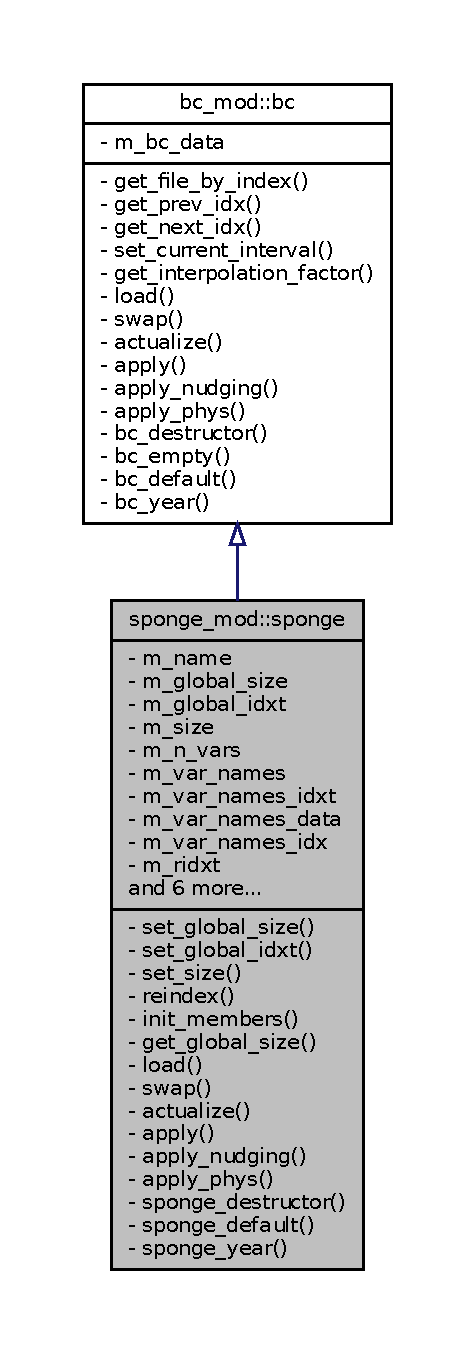
\includegraphics[height=550pt]{structsponge__mod_1_1sponge__inherit__graph}
\end{center}
\end{figure}
\subsubsection*{Private Member Functions}
\begin{DoxyCompactItemize}
\item 
procedure \mbox{\hyperlink{structsponge__mod_1_1sponge_afa5fb267b1d59f3b18ee94035a4816e3}{set\+\_\+global\+\_\+size}}
\item 
procedure \mbox{\hyperlink{structsponge__mod_1_1sponge_a2e1d0efffaf26aef18699231850069c5}{set\+\_\+global\+\_\+idxt}}
\item 
procedure \mbox{\hyperlink{structsponge__mod_1_1sponge_a2da2baff3ceb54811626114035885989}{set\+\_\+size}}
\item 
procedure \mbox{\hyperlink{structsponge__mod_1_1sponge_a8ea78d5f48aff24e7fd7ac5478e2bbc4}{reindex}}
\item 
procedure \mbox{\hyperlink{structsponge__mod_1_1sponge_a2b045a0f566da7df427aa0b776f92aa2}{init\+\_\+members}}
\item 
procedure \mbox{\hyperlink{structsponge__mod_1_1sponge_a6e25af9d9685756eca68b255dcbefde4}{get\+\_\+global\+\_\+size}}
\item 
procedure \mbox{\hyperlink{structsponge__mod_1_1sponge_a0383aabeecf15b7c47bc43c9b4746c60}{load}}
\item 
procedure \mbox{\hyperlink{structsponge__mod_1_1sponge_abe0102a0a72e189b8871724a21680c43}{swap}}
\item 
procedure \mbox{\hyperlink{structsponge__mod_1_1sponge_a7d01836ef5f2e2ea4ee11a6c6231baed}{actualize}}
\item 
procedure \mbox{\hyperlink{structsponge__mod_1_1sponge_aca76f3cc282e1918ec76c8d6c34d4315}{apply}}
\item 
procedure \mbox{\hyperlink{structsponge__mod_1_1sponge_a8617d126acfe553a2d478258adaf029f}{apply\+\_\+nudging}}
\item 
procedure \mbox{\hyperlink{structsponge__mod_1_1sponge_ab3f6fd55b37a4a4ba7fe9d0ac9f7b9ac}{apply\+\_\+phys}}
\item 
procedure \mbox{\hyperlink{structsponge__mod_1_1sponge_a592cfa3fa593c79ee6e25dfbe0b22025}{sponge\+\_\+destructor}}
\item 
type(\mbox{\hyperlink{structsponge__mod_1_1sponge}{sponge}}) function \mbox{\hyperlink{structsponge__mod_1_1sponge_afb942e8b46de1f0ea4de815db78a9c62}{sponge\+\_\+default}} (files\+\_\+namelist, bc\+\_\+name, n\+\_\+vars, vars, var\+\_\+names\+\_\+idx, alpha, reduction\+\_\+value\+\_\+t, length)
\item 
type(\mbox{\hyperlink{structsponge__mod_1_1sponge}{sponge}}) function \mbox{\hyperlink{structsponge__mod_1_1sponge_a9f7844c5d77b32ce566d362f29d4b816}{sponge\+\_\+year}} (files\+\_\+namelist, bc\+\_\+name, n\+\_\+vars, vars, var\+\_\+names\+\_\+idx, alpha, reduction\+\_\+value\+\_\+t, length, start\+\_\+time\+\_\+string, end\+\_\+time\+\_\+string)
\end{DoxyCompactItemize}
\subsubsection*{Private Attributes}
\begin{DoxyCompactItemize}
\item 
character(len=3) \mbox{\hyperlink{structsponge__mod_1_1sponge_a2772acd01b2159e7538ae075bb79d002}{m\+\_\+name}}
\item 
integer(4) \mbox{\hyperlink{structsponge__mod_1_1sponge_a013fe29d72c3bb46d15e484c75319dab}{m\+\_\+global\+\_\+size}}
\item 
integer(4), dimension(\+:), allocatable \mbox{\hyperlink{structsponge__mod_1_1sponge_ae8abf3ac8cf4f449ad890c0f892c5cfc}{m\+\_\+global\+\_\+idxt}}
\item 
integer(4) \mbox{\hyperlink{structsponge__mod_1_1sponge_aea00d9b1a185ddbedbed0fb7ee735950}{m\+\_\+size}}
\item 
integer \mbox{\hyperlink{structsponge__mod_1_1sponge_a3593de7bf7fc4415e27ef61d00a741f3}{m\+\_\+n\+\_\+vars}}
\item 
character(len=3), dimension(\+:), allocatable \mbox{\hyperlink{structsponge__mod_1_1sponge_ab1680a427e7b0bc1ffa592cd4981bef3}{m\+\_\+var\+\_\+names}}
\item 
character(len=12), dimension(\+:), allocatable \mbox{\hyperlink{structsponge__mod_1_1sponge_a6e80ea1bddd446d18272998fd99bfb0e}{m\+\_\+var\+\_\+names\+\_\+idxt}}
\item 
character(len=7), dimension(\+:), allocatable \mbox{\hyperlink{structsponge__mod_1_1sponge_a92d436c4342008e48be50f8a24763126}{m\+\_\+var\+\_\+names\+\_\+data}}
\item 
integer(4), dimension(\+:), allocatable \mbox{\hyperlink{structsponge__mod_1_1sponge_ae9500658821f8133f368d3498ae29bff}{m\+\_\+var\+\_\+names\+\_\+idx}}
\item 
integer(4), dimension(\+:, \+:), allocatable \mbox{\hyperlink{structsponge__mod_1_1sponge_a8eb04cbc3c298283d7d41b96afe68303}{m\+\_\+ridxt}}
\item 
double precision, dimension(\+:), allocatable \mbox{\hyperlink{structsponge__mod_1_1sponge_a1bb1f743a4745eb7b76d647ac7299a10}{m\+\_\+aux}}
\item 
double precision, dimension(\+:, \+:, \+:), allocatable \mbox{\hyperlink{structsponge__mod_1_1sponge_a2edf92416fc98db4d8105f6c7a7c3aaa}{m\+\_\+values\+\_\+dtatrc}}
\item 
double precision, dimension(\+:, \+:), allocatable \mbox{\hyperlink{structsponge__mod_1_1sponge_ae5b49e184aac449a582c2b35149bfafa}{m\+\_\+values}}
\item 
double precision \mbox{\hyperlink{structsponge__mod_1_1sponge_aeb3b50dcf03f861abad13b7b12697ff5}{m\+\_\+alpha}}
\item 
double precision \mbox{\hyperlink{structsponge__mod_1_1sponge_a7d79ba225284f05c08fa8126ec467c72}{m\+\_\+reduction\+\_\+value\+\_\+t}}
\item 
double precision \mbox{\hyperlink{structsponge__mod_1_1sponge_ae224137cda346dac603ed0412ccd8c2d}{m\+\_\+length}}
\end{DoxyCompactItemize}


\subsubsection{Member Function/\+Subroutine Documentation}
\mbox{\Hypertarget{structsponge__mod_1_1sponge_a7d01836ef5f2e2ea4ee11a6c6231baed}\label{structsponge__mod_1_1sponge_a7d01836ef5f2e2ea4ee11a6c6231baed}} 
\index{sponge\+\_\+mod\+::sponge@{sponge\+\_\+mod\+::sponge}!actualize@{actualize}}
\index{actualize@{actualize}!sponge\+\_\+mod\+::sponge@{sponge\+\_\+mod\+::sponge}}
\paragraph{\texorpdfstring{actualize()}{actualize()}}
{\footnotesize\ttfamily procedure sponge\+\_\+mod\+::sponge\+::actualize (\begin{DoxyParamCaption}{ }\end{DoxyParamCaption})\hspace{0.3cm}{\ttfamily [private]}}



Implements \mbox{\hyperlink{structbc__mod_1_1bc_a15503494f181d4090774d948cecdce48}{bc\+\_\+mod\+::bc}}.

\mbox{\Hypertarget{structsponge__mod_1_1sponge_aca76f3cc282e1918ec76c8d6c34d4315}\label{structsponge__mod_1_1sponge_aca76f3cc282e1918ec76c8d6c34d4315}} 
\index{sponge\+\_\+mod\+::sponge@{sponge\+\_\+mod\+::sponge}!apply@{apply}}
\index{apply@{apply}!sponge\+\_\+mod\+::sponge@{sponge\+\_\+mod\+::sponge}}
\paragraph{\texorpdfstring{apply()}{apply()}}
{\footnotesize\ttfamily procedure sponge\+\_\+mod\+::sponge\+::apply (\begin{DoxyParamCaption}{ }\end{DoxyParamCaption})\hspace{0.3cm}{\ttfamily [private]}}



Implements \mbox{\hyperlink{structbc__mod_1_1bc_a628eafc79842d1d1d62e043aedf49aa0}{bc\+\_\+mod\+::bc}}.

\mbox{\Hypertarget{structsponge__mod_1_1sponge_a8617d126acfe553a2d478258adaf029f}\label{structsponge__mod_1_1sponge_a8617d126acfe553a2d478258adaf029f}} 
\index{sponge\+\_\+mod\+::sponge@{sponge\+\_\+mod\+::sponge}!apply\+\_\+nudging@{apply\+\_\+nudging}}
\index{apply\+\_\+nudging@{apply\+\_\+nudging}!sponge\+\_\+mod\+::sponge@{sponge\+\_\+mod\+::sponge}}
\paragraph{\texorpdfstring{apply\+\_\+nudging()}{apply\_nudging()}}
{\footnotesize\ttfamily procedure sponge\+\_\+mod\+::sponge\+::apply\+\_\+nudging (\begin{DoxyParamCaption}{ }\end{DoxyParamCaption})\hspace{0.3cm}{\ttfamily [private]}}



Implements \mbox{\hyperlink{structbc__mod_1_1bc_a42dc448ba9e50fbb6b1acf03b0d121f3}{bc\+\_\+mod\+::bc}}.

\mbox{\Hypertarget{structsponge__mod_1_1sponge_ab3f6fd55b37a4a4ba7fe9d0ac9f7b9ac}\label{structsponge__mod_1_1sponge_ab3f6fd55b37a4a4ba7fe9d0ac9f7b9ac}} 
\index{sponge\+\_\+mod\+::sponge@{sponge\+\_\+mod\+::sponge}!apply\+\_\+phys@{apply\+\_\+phys}}
\index{apply\+\_\+phys@{apply\+\_\+phys}!sponge\+\_\+mod\+::sponge@{sponge\+\_\+mod\+::sponge}}
\paragraph{\texorpdfstring{apply\+\_\+phys()}{apply\_phys()}}
{\footnotesize\ttfamily procedure sponge\+\_\+mod\+::sponge\+::apply\+\_\+phys (\begin{DoxyParamCaption}{ }\end{DoxyParamCaption})\hspace{0.3cm}{\ttfamily [private]}}



Implements \mbox{\hyperlink{structbc__mod_1_1bc_ad0d03ece320569369a296ff3d4cf10d2}{bc\+\_\+mod\+::bc}}.

\mbox{\Hypertarget{structsponge__mod_1_1sponge_a6e25af9d9685756eca68b255dcbefde4}\label{structsponge__mod_1_1sponge_a6e25af9d9685756eca68b255dcbefde4}} 
\index{sponge\+\_\+mod\+::sponge@{sponge\+\_\+mod\+::sponge}!get\+\_\+global\+\_\+size@{get\+\_\+global\+\_\+size}}
\index{get\+\_\+global\+\_\+size@{get\+\_\+global\+\_\+size}!sponge\+\_\+mod\+::sponge@{sponge\+\_\+mod\+::sponge}}
\paragraph{\texorpdfstring{get\+\_\+global\+\_\+size()}{get\_global\_size()}}
{\footnotesize\ttfamily procedure sponge\+\_\+mod\+::sponge\+::get\+\_\+global\+\_\+size (\begin{DoxyParamCaption}{ }\end{DoxyParamCaption})\hspace{0.3cm}{\ttfamily [private]}}

\mbox{\Hypertarget{structsponge__mod_1_1sponge_a2b045a0f566da7df427aa0b776f92aa2}\label{structsponge__mod_1_1sponge_a2b045a0f566da7df427aa0b776f92aa2}} 
\index{sponge\+\_\+mod\+::sponge@{sponge\+\_\+mod\+::sponge}!init\+\_\+members@{init\+\_\+members}}
\index{init\+\_\+members@{init\+\_\+members}!sponge\+\_\+mod\+::sponge@{sponge\+\_\+mod\+::sponge}}
\paragraph{\texorpdfstring{init\+\_\+members()}{init\_members()}}
{\footnotesize\ttfamily procedure sponge\+\_\+mod\+::sponge\+::init\+\_\+members (\begin{DoxyParamCaption}{ }\end{DoxyParamCaption})\hspace{0.3cm}{\ttfamily [private]}}

\mbox{\Hypertarget{structsponge__mod_1_1sponge_a0383aabeecf15b7c47bc43c9b4746c60}\label{structsponge__mod_1_1sponge_a0383aabeecf15b7c47bc43c9b4746c60}} 
\index{sponge\+\_\+mod\+::sponge@{sponge\+\_\+mod\+::sponge}!load@{load}}
\index{load@{load}!sponge\+\_\+mod\+::sponge@{sponge\+\_\+mod\+::sponge}}
\paragraph{\texorpdfstring{load()}{load()}}
{\footnotesize\ttfamily procedure sponge\+\_\+mod\+::sponge\+::load (\begin{DoxyParamCaption}{ }\end{DoxyParamCaption})\hspace{0.3cm}{\ttfamily [private]}}



Implements \mbox{\hyperlink{structbc__mod_1_1bc_a1c4ee986270f18f4400c4554c06c5f7b}{bc\+\_\+mod\+::bc}}.

\mbox{\Hypertarget{structsponge__mod_1_1sponge_a8ea78d5f48aff24e7fd7ac5478e2bbc4}\label{structsponge__mod_1_1sponge_a8ea78d5f48aff24e7fd7ac5478e2bbc4}} 
\index{sponge\+\_\+mod\+::sponge@{sponge\+\_\+mod\+::sponge}!reindex@{reindex}}
\index{reindex@{reindex}!sponge\+\_\+mod\+::sponge@{sponge\+\_\+mod\+::sponge}}
\paragraph{\texorpdfstring{reindex()}{reindex()}}
{\footnotesize\ttfamily procedure sponge\+\_\+mod\+::sponge\+::reindex (\begin{DoxyParamCaption}{ }\end{DoxyParamCaption})\hspace{0.3cm}{\ttfamily [private]}}

\mbox{\Hypertarget{structsponge__mod_1_1sponge_a2e1d0efffaf26aef18699231850069c5}\label{structsponge__mod_1_1sponge_a2e1d0efffaf26aef18699231850069c5}} 
\index{sponge\+\_\+mod\+::sponge@{sponge\+\_\+mod\+::sponge}!set\+\_\+global\+\_\+idxt@{set\+\_\+global\+\_\+idxt}}
\index{set\+\_\+global\+\_\+idxt@{set\+\_\+global\+\_\+idxt}!sponge\+\_\+mod\+::sponge@{sponge\+\_\+mod\+::sponge}}
\paragraph{\texorpdfstring{set\+\_\+global\+\_\+idxt()}{set\_global\_idxt()}}
{\footnotesize\ttfamily procedure sponge\+\_\+mod\+::sponge\+::set\+\_\+global\+\_\+idxt (\begin{DoxyParamCaption}{ }\end{DoxyParamCaption})\hspace{0.3cm}{\ttfamily [private]}}

\mbox{\Hypertarget{structsponge__mod_1_1sponge_afa5fb267b1d59f3b18ee94035a4816e3}\label{structsponge__mod_1_1sponge_afa5fb267b1d59f3b18ee94035a4816e3}} 
\index{sponge\+\_\+mod\+::sponge@{sponge\+\_\+mod\+::sponge}!set\+\_\+global\+\_\+size@{set\+\_\+global\+\_\+size}}
\index{set\+\_\+global\+\_\+size@{set\+\_\+global\+\_\+size}!sponge\+\_\+mod\+::sponge@{sponge\+\_\+mod\+::sponge}}
\paragraph{\texorpdfstring{set\+\_\+global\+\_\+size()}{set\_global\_size()}}
{\footnotesize\ttfamily procedure sponge\+\_\+mod\+::sponge\+::set\+\_\+global\+\_\+size (\begin{DoxyParamCaption}{ }\end{DoxyParamCaption})\hspace{0.3cm}{\ttfamily [private]}}

\mbox{\Hypertarget{structsponge__mod_1_1sponge_a2da2baff3ceb54811626114035885989}\label{structsponge__mod_1_1sponge_a2da2baff3ceb54811626114035885989}} 
\index{sponge\+\_\+mod\+::sponge@{sponge\+\_\+mod\+::sponge}!set\+\_\+size@{set\+\_\+size}}
\index{set\+\_\+size@{set\+\_\+size}!sponge\+\_\+mod\+::sponge@{sponge\+\_\+mod\+::sponge}}
\paragraph{\texorpdfstring{set\+\_\+size()}{set\_size()}}
{\footnotesize\ttfamily procedure sponge\+\_\+mod\+::sponge\+::set\+\_\+size (\begin{DoxyParamCaption}{ }\end{DoxyParamCaption})\hspace{0.3cm}{\ttfamily [private]}}

\mbox{\Hypertarget{structsponge__mod_1_1sponge_afb942e8b46de1f0ea4de815db78a9c62}\label{structsponge__mod_1_1sponge_afb942e8b46de1f0ea4de815db78a9c62}} 
\index{sponge\+\_\+mod\+::sponge@{sponge\+\_\+mod\+::sponge}!sponge\+\_\+default@{sponge\+\_\+default}}
\index{sponge\+\_\+default@{sponge\+\_\+default}!sponge\+\_\+mod\+::sponge@{sponge\+\_\+mod\+::sponge}}
\paragraph{\texorpdfstring{sponge\+\_\+default()}{sponge\_default()}}
{\footnotesize\ttfamily type(\mbox{\hyperlink{structsponge__mod_1_1sponge}{sponge}}) function sponge\+\_\+mod\+::sponge\+::sponge\+\_\+default (\begin{DoxyParamCaption}\item[{character(len=22), intent(in)}]{files\+\_\+namelist,  }\item[{character(len=3)}]{bc\+\_\+name,  }\item[{integer, intent(in)}]{n\+\_\+vars,  }\item[{character(len=27), intent(in)}]{vars,  }\item[{integer(4), dimension(n\+\_\+vars), intent(in)}]{var\+\_\+names\+\_\+idx,  }\item[{double precision, intent(in)}]{alpha,  }\item[{double precision, intent(in)}]{reduction\+\_\+value\+\_\+t,  }\item[{double precision, intent(in)}]{length }\end{DoxyParamCaption})\hspace{0.3cm}{\ttfamily [private]}}

\mbox{\Hypertarget{structsponge__mod_1_1sponge_a592cfa3fa593c79ee6e25dfbe0b22025}\label{structsponge__mod_1_1sponge_a592cfa3fa593c79ee6e25dfbe0b22025}} 
\index{sponge\+\_\+mod\+::sponge@{sponge\+\_\+mod\+::sponge}!sponge\+\_\+destructor@{sponge\+\_\+destructor}}
\index{sponge\+\_\+destructor@{sponge\+\_\+destructor}!sponge\+\_\+mod\+::sponge@{sponge\+\_\+mod\+::sponge}}
\paragraph{\texorpdfstring{sponge\+\_\+destructor()}{sponge\_destructor()}}
{\footnotesize\ttfamily procedure sponge\+\_\+mod\+::sponge\+::sponge\+\_\+destructor (\begin{DoxyParamCaption}{ }\end{DoxyParamCaption})\hspace{0.3cm}{\ttfamily [private]}}

\mbox{\Hypertarget{structsponge__mod_1_1sponge_a9f7844c5d77b32ce566d362f29d4b816}\label{structsponge__mod_1_1sponge_a9f7844c5d77b32ce566d362f29d4b816}} 
\index{sponge\+\_\+mod\+::sponge@{sponge\+\_\+mod\+::sponge}!sponge\+\_\+year@{sponge\+\_\+year}}
\index{sponge\+\_\+year@{sponge\+\_\+year}!sponge\+\_\+mod\+::sponge@{sponge\+\_\+mod\+::sponge}}
\paragraph{\texorpdfstring{sponge\+\_\+year()}{sponge\_year()}}
{\footnotesize\ttfamily type(\mbox{\hyperlink{structsponge__mod_1_1sponge}{sponge}}) function sponge\+\_\+mod\+::sponge\+::sponge\+\_\+year (\begin{DoxyParamCaption}\item[{character(len=27), intent(in)}]{files\+\_\+namelist,  }\item[{character(len=3)}]{bc\+\_\+name,  }\item[{integer, intent(in)}]{n\+\_\+vars,  }\item[{character(len=27), intent(in)}]{vars,  }\item[{integer(4), dimension(n\+\_\+vars), intent(in)}]{var\+\_\+names\+\_\+idx,  }\item[{double precision, intent(in)}]{alpha,  }\item[{double precision, intent(in)}]{reduction\+\_\+value\+\_\+t,  }\item[{double precision, intent(in)}]{length,  }\item[{character(len=17), intent(in)}]{start\+\_\+time\+\_\+string,  }\item[{character(len=17), intent(in)}]{end\+\_\+time\+\_\+string }\end{DoxyParamCaption})\hspace{0.3cm}{\ttfamily [private]}}

\mbox{\Hypertarget{structsponge__mod_1_1sponge_abe0102a0a72e189b8871724a21680c43}\label{structsponge__mod_1_1sponge_abe0102a0a72e189b8871724a21680c43}} 
\index{sponge\+\_\+mod\+::sponge@{sponge\+\_\+mod\+::sponge}!swap@{swap}}
\index{swap@{swap}!sponge\+\_\+mod\+::sponge@{sponge\+\_\+mod\+::sponge}}
\paragraph{\texorpdfstring{swap()}{swap()}}
{\footnotesize\ttfamily procedure sponge\+\_\+mod\+::sponge\+::swap (\begin{DoxyParamCaption}{ }\end{DoxyParamCaption})\hspace{0.3cm}{\ttfamily [private]}}



Implements \mbox{\hyperlink{structbc__mod_1_1bc_a925ae5960dbfc854eab908c52c13f719}{bc\+\_\+mod\+::bc}}.



\subsubsection{Member Data Documentation}
\mbox{\Hypertarget{structsponge__mod_1_1sponge_aeb3b50dcf03f861abad13b7b12697ff5}\label{structsponge__mod_1_1sponge_aeb3b50dcf03f861abad13b7b12697ff5}} 
\index{sponge\+\_\+mod\+::sponge@{sponge\+\_\+mod\+::sponge}!m\+\_\+alpha@{m\+\_\+alpha}}
\index{m\+\_\+alpha@{m\+\_\+alpha}!sponge\+\_\+mod\+::sponge@{sponge\+\_\+mod\+::sponge}}
\paragraph{\texorpdfstring{m\+\_\+alpha}{m\_alpha}}
{\footnotesize\ttfamily double precision sponge\+\_\+mod\+::sponge\+::m\+\_\+alpha\hspace{0.3cm}{\ttfamily [private]}}

\mbox{\Hypertarget{structsponge__mod_1_1sponge_a1bb1f743a4745eb7b76d647ac7299a10}\label{structsponge__mod_1_1sponge_a1bb1f743a4745eb7b76d647ac7299a10}} 
\index{sponge\+\_\+mod\+::sponge@{sponge\+\_\+mod\+::sponge}!m\+\_\+aux@{m\+\_\+aux}}
\index{m\+\_\+aux@{m\+\_\+aux}!sponge\+\_\+mod\+::sponge@{sponge\+\_\+mod\+::sponge}}
\paragraph{\texorpdfstring{m\+\_\+aux}{m\_aux}}
{\footnotesize\ttfamily double precision, dimension(\+:), allocatable sponge\+\_\+mod\+::sponge\+::m\+\_\+aux\hspace{0.3cm}{\ttfamily [private]}}

\mbox{\Hypertarget{structsponge__mod_1_1sponge_ae8abf3ac8cf4f449ad890c0f892c5cfc}\label{structsponge__mod_1_1sponge_ae8abf3ac8cf4f449ad890c0f892c5cfc}} 
\index{sponge\+\_\+mod\+::sponge@{sponge\+\_\+mod\+::sponge}!m\+\_\+global\+\_\+idxt@{m\+\_\+global\+\_\+idxt}}
\index{m\+\_\+global\+\_\+idxt@{m\+\_\+global\+\_\+idxt}!sponge\+\_\+mod\+::sponge@{sponge\+\_\+mod\+::sponge}}
\paragraph{\texorpdfstring{m\+\_\+global\+\_\+idxt}{m\_global\_idxt}}
{\footnotesize\ttfamily integer(4), dimension(\+:), allocatable sponge\+\_\+mod\+::sponge\+::m\+\_\+global\+\_\+idxt\hspace{0.3cm}{\ttfamily [private]}}

\mbox{\Hypertarget{structsponge__mod_1_1sponge_a013fe29d72c3bb46d15e484c75319dab}\label{structsponge__mod_1_1sponge_a013fe29d72c3bb46d15e484c75319dab}} 
\index{sponge\+\_\+mod\+::sponge@{sponge\+\_\+mod\+::sponge}!m\+\_\+global\+\_\+size@{m\+\_\+global\+\_\+size}}
\index{m\+\_\+global\+\_\+size@{m\+\_\+global\+\_\+size}!sponge\+\_\+mod\+::sponge@{sponge\+\_\+mod\+::sponge}}
\paragraph{\texorpdfstring{m\+\_\+global\+\_\+size}{m\_global\_size}}
{\footnotesize\ttfamily integer(4) sponge\+\_\+mod\+::sponge\+::m\+\_\+global\+\_\+size\hspace{0.3cm}{\ttfamily [private]}}

\mbox{\Hypertarget{structsponge__mod_1_1sponge_ae224137cda346dac603ed0412ccd8c2d}\label{structsponge__mod_1_1sponge_ae224137cda346dac603ed0412ccd8c2d}} 
\index{sponge\+\_\+mod\+::sponge@{sponge\+\_\+mod\+::sponge}!m\+\_\+length@{m\+\_\+length}}
\index{m\+\_\+length@{m\+\_\+length}!sponge\+\_\+mod\+::sponge@{sponge\+\_\+mod\+::sponge}}
\paragraph{\texorpdfstring{m\+\_\+length}{m\_length}}
{\footnotesize\ttfamily double precision sponge\+\_\+mod\+::sponge\+::m\+\_\+length\hspace{0.3cm}{\ttfamily [private]}}

\mbox{\Hypertarget{structsponge__mod_1_1sponge_a3593de7bf7fc4415e27ef61d00a741f3}\label{structsponge__mod_1_1sponge_a3593de7bf7fc4415e27ef61d00a741f3}} 
\index{sponge\+\_\+mod\+::sponge@{sponge\+\_\+mod\+::sponge}!m\+\_\+n\+\_\+vars@{m\+\_\+n\+\_\+vars}}
\index{m\+\_\+n\+\_\+vars@{m\+\_\+n\+\_\+vars}!sponge\+\_\+mod\+::sponge@{sponge\+\_\+mod\+::sponge}}
\paragraph{\texorpdfstring{m\+\_\+n\+\_\+vars}{m\_n\_vars}}
{\footnotesize\ttfamily integer sponge\+\_\+mod\+::sponge\+::m\+\_\+n\+\_\+vars\hspace{0.3cm}{\ttfamily [private]}}

\mbox{\Hypertarget{structsponge__mod_1_1sponge_a2772acd01b2159e7538ae075bb79d002}\label{structsponge__mod_1_1sponge_a2772acd01b2159e7538ae075bb79d002}} 
\index{sponge\+\_\+mod\+::sponge@{sponge\+\_\+mod\+::sponge}!m\+\_\+name@{m\+\_\+name}}
\index{m\+\_\+name@{m\+\_\+name}!sponge\+\_\+mod\+::sponge@{sponge\+\_\+mod\+::sponge}}
\paragraph{\texorpdfstring{m\+\_\+name}{m\_name}}
{\footnotesize\ttfamily character(len=3) sponge\+\_\+mod\+::sponge\+::m\+\_\+name\hspace{0.3cm}{\ttfamily [private]}}

\mbox{\Hypertarget{structsponge__mod_1_1sponge_a7d79ba225284f05c08fa8126ec467c72}\label{structsponge__mod_1_1sponge_a7d79ba225284f05c08fa8126ec467c72}} 
\index{sponge\+\_\+mod\+::sponge@{sponge\+\_\+mod\+::sponge}!m\+\_\+reduction\+\_\+value\+\_\+t@{m\+\_\+reduction\+\_\+value\+\_\+t}}
\index{m\+\_\+reduction\+\_\+value\+\_\+t@{m\+\_\+reduction\+\_\+value\+\_\+t}!sponge\+\_\+mod\+::sponge@{sponge\+\_\+mod\+::sponge}}
\paragraph{\texorpdfstring{m\+\_\+reduction\+\_\+value\+\_\+t}{m\_reduction\_value\_t}}
{\footnotesize\ttfamily double precision sponge\+\_\+mod\+::sponge\+::m\+\_\+reduction\+\_\+value\+\_\+t\hspace{0.3cm}{\ttfamily [private]}}

\mbox{\Hypertarget{structsponge__mod_1_1sponge_a8eb04cbc3c298283d7d41b96afe68303}\label{structsponge__mod_1_1sponge_a8eb04cbc3c298283d7d41b96afe68303}} 
\index{sponge\+\_\+mod\+::sponge@{sponge\+\_\+mod\+::sponge}!m\+\_\+ridxt@{m\+\_\+ridxt}}
\index{m\+\_\+ridxt@{m\+\_\+ridxt}!sponge\+\_\+mod\+::sponge@{sponge\+\_\+mod\+::sponge}}
\paragraph{\texorpdfstring{m\+\_\+ridxt}{m\_ridxt}}
{\footnotesize\ttfamily integer(4), dimension(\+:, \+:), allocatable sponge\+\_\+mod\+::sponge\+::m\+\_\+ridxt\hspace{0.3cm}{\ttfamily [private]}}

\mbox{\Hypertarget{structsponge__mod_1_1sponge_aea00d9b1a185ddbedbed0fb7ee735950}\label{structsponge__mod_1_1sponge_aea00d9b1a185ddbedbed0fb7ee735950}} 
\index{sponge\+\_\+mod\+::sponge@{sponge\+\_\+mod\+::sponge}!m\+\_\+size@{m\+\_\+size}}
\index{m\+\_\+size@{m\+\_\+size}!sponge\+\_\+mod\+::sponge@{sponge\+\_\+mod\+::sponge}}
\paragraph{\texorpdfstring{m\+\_\+size}{m\_size}}
{\footnotesize\ttfamily integer(4) sponge\+\_\+mod\+::sponge\+::m\+\_\+size\hspace{0.3cm}{\ttfamily [private]}}

\mbox{\Hypertarget{structsponge__mod_1_1sponge_ae5b49e184aac449a582c2b35149bfafa}\label{structsponge__mod_1_1sponge_ae5b49e184aac449a582c2b35149bfafa}} 
\index{sponge\+\_\+mod\+::sponge@{sponge\+\_\+mod\+::sponge}!m\+\_\+values@{m\+\_\+values}}
\index{m\+\_\+values@{m\+\_\+values}!sponge\+\_\+mod\+::sponge@{sponge\+\_\+mod\+::sponge}}
\paragraph{\texorpdfstring{m\+\_\+values}{m\_values}}
{\footnotesize\ttfamily double precision, dimension(\+:, \+:), allocatable sponge\+\_\+mod\+::sponge\+::m\+\_\+values\hspace{0.3cm}{\ttfamily [private]}}

\mbox{\Hypertarget{structsponge__mod_1_1sponge_a2edf92416fc98db4d8105f6c7a7c3aaa}\label{structsponge__mod_1_1sponge_a2edf92416fc98db4d8105f6c7a7c3aaa}} 
\index{sponge\+\_\+mod\+::sponge@{sponge\+\_\+mod\+::sponge}!m\+\_\+values\+\_\+dtatrc@{m\+\_\+values\+\_\+dtatrc}}
\index{m\+\_\+values\+\_\+dtatrc@{m\+\_\+values\+\_\+dtatrc}!sponge\+\_\+mod\+::sponge@{sponge\+\_\+mod\+::sponge}}
\paragraph{\texorpdfstring{m\+\_\+values\+\_\+dtatrc}{m\_values\_dtatrc}}
{\footnotesize\ttfamily double precision, dimension(\+:, \+:, \+:), allocatable sponge\+\_\+mod\+::sponge\+::m\+\_\+values\+\_\+dtatrc\hspace{0.3cm}{\ttfamily [private]}}

\mbox{\Hypertarget{structsponge__mod_1_1sponge_ab1680a427e7b0bc1ffa592cd4981bef3}\label{structsponge__mod_1_1sponge_ab1680a427e7b0bc1ffa592cd4981bef3}} 
\index{sponge\+\_\+mod\+::sponge@{sponge\+\_\+mod\+::sponge}!m\+\_\+var\+\_\+names@{m\+\_\+var\+\_\+names}}
\index{m\+\_\+var\+\_\+names@{m\+\_\+var\+\_\+names}!sponge\+\_\+mod\+::sponge@{sponge\+\_\+mod\+::sponge}}
\paragraph{\texorpdfstring{m\+\_\+var\+\_\+names}{m\_var\_names}}
{\footnotesize\ttfamily character(len=3), dimension(\+:), allocatable sponge\+\_\+mod\+::sponge\+::m\+\_\+var\+\_\+names\hspace{0.3cm}{\ttfamily [private]}}

\mbox{\Hypertarget{structsponge__mod_1_1sponge_a92d436c4342008e48be50f8a24763126}\label{structsponge__mod_1_1sponge_a92d436c4342008e48be50f8a24763126}} 
\index{sponge\+\_\+mod\+::sponge@{sponge\+\_\+mod\+::sponge}!m\+\_\+var\+\_\+names\+\_\+data@{m\+\_\+var\+\_\+names\+\_\+data}}
\index{m\+\_\+var\+\_\+names\+\_\+data@{m\+\_\+var\+\_\+names\+\_\+data}!sponge\+\_\+mod\+::sponge@{sponge\+\_\+mod\+::sponge}}
\paragraph{\texorpdfstring{m\+\_\+var\+\_\+names\+\_\+data}{m\_var\_names\_data}}
{\footnotesize\ttfamily character(len=7), dimension(\+:), allocatable sponge\+\_\+mod\+::sponge\+::m\+\_\+var\+\_\+names\+\_\+data\hspace{0.3cm}{\ttfamily [private]}}

\mbox{\Hypertarget{structsponge__mod_1_1sponge_ae9500658821f8133f368d3498ae29bff}\label{structsponge__mod_1_1sponge_ae9500658821f8133f368d3498ae29bff}} 
\index{sponge\+\_\+mod\+::sponge@{sponge\+\_\+mod\+::sponge}!m\+\_\+var\+\_\+names\+\_\+idx@{m\+\_\+var\+\_\+names\+\_\+idx}}
\index{m\+\_\+var\+\_\+names\+\_\+idx@{m\+\_\+var\+\_\+names\+\_\+idx}!sponge\+\_\+mod\+::sponge@{sponge\+\_\+mod\+::sponge}}
\paragraph{\texorpdfstring{m\+\_\+var\+\_\+names\+\_\+idx}{m\_var\_names\_idx}}
{\footnotesize\ttfamily integer(4), dimension(\+:), allocatable sponge\+\_\+mod\+::sponge\+::m\+\_\+var\+\_\+names\+\_\+idx\hspace{0.3cm}{\ttfamily [private]}}

\mbox{\Hypertarget{structsponge__mod_1_1sponge_a6e80ea1bddd446d18272998fd99bfb0e}\label{structsponge__mod_1_1sponge_a6e80ea1bddd446d18272998fd99bfb0e}} 
\index{sponge\+\_\+mod\+::sponge@{sponge\+\_\+mod\+::sponge}!m\+\_\+var\+\_\+names\+\_\+idxt@{m\+\_\+var\+\_\+names\+\_\+idxt}}
\index{m\+\_\+var\+\_\+names\+\_\+idxt@{m\+\_\+var\+\_\+names\+\_\+idxt}!sponge\+\_\+mod\+::sponge@{sponge\+\_\+mod\+::sponge}}
\paragraph{\texorpdfstring{m\+\_\+var\+\_\+names\+\_\+idxt}{m\_var\_names\_idxt}}
{\footnotesize\ttfamily character(len=12), dimension(\+:), allocatable sponge\+\_\+mod\+::sponge\+::m\+\_\+var\+\_\+names\+\_\+idxt\hspace{0.3cm}{\ttfamily [private]}}


%--- End generated contents ---

% Index
\newpage
\phantomsection
\clearemptydoublepage
\addcontentsline{toc}{section}{Index}
\printindex

\end{document}
